% !TEX encoding = UTF-8 Unicode
% !BIB TS-program = biber

% This file is MIT-Thesis.tex, a LaTeX template for formatting an MIT thesis with the mitthesis class.
%
% Version: 1.17, 2024/11/02
%
% Author: John H. Lienhard, copyright 2024. Reuse under the MIT license: https://ctan.org/license/mit 

% Documentation is here: https://ctan.org/pkg/mitthesis

%% Don't modify the \DocumentMetadata command unless you know what it does. 
%% If this command throws an "undefined" error, your latex system is out of date: try commenting this command out.
\DocumentMetadata{
	lang		= en-US,
	pdfversion  = 1.7,
	pdfstandard = a-2b,
%	 pdfversion  = 2.0,
%    pdfstandard = a-4,
%	 debug		= {xmp-export}, % creates and xmpi file useful for checking metadata
}

%%%%%%%%%%%%%%%%%%%%%%%%%%%%%%%%%%%%%%%

\documentclass[twoside]{mitthesis}% fontset=newtx, fontset=libertine, fontset=libertinus, fontset=lmodern, fontset=newtx-sans-text, fontset=fira-newtxsf, fontset=heros-stix2, fontset=stix2, fontset=lmodern
%
% option [twoside]		gives facing-page behavior for printing; omitting twoside will eliminate even-numbered blank pages.
% option [lineno]	 	provides line numbers, as for editing
% option [mydesign] 	loads packages for color, title and list formats, margins, or captions: edit mydesign.tex to change defaults.
% option [fontset] is a keyvalue which can be:
%					 	for pdftex or unicode engines:  defaultfonts, libertine, libertinus, lmodern, lucida
%					 	for pdftex only: 				fira-newtxsf, newtx, newtx-sans-text
%						for unicode engines (luatex):	heros-stix2, stix2, termes, termes-stix2
%					 	if no key value is given, fonts default to CMR (pdftex) or LMR (unicode), i.e., "the LaTeX font".
%					 	You can edit the fontset files or you can write your own, myfonts.tex, and do [fontset=myfonts].
%						If you are using multiple languages, load the babel package in your fontset file, before the fonts.

%%%%%%%%% Packages used in sample chapters (not otherwise required) %%%%%%%
\usepackage{float}
\usepackage[font=small,labelfont=bf]{caption}
%% Package for code listing in Appendix A.
\usepackage{listings}%   documentation is here https://ctan.org/pkg/listings
\usepackage{amsfonts}
\usepackage{amsmath}
\usepackage{algorithm}
\usepackage{algpseudocode}
\usepackage{setspace}
\onehalfspacing
%% Set chemical formulas nicely
\usepackage[version=4]{mhchem}%   documentation at https://ctan.org/pkg/mhchem
\usepackage{xcolor} % Add this in the preamble if not already present

\newcommand{\rOne}[1]{\textcolor{red}{#1}}
\newcommand{\rTwo}[1]{\textcolor{blue}{#1}}

\usepackage[colorinlistoftodos]{todonotes}

%% Latin filler used in Chapter 1, with a test for package version date (https://ctan.org/pkg/lipsum)
\usepackage{lipsum}
\IfPackageAtLeastTF{lipsum}{2021/09/20}{\setlipsum{auto-lang=false}}{}

%% Table related packages  

\usepackage{booktabs}% publication quality tables (https://ctan.org/pkg/booktabs)
\usepackage{multirow}
\usepackage{array}% Additional options for column formats (https://ctan.org/pkg/array)

\usepackage{dcolumn}% For alignment of numbers on the decimal place (https://ctan.org/pkg/dcolumn) 
  \newcolumntype{d}[1]{D{.}{.}{#1}}% use with dcolumn package. Note: dcolumns are set in math mode.
  % syntax: d{x.y} where x is max number of digits before decimal and y is max number after.

% Package for multipage table in Appendix B.
\usepackage{longtable}% typeset multi-page tables (https://ctan.org/pkg/longtable)

%\usepackage{tabularx}% adjustable-width columns in tabular (https://ctan.org/pkg/tabularx)


%% Package for improved typography

\usepackage{microtype}% typographic fine-tuning, used in sample thesis committee page, but also acting globally on the text 


%%%%%%%%%  Graphics path (to figure files)  %%%%%%%%%%%%%%%%%%%%%%%%%%%%%%%%

%% Can set graphicspath to point to specific directories containing figures (the current directory is searched automatically)
%% For instance, to search a subdirectory of the current directory called "figures" and a parallel directory called "art", set:

% \graphicspath{ {figures/} {../art/} }% For details see: https://latexref.xyz/dev/latex2e.html#g_t_005cgraphicspath


%%%%%%%%%  Representative set-up for biblatex  %%%%%%%%%%%%%%%%%%%%%%%%%%%%%

%% Numerical citations of references
\usepackage[style=ext-numeric-comp,giveninits=true,maxbibnames=10,sorting=none]{biblatex}
 
%% IEEE style citations and references
% \usepackage[style=ieee,maxbibnames=10,sorting=none]{biblatex}% style=ext-numeric-comp,articlein=false,giveninits=true
%	 \DefineBibliographyStrings{english}{url= \textsc{url} ,  }% replaces the IEEE default "[Online]. Available" by "URL"

%% author-year style citations and references 
%% use \parencite, not \cite, when you want "(Author, year)"
%% The sample files are not set up to include parentheses.
% \usepackage[style=authoryear, maxbibnames=10]{biblatex} 


\addbibresource{literature.bib}%% <== change to YOUR bib file <= CHANGE

%% to avoid split urls and stretched white space, you can set the bibliography ragged-right:
%\appto{\bibsetup}{\raggedright}

%% biblatex is very powerful, and you can customize most aspects the reference list and citations to suit your needs.
%%   documentation is here: https://ctan.org/pkg/biblatex
%%   cheat sheet is here:   https://tug.ctan.org/info/biblatex-cheatsheet/biblatex-cheatsheet.pdf 

%% To ensure citations are set, run Latex --> biblatex/biber --> Latex again

%%%%%%%%%%  Option to use natbib   %%%%%%%%%%%%%%%%%%%%%%%%%%%%%%%%%%%%%%%%%

%\RequirePackage[numbers,sort&compress]{natbib}
 
%%% add bibliography to table of contents
%\apptocmd{\bibliography}{\addcontentsline{toc}{chapter}{\protect\textbf{\bibname}}}{}{}

%%% You can use this to rename the bibliography section
%\renewcommand{\bibname}{References}

%%% To adjust space between bibliography items 
%\setlength\bibsep{4pt plus 1pt minus 1pt}
%   change 4pt to something else; don't drop last two lengths (they are stretchable "glue")


%%%%%%%%%%  Option for "double spacing" %%%%%%%%%%%%%%%%%%%%%%%%%%%%%%%%%%%%

%% Back in the typewriter era, double spaced lines were convenient for editing with a pencil. 
%% In typography, the separation between lines is called "leading", and it is usually set in 
%% proportion to the font size (i.e., when the font is loaded).  If you really feel the need 
%% to change the line separation, the most attractive results will be obtained by changing the
%% leading in proportion to the the current font size, rather than just doubling the space.

%% The setspace package provides a tool for changing line separation. Use these two commands here:
%
% \usepackage{setspace}%  documentation at https://ctan.org/pkg/setspace
% \setstretch{1.1}% you can choose some other value for the stretch of space between lines
%
%% Use one or more of the these commands *AFTER* the frontmatter
%
% \onehalfspacing
% \doublespacing
% \singlespacing  % will turn these effects off (you can use these anywhere in the document)

%% The best result is usually to stay with leading selected by the typographer who set up the font.


%%%%%%%%%%%  Metadata  %%%%%%%%%%%%%%%%%%%%%%%%%%%%%%%%%%%%%%%%%%%%%%%%%%%%%%%

% Most of the document metadata is created automatically. 
% The following items should be adjusted to match your work. <================= !!!!!!!!!!

\hypersetup{%
	pdfsubject={Template for writing MIT theses with the mitthesis class},
	% Change this to briefly state topic of your thesis 
% 
	pdfkeywords={Göttingen, Neuroinformatics},
	% Add keywords that will help search engines and libraries to find your work.
	% Includes the name[s] of the author[s] 
	% (If you used \DocumentMetadata at line 14, you can just put "\CopyrightAuthor," for the names.)
%
	pdfurl={},
	% If you have a url for the thesis, put it here. Otherwise delete this.
	% (MIT Libraries will put your thesis in DSPACE with a persistent url after you submit it.)
%	
	pdfcontactemail={},
	% You can put a [permanent] email address into the metadata, if you like.
	% Otherwise delete this.
%
	pdfauthortitle={},
	% If you have a title, you can include it here.
}

%%%%%%%%%%%%  Math operators %%%%%%%%%%%%%%%%%%%%%%%%%%%%%%%%%%%%%%%%%%%%%%%%%%%%

% These commands declare two math operators, \erf{..} and \erfc{..} using mathtools
% note: * form produces automatic delimiter scaling; optional argument sets size manually, e.g. [\bigg]
% See Table 1.1 in Chapter 1

\DeclareMathOperator{\Erf}{erf}
\DeclareMathOperator{\Erfc}{erfc}
\DeclarePairedDelimiterXPP\erf[1]{\Erf\mkern1mu} (){}{#1}% increase to 2mu with stix2 font
\DeclarePairedDelimiterXPP\erfc[1]{\Erfc\mkern1mu} (){}{#1}


%%%%%%%%%%%%%%  End preamble %%%%%%%%%%%%%%%%%%%%%%%%%%%%%%%%%%%%%%%%%%%%%%%%%%%%%%%%%%%%%%%%%%%%%
%%%%%%%%%%%%%%%%%%%%%%%%%%%%%%%%%%%%%%%%%%%%%%%%%%%%%%%%%%%%%%%%%%%%%%%%%%%%%%%%%%%%%%%%%%%%%%%%%%

\begin{document}
%%% edit the following commands to match your thesis %%%%%%%%%%

\title{Influence of data diversity in brain decoding: An empirical study of image reconstruction from fMRI data}

% \Author{Author full name}{Author department}[Author's first PREVIOUS degree][Author's second PREVIOUS degree][...
% Note that third, fourth, fifth, and sixth arguments are optional [] and may be omitted

% note on names: most of the following names are made up; Silas Holman was a physics professor at MIT in the 19th century.

\Author{Matthias K. Mildenberger}{Department of Computer Science}
% \Author{Luisa Hernández}{Department of Research}[B.S. Mechanical Engineering, UCLA, 2018][M.S. Stellar Interiors, Vulcan Science Academy, 2020]
% \Author{Thurston Howell III}{Department of Economics}[MBA, Ferengi School of Management, 2022]

% Use once for each degree fulfilled by thesis
% For two degrees from one department, leave the department argument blank for the second degree {}.
\Degree{Master of Science in Applied Computer Science}{Department of Computer Science}
%\Degree{Master of Science in Physics}{}
%\Degree{Bachelor of Science in Mechanical Engineering}{Department of Mechanical Engineering}

% If there is more than one supervisor, use the \Supervisor command for each.
\Supervisor{Yoshihiro Nagano}{Assistant Professor of Neuroinformatics}
% \Supervisor{Edward C. Pickering}{Professor of Physics, and \\ \> Professor of Something Else}
% \Supervisor{Secunda Castor}{Professor of Research}
% \Supervisor{Quintus Castor}{Professor of Log Dams}

% Professor who formally accepts theses for your department (e.g., the Graduate Officer, Professor Sméagol,...)
% If more than one department, use more than once
\Acceptor{Tertius Castor}{Professor of Log Dams}{Graduate Officer, Department of Research} % \\ \> Third title}

% \Acceptor{Quarta Castor}{Professor of Lodge Building}{Graduate Officer, Department of Mechanical Engineering}
%%%  If you need to reduce vertical space, put the acceptor title in the second argument and leave the third blank, {}.
% \Acceptor{Primus Castor}{Professor and Undergraduate Officer, Department of Physics}{}

% Usage: \DegreeDate{Month}{year}
% Valid degree months are February, May, June, or September
\DegreeDate{May}{2025}

% Date that final thesis is submitted to department
\ThesisDate{May 01, 2025}


%%%%%%  Choose whether to have a CREATIVE COMMONS License  %%%%%%%%%%%%%%%%%%%%%%%%%%%%%%%%%%%%%%
%
% If you are using a cc license, uncomment the following line and insert details of your cc license here.
%
% \CClicense{CC BY-NC-ND 4.0}{https://creativecommons.org/licenses/by-nc-nd/4.0/}
%

%%%%%%%  Solutions for overflowing titlepage  %%%%%%%%%%%%%%%%%%%%%%%%%%%%%%%%%%%%%%%%%%%%%%%%%%%

% If your title page is overflowing (from too many names, degrees, etc.):
%
% (a) you can reduce the 12pt and 18pt skips between various blocks to 6pt with this command:
%
% \Tighten
%
% (b)  you can scale down the Signature block at the bottom with this command:
%
% \SignatureBlockSize{\small}  %or this one \SignatureBlockSize{\footnotesize}
%
% (c) you can put the acceptor name and title onto two lines, rather than three like this:
%
% \Acceptor{Tertius Castor}{Professor and Graduate Officer, Department of Research}{}
%
% (d) you can change the font size of the author name[s] with
%
%	\AuthorNameSize{\normalsize}
%
% (e) and you can omit any previous degrees from the title page, instead mentioning them in the biographical sketch

% Also, if you prefer to keep the text toward the top of the page with most white space at the bottom, you
% can use this command to squash all of the vertical glue (stretchy space) with this command:
%
% \Squash 
%
% This command is useful when the text has not already reach the bottom of the page, since the glue gets squashed automatically
% when the page is too full.

%%%%%%%%%%%%%%%%%%%%%%%%%%%%%%%%%%%%%%%%%%%%%%%%%%%%%%%%%%%%%%%%%%%%%%%%%%%%%%%%%%%%%%%%%%%%%%%%%

%%% Make titlepage
\maketitle

%%%%%%%%% Contents that you need to write follows! %%%%%%%%%%%%%%%%%%%%%%%%%%%%%%%%%%%%%%%%%%%%%% 

% \includeonly{acknowledgments,biography,chapter1,chapter2,...,appendixa,...} 
%   for usage of includeonly, see https://latexref.xyz/_005cinclude-_0026-_005cincludeonly.html

%%% Frontmatter (write this material in the mentioned files)  %%%%%%%%%%%%%%%%%%%%%%%%%%%%%%%%%%%

% This page is optional. Edit the file committee_members.tex 
% % Sample thesis committee page for mitthesis.cls
% Version 1.01, 2024/10/08
%
% This page is not required by the MIT Libraries, but some departments require it.
%
% Insert between title page and abstract page.
% Format this page in any way that you like.  
% Add supervisor titles, degrees, and departments as appropriate.

%%%%% FORMATTING COMMANDS %%%%%%%%%%%%%%%%%%

%% Format title
\NewDocumentCommand\CommitteePageTitle{m}{
	\vspace*{75pt}%36pt}
	\IfPackageLoadedTF{microtype}
		{\textls*{\Large\textbf{\MakeUppercase{#1}}}}
		{{\Large\textbf{\MakeUppercase{#1}}}}%
	\pdfbookmark[0]{#1}{Committee}%
	\vspace*{10pt}%
}
% \textls* produces additional letter separation (appropriate for capitalized display text),
% PROVIDED THAT \usepackage{microtype} has been loaded in the preamble. 
% The extra space added is 100/1000 em (adjustable, see package documentation).

%% Format committee member subheadings
\NewDocumentCommand\Role{m}{
	\vspace*{50pt}%25pt}
	\IfPackageLoadedTF{microtype}
		{\textls*{\large{\textsc{#1}}}}
		{{\large\textsc{#1}}}%
	\vspace*{12pt}%
}

%%%%%%%%%%%%%%%%%%%%%%%%%%%%%%%%%%%%%%%%%%%%%

\begin{flushright}

\CommitteePageTitle{Thesis committee}

\Role{  }

 \textbf{Marcus Gavius Apicius} \\
 {\itshape
 Professor of Cooking Arts \\
 Department of Food Science \\
 }

\Role{Thesis Readers}

 \textbf{Marie-Antoine Carême} \\
 {\itshape
   Professor of Haute Cuisine \\
   Department of Food Science \\[18pt]
 }

 \textbf{Julia Child}\\
 {\itshape
   Professor of French Cuisine \\
   Department of Food Science \\[18pt]
 }

 \textbf{Miles Gloriosus} \\
 {\itshape
   Professor of Personal Pronouns \\
   Department of Rhetoric \\
 }

\end{flushright}

\cleardoublepage


% The abstract environment creates all the required headings and footers. 
% You only need to the text of the abstract in the file abstract.tex
\begin{abstract}
	% From mitthesis package
% Version: 1.01, 2023/06/19
% Documentation: https://ctan.org/pkg/mitthesis
%
% The abstract environment creates all the required headers and footnote. 
% You only need to add the text of the abstract itself.
%
% Approximately 500 words or less; try not to use formulas or special characters
% If you don't want an initial indentation, do \noindent at the start of the abstract

\noindent{}Reconstructing images directly from human brain activity was once considered science fiction; today, brain decoding using functional magnetic resonance imaging (fMRI) is turning this concept into reality. However, current methods lack the ability to properly reconstruct concepts that are not present in the training data. Recent findings in the field have shown that increasing the dimensions and thus the diversity of the training data may lead to better generalisation to unknown concepts. In this paper, three experiments are conducted to investigate the influence of training data diversity on the generalisation of image reconstruction algorithms and the ability to reconstruct images that are dissimilar to the training data. In the first experiment, diversity-based subsampling of the training data was performed to outperform a random subsampling baseline. In the second experiment, image captions were generated to emphasise the low-level (shape, colour) features of the training images, by using this approach the reconstruction of out-of-distribution (OOD) data could be improved. In the third experiment, perturbations were used to either increase or decrease the semantic value of the training data, the results of this experiment were inconclusive. In conclusion, the three experiments showed that the diversity of the dataset can play an important role in helping image reconstruction to generalise to unfamiliar concepts. Further research is needed to find the essential image dimensions needed in the data to create a universal image reconstruction method. It is also important to investigate how these dimensions correspond to the elicited brain activity.

% Yet, the accuracy of these reconstructions critically depends on the diversity of visual stimuli presented during training. This thesis explores how varying the richness and variety of training images influences the brain decoding process and ultimately determines the quality of reconstructed visual experiences.% use \input rather than \include because we're inside an environment
\end{abstract}

% %% acknowledgments.tex

% From mitthesis package
% Version: 1.02, 2024/06/19
% Documentation: https://ctan.org/pkg/mitthesis

\chapter*{Acknowledgments}
\pdfbookmark[0]{Acknowledgments}{acknowledgments}


I would like to express my deepest gratitude to my supervisor, Yoshihiro Nagano, for his excellent guidance throughout this work. His insigthful feedback, support in exploring and refining ideas and the thoughtful comments have been invaluable for me. Especially during times when the results did not align with my expectations he was able to motivate me and always find a new angle to view at the problems that eventually enabled me to make the next step forward. 

I would also like to thank Prof.\ Florentin Wörgötter for taking the role of second supervisor. Even though the topic was new to him, he was willing to support the work without hesitation. This gave me the unique opportunity to explore this interesting field. 

I also want to thank Linnéa Nöth for her support during the entire process. The engaging discussions, her help in structuring both my thoughts and the text, and encouragement during challenging moments kept me going. Thank you!

\section*{Software and Tools Used}

% Für diese Arbeit wurden diverse software und tools genutzt. Darunter die folgenden: Visual Studio Code als Editor für das Manuskript und den Programmcode, GitHub zur Versionierung des Manuskripts und des sourcecodes, Zotero zum Management der Literatur, LaTex zur Erstellung des fertigen Dokuments, ChatGPT zur Optimierung von Programmcode und der Diskussion von Formulierungen in der englischen Sprache, DeepL zur Übersetzung von der deutschen in die englische Sprache. Zusätzlich Google Scholar, Consensus.app und allen.ai paperfinder zur Literaturrecherche. 

Various software and tools were used in the course of this work, including the following: Visual Studio Code as the editor for both the manuscript and source code, GitHub for version control, Zotero for literature management, and LaTeX for compiling the final document. Additionally, ChatGPT was used to optimize programming code and to discuss English phrasings, DeepL supported translations from German into English. For literature research, Google Scholar, Consensus.app, and the Allen.ai PaperFinder were used. The exact libraries that have been used for the programming part of this thesis are listed in the according requirements of the conda environment in the GitHub repository of this work. 
% acknowledgments.tex (.tex extension is presumed by \include) 

% %% biography.tex
%% This section is optional

% From mitthesis package
% Version: 1.02, 2024/06/19
% Documentation: https://ctan.org/pkg/mitthesis

\chapter*{Biographical Sketch}
\pdfbookmark[0]{Biographical Sketch}{biosketch}


Silas Whitcomb Holman was born in Harvard, Massachusetts on January 20, 1856. He received his S.B. degree in Physics from MIT in 1876, and then joined the MIT Department of Physics as an Assistant. He became Instructor in Physics in 1880, Assistant Professor in 1882, Associate Professor in 1885, and Full Professor in 1893. Throughout this period, he struggled with increasingly severe rheumatoid arthritis. At length, he was defeated, becoming Professor Emeritus in 1897 and dying on April 1, 1900.

Holman's light burned brilliantly before his tragic and untimely death. He published extensively in thermal physics, and authored textbooks on precision measurement, fundamental mechanics, and other subjects. He established the original Heat Measurements Laboratory. Holman was a much admired teacher among both his students and his colleagues. The reports of his department and of the Institute itself refer to him frequently in the 1880's and 1890's, in tones that gradually shift from the greatest respect to the deepest sympathy.

Holman was a student of Professor Edward C. Pickering, then head of the Physics department. Holman himself became second in command of Physics, under Professor Charles R. Cross, some years later. Among Holman's students, several went on to distinguish themselves, including: the astronomer George E. Hale ('90) who organized the Yerkes and Mt. Wilson observatories and who designed the 200 inch telescope on Mt. Palomar; Charles G. Abbot ('94), also an astrophysicist and later Secretary of the Smithsonian Institution; and George K. Burgess ('96), later Director of the Bureau of Standards. % biography.tex (optional, see https://libraries.mit.edu/distinctive-collections/thesis-specs/#format)

%%% Table of contents and lists of stuff (delete unused lists, i.e., if no tables or figures) %%%%%

\tableofcontents
\listoffigures
% \listoftables

%%% Chapters of thesis  %%%%%%%%%%%%%%%%%%%%%%%%%%%%%%%%%%%%%%%%%%%%%%%%%%%%%%%%%%%%%%%%%%%%%%%%%%%

%% If you want to use "double spacing", you should start here...

 \chapter{Background}


- Datendiversität gibts auf unterschiedlichen Ebenen (das muss irgendwie mit drin sein für den Rest der Arbeit)
- Irgendwo auch schonmal irgendwie image naturalness droppen



- Versatile Diffusion \cite{xuVersatileDiffusionText2024} erklären

- Wir wollen einen Bildgenerator der universal ist, also Bilder mit ganz unterschiedlichen Charakteristika rekonstruieren kann. Zum Beispiel auch unabhängig von der Naturalness. Eine Möglichkeit naturalness zu messen ist in Multimedia Features for Click Prediction of New Ads in

- Modernere Bewertung zu was natural ist und was nicht in \cite{chenExploringNaturalnessAIGenerated2023}, folgt zwei verschiedenen Wegen wie der visual pathway

- Bei der Diversity kann man auch darauf eingehen, dass der visual pathway zwei verschiedene Wege folgt, in 20, 31, 66 aus \cite{chenExploringNaturalnessAIGenerated2023}

    - Genauso ist es sehr wichtig, dass eingeführt wird in das Konzept, dass es low-level und high-level Diversity geben kann, sodass die folgenden Kapitel (insbesondere dropout) darauf aufbauen können% .tex extension is presumed
 \chapter{Methodology}

\section{Data collection}


\rThree{This project uses an open fMRI dataset from previous studies by the Kamitani lab~\cite{guohuashenDeepImageReconstruction2020,horikawaGenericDecodingSeen2017}. Details of the data collection process are provided below.}

\subsection{Subjects}
The data were collected from 5 healthy volunteers aged between 23 and 33 years (4 males and 1 female). All subjects provided informed consent before the experiment, with the study protocol having been reviewed and approved by the Ethics Committee of the Graduate School of Informatics at Kyoto University (approval no.: KUIS{-}EAR{-}2017{-}002). The subjects had normal or corrected-to-normal vision. \rThree{The recorded data of three of the participants is pubclicly available online~\cite{guohuashenDeepImageReconstruction2020}}.

\subsection{Experimental setup}
% Description of Deeprecon Dataset (quote Horikawa/Kamitani)
The experimental design for the current study was the same as that of Shen et al.~\cite{shenDeepImageReconstruction2019} (only the data from the image presentation experiment are used in this study). The public dataset of Shen et al.~\cite{ds001506:1.3.1} contains three of the five subjects that are used in the current study.  Two types of image presentation experiments were performed: training and testing. All stimuli were rear projected onto a screen in an MRI scanner bore with a luminance-calibrated liquid crystal display projector. The stimulus images were displayed at the screen center with a size of 12° $\times$ 12° of visual angle on a gray background. We asked subjects to fixate on the center of the images cued by a circle of 0.3° $\times$ 0.3° of visual angle. Each subject used a custom-molded bite bar and/or personalized headcase from CaseForge Inc.\ to reduce head motion during fMRI data collection. Multiple scanning sessions were performed to collect data for each subject. Multiple scanning sessions were performed to collect data for each subject. Each consecutive session took a maximum of 2 hours, with each run taking 6 to 8 min. The subjects were free to rest adequately between runs or to terminate the experiment at any time. Each image was flashed for 8 seconds at a frequency of 2 Hz, after which the average brain activation during the 8 seconds was calculated. This procedure was repeated 5 times for each image. The experimental design is described in detail in the original paper by Shen et al.~\cite{shenDeepImageReconstruction2019}. There were three different categories of images shown to the subjects: natural training images, natural test images and artificial shapes test images. \rOne{Since artificial shapes are only used as test images and never as train images, they will not always explicitly named as `test' images always in the following}. The selection of natural images was the same as that used in the experiment by Horikawa et al.~\cite{horikawaGenericDecodingSeen2017}. The dataset consists of 1200 images that were extracted from the ImageNet database~\cite{dengImageNetLargescaleHierarchical2009} for the training dataset and 50 images for the test dataset. It was ensured that the overlap between the categories of the training and test dataset was minimized, thus this \rThree{dataset named `Deeprecon'} has a considerably lower overlap between the training and test data than, for example, the popular NSD dataset~\cite{allenMassive7TFMRI2022,shirakawaSpuriousReconstructionBrain2024}. The artificial shapes test dataset consists of 40 images in which 5 different artificial shapes (the same shapes of the study by Miyawaki et al.~\cite{miyawakiVisualImageReconstruction2008}) are depicted in 4 different colors on a uniform gray background. Graphic~\ref{fig:datasets_train_art} shows a sample of the Train/Test and artificial shapes images. Since the Brain-Diffuser algorithm requires descriptions (captions) of the images in addition to the images, Shirakawa et al.~\cite{shirakawaSpuriousReconstructionBrain2024} used crowd-sourcing to collect 5 short captions for each image in the training and test datasets for the natural images. In addition, 5 captions were also created for each image in the test dataset of artificial shapes for this work.

\begin{figure}[ht]
    \centering
    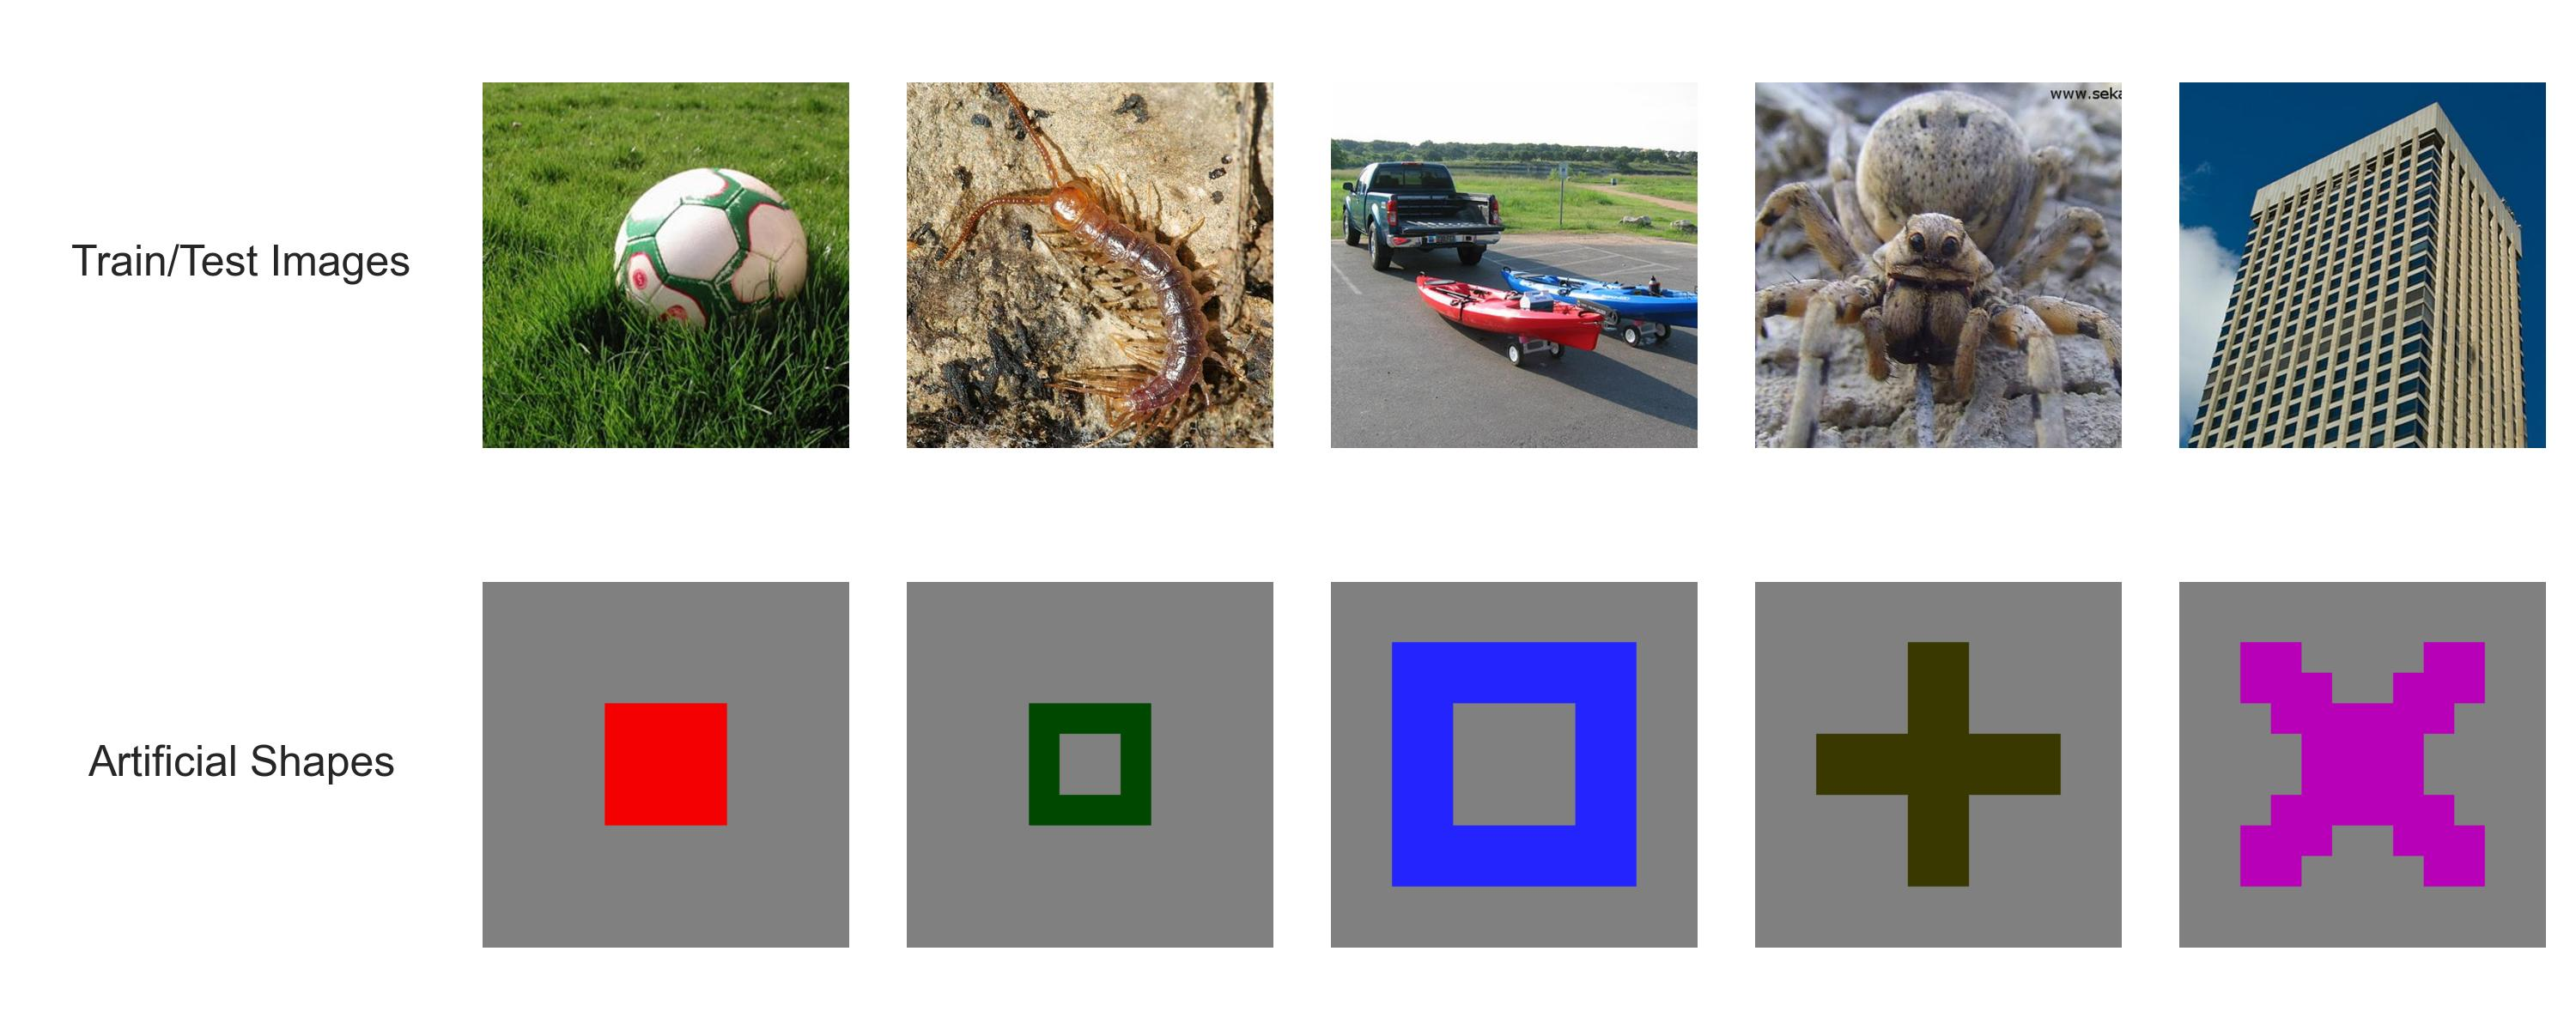
\includegraphics[width=0.8\textwidth]{plots/datasets_train_art_images.jpeg}
    \caption[Selection of natural images and artificial shapes]{\rOne{A selection of natural images (similar in the training dataset and the natural test images) and artificial shapes test images}}\label{fig:datasets_train_art}
\end{figure}

\subsection{MRI data}
% Hier kann ich evtl die Beschreibung aus dem Kamitani Lab nutzen
\subsubsection{MRI data acquisition}
The fMRI data was collected using a 3.0-T Siemens MAGNETOM Verio scanner at the Kyoto University Institute for the Future of Human Society (formerly, Kokoro Research Center). An interleaved T2*-weighted gradient-echo echo-planar imaging scan was performed to acquire functional images covering the entire brain [repetition time (TR), 2000 ms; echo time (TE), 43 ms; flip angle, 80°; field of view (FOV), 192 $\times$ 192 \rOne{mm\textsuperscript{2}}; voxel size, 2 $\times$ 2 $\times$ 2 mm3; slice gap, 0 mm; number of slices, 76; and multiband factor, 4]. T1-weighted (T1w) magnetization-prepared rapid acquisition gradient-echo fine-structural images of the entire head were also acquired [TR, 2250 ms; TE, 3.06 ms; inversion time (TI), 900 ms; flip angle, 9°; FOV, 256 $\times$ 256 \rOne{mm\textsuperscript{2}}; and voxel size, 1.0 $\times$ 1.0 $\times$ 1.0 \rOne{mm\textsuperscript{3}}].

\subsubsection{MRI data preprocessing}
MRI data preprocessing was performed through the pipeline of FMRIPREP (version 1.2.1). For the functional data of each run, a BOLD reference image was first estimated using a custom methodology of FMRIPREP.\@ Then, data were motion-corrected using MCFLIRT from FSL (version 5.0.9) and slice time-corrected using 3dTshift from AFNI (version 16.2.07), based on this BOLD reference image. Next, the corresponding T1w image was coregistered using boundary-based registration implemented by bbregister from FreeSurfer (version 6.0.1). The coregistered BOLD time-series were then resampled onto their original space (2 $\times$ 2 $\times$ 2 \rOne{mm\textsuperscript{3}} voxels) with antsApplyTransforms from ANTs (version 2.1.0) using Lanczos interpolation. After obtaining the resampled BOLD time series, the time series was first shifted by 4 s (two volumes) to compensate for hemodynamic delays, and then nuisance parameters from each voxel’s time series of each run were regressed out, including a constant baseline, a linear trend, and temporal components proportional to the six motion parameters calculated during the motion correction procedure (three rotations and three translations). Single-trial data samples were created by reducing extreme values (beyond ±3 SD for each run) of the time series and averaged within each 8 s trial (four volumes).

\subsubsection{Brain regions of interest}
According to standard retinotopy experiments~\cite{engelFMRIHumanVisual1994,serenoBordersMultipleVisual1995}, V1, V2, V3, and V4 were delineated. The LOC, FFA, and PPA were identified using conventional functional localizers~\cite{kanwisherFusiformFaceArea1997,epsteinCorticalRepresentationLocal1998,kourtziCorticalRegionsInvolved2000}. The higher visual cortex (HVC) region was defined by manually delineating a contiguous region that covered the LOC, FFA, and PPA on the flattened cortical surfaces. The VC was defined by combining V1 to V4 and the HVC.\@ For all the upcoming experiments, the whole VC was used for the reconstruction. After pre-processing the number of Voxels in the VC that can be used for the reconstruction task ranged from 13,135 to 16,667.

% {'S1': 13596, 'S2': 14597, 'S3': 13135, 'S4': 16067, 'S5': 13149, 'S6': 15316}

% Images were collected from an online image database ImageNet31 (2011, fall release), an image database where images are grouped according to the hierarchy in WordNet38. We selected 200 representative object categories (synsets) as stimuli in the visual image presentation experiment. After excluding images with a width or height o100 pixels or aspect ratio 41.5 or o2/3, all remaining images in ImageNet were cropped to the centre.

% Description of fmri-data 
%% Number of subjects
%% Number of runs per image
%% Experimental Design how the participants are shown the images
%% ROI Experiments
%% Chosen ROIs

\section{Reconstruction algorithms}

% How does the whole reconstruction pipeline look like? Both for iCNN and for Brain-Diffuser
In this work, the two algorithms Brain-Diffuser~\cite{ozcelikNaturalSceneReconstruction2023} and iCNN~\cite{shenDeepImageReconstruction2019}, that are described in more detail above, are used. The parameters for the algorithms that are used for this work are stated below. The entire codebase, which this work is based on, is publicly available on github~\cite{mildenbergerDiversity_thesis}, the associated README describes how to work with the codebase. 

\subsection{Brain-Diffuser}
% Brain-diffuser
Unless stated otherwise, the default settings described in the original publication are used for the Brain-Diffuser algorithm. For this purpose, the publicly available codebase~\cite{ozcelikOzcelikfuBraindiffuser2025} was used and adapted so that the Deeprecon data set can also be used.
First, the mean value of the measured brain activity of the 5 image presentations was calculated for each of the 1200 images in the training data set. This data serves as input for both the Brain-Diffuser algorithm and the iCNN algorithm. It should be noted that a better performance in the reconstruction could possibly result if the 5 presentations of each stimulus were included individually in the training data (i.e.\ a total of 6000 training samples are available). Since the main aim of this work is to investigate the relative difference between different test conditions and not to achieve the highest possible absolute performance, it was decided to calculate the mean value of the activation in order to save computing resources.

%% Regression
\subsubsection{Brain-Diffuser translator}
As is usual in reconstruction algorithms, the Brain-Diffuser algorithm first trains \rOne{translator} that map the brain activity into a latent space, which can then be used for reconstruction. There are three different \rOne{translators} that are trained for the Brain-Diffuser: one that maps the brain activity to the latent space of a VDVAE, one for CLIP Text features and one for the CLIP Vision features. The activations of all voxels recorded during the presentation of an image serve as predictor values.

The criteria to be predicted are the embeddings of the stimuli in the respective latent spaces of the three components. These true features must first be extracted from the simulus material. For the VDVAE, the model of Child et al.~\cite{childVeryDeepVAEs2020} is used, which was pre-trained with the ImageNet data set (64 $\times$ 64 pixels). As with the original Brain-Diffuser, only the first 31 layers of the total 75 layers of the VDVAE are used here, as adding further layers would not improve the prediction, but unnecessarily increase the size of the \rOne{translator} module. The 31 VDVAE layers of the embedded training images were concatenated so that the \rOne{translator} has to learn to predict a 91168-dimensional vector. 
Since CLIP~\cite{radfordLearningTransferableVisual2021} is a multimodal model, it can be used to extract both the true features from the presented images (CLIP Vision) and the associated captions (CLIP Text). For this work, a pre-trained CLIP network is used which is based on the Transformer architecture (ViT-L/14). For CLIP Vision, the images are embedded in a space with 257 $\times$ 768 values (256 image patches and a final vector for the entire image). For CLIP Text, the captions are embedded in a space with 77 $\times$ 768 values (76 tokens and a final vector for the entire caption). As 5 different captions were generated for each image, the average value of the latent space from all 5 captions is used as the true feature for CLIP Text.

% Ridge Regression

For the Brain-Diffuser algorithm, the linear ridge regression~\cite{hoerlRidgeRegressionBiased1970} is used for all \rOne{translators}. The ridge regression extends the linear regression by adding a penalty term, which is controlled via the coefficient $\lambda$ and regularizes (i.e.\ shrinks) the estimated coefficients. The higher $\lambda$, the more the parameters are shrunk. Especially in cases where a high dependency between individual predictors is to be expected, more robust parameters can be estimated in that way. Since the activation of neighboring neurons in the visual cortex is usually correlated~\cite{smithSpatialTemporalScales2008}, ridge regression is escpecially helpful in our case.

The ridge regression minimizes the following objective function:
\[
\min_{\beta} \sum_{i=1}^{n} {|y_i - x_i\top \beta|}^2 + \lambda |\beta|^2_F
\]
\noindent{}\rTwo{where \(y_i\) is the extracted \rOne{(true)} feature-vector (VDAVE, CLIP Text or CLIP Vision) for the \(i\)-train image or caption, \(x_i\) is the vector of recorded voxels in response to the \(i\)-th picture, \(\beta\) is the \rOne{matrix} of coefficients to be estimated, and \(\lambda\) is the regularization parameter controlling the strength of the penalty.} For the prediction of the latent space of the VDAVE, $\lambda_{\mathrm{VDVAE}}=50000$ is set, for CLIP Text $\lambda_{\mathrm{CLIP Text}}=100000$ and for CLIP Vision $\lambda_{\mathrm{CLIP Vision}}=60000$.


\subsubsection{Brain-Diffuser reconstruction}
% % Reconstruction
After the brain activity for the test datasets has been mapped to the latent spaces of VDVAE, CLIP Text and CLIP Vision using the \rOne{translators}, these \rOne{translated} features can be fed into the generator in the second step, which reconstructs the images.

% Versatile Diffusion
The Versatile Diffusion Algorithm~\cite{xuVersatileDiffusionText2024} is used as the reconstruction module in the Brain-Diffuser. The model used here was pre-trained on the Laion2B-en~\cite{schuhmannLAION400MOpenDataset2021} dataset. During the reconstruction itself, no parameters are trained, only the pre-trained parameters of the models are used. First, the generator part of the VDVAE is used to generate a first (blurry) approximation of the final reconstructed image from the predicted features. The VDVAE generates images with a size of 64 $\times$ 64 pixels, which are first scaled up to a size of 512 $\times$ 512 to serve as a prior for the Versatile Diffusion Generator. The image generated by the VDVAE adds noise to 37 of the 50 forward diffusion steps. In the backward-denoising process, the generated image is conditioned by both the predicted CLIP Vision (relative strength 0.6) and CLIP Text (relative strength 0.4) features. The generated images have a size of 512 $\times$ 512 pixels. \rThree{It should be noted, that the whole CLIP Vision and CLIP Text embeddings are used and not only the final output vector. Thus the dimensionality of the used CLIP Vision embeddings is 257$\times$768 (256 for all vision transformer patches in the image and one global CLIP vector) and 77$\times$768 for the CLIP Text embeddings (75 tokens and one global CLIP vector)}.

% iCNN
\subsection{iCNN}
Similarly to the brian-diffuser, the iCNN~\cite{shenDeepImageReconstruction2019} algorithm also consists of a \rOne{translator} and a reconstruction module. 
\subsubsection{iCNN \rOne{translator}}
The averaged activations of all voxels are again the predictors for the \rOne{translator}. The criteria are the features of a VGG19~\cite{simonyanVeryDeepConvolutional2014} model, with which the stimuli (resized to 224$\times$224 pixels) are encoded. The VGG19 implementation of PyTorch was used, whereby the weights of the Caffe implementation~\cite{ModelZoo} (pre-trained on ImageNet) were used to create the same conditions as in the original implementation by Shen et al.~\cite{shenDeepImageReconstruction2019}. The features from the 19 layers of the VGG were then reshaped into one-dimensional vectors. As with the Brain-Diffuser, a ridge regression is then also calculated, which predicts the features from the voxel data, the ridge parameter is set to $\lambda=50000$.

\subsubsection{iCNN reconstruction}
Once the brain activity of the test data sets has been mapped to the feature space of the VGG19 layer using the learned regression, the reconstruction of the images with the iCNN algorithm~\cite{shenDeepImageReconstruction2019} begins. First the predicted features ware scaled using the mean and standard deviation of the train images. The implementation of the BdPy package~\cite{KamitaniLabBdpy2024} is used for this (relu7 generator). The SGD optimizer is used and the number of iterations in which the reconstructed image is adapted to the predicted features is set to 500. Normally distributed noise was used as a prior.


\subsection{\rThree{Recovery check}}
\begin{figure}[ht]
    \centering
    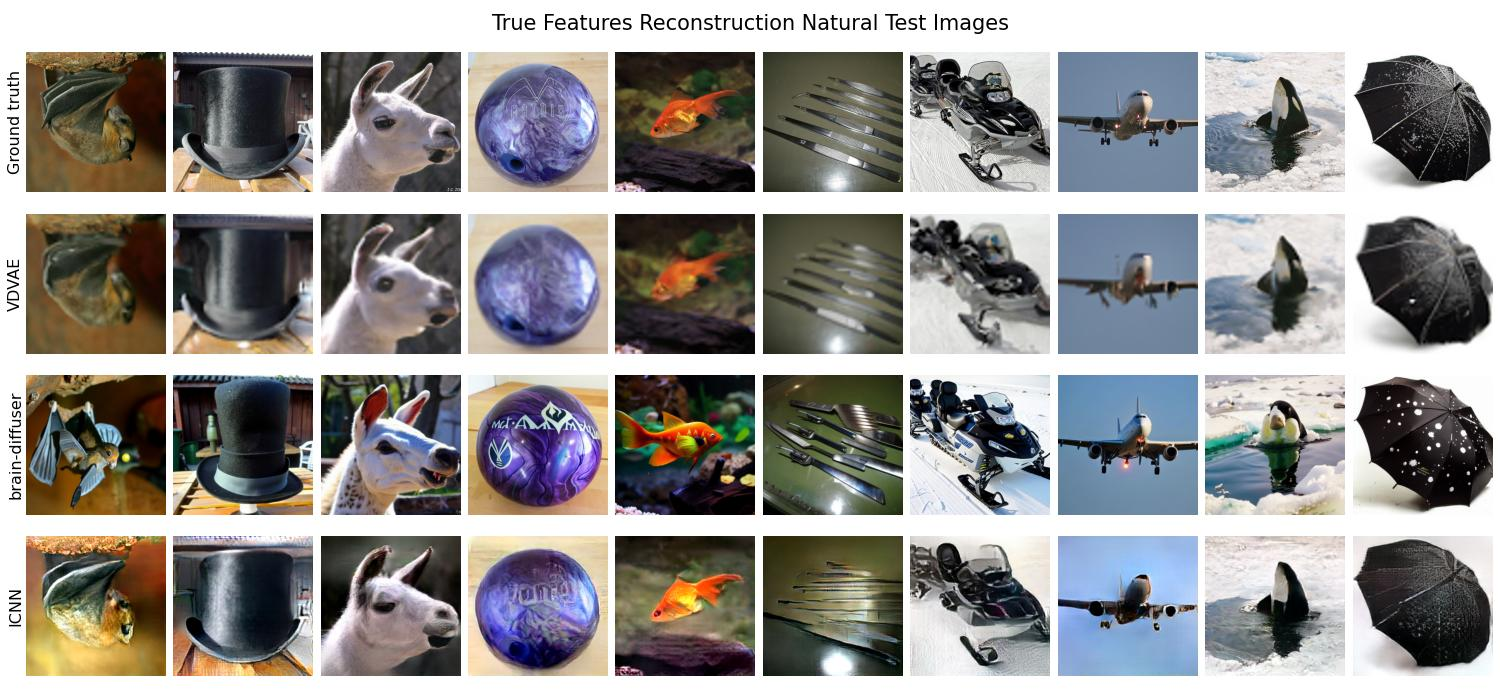
\includegraphics[width=1\textwidth]{plots/baseline_qual_true_recon_test.JPEG}
    \caption[Recovery check]{\rThree{Recovery check} reconstruction for natural test images. \rOne{The top row depicts the ground truth images. Each following row depicts the reconstruction with true features with the algorithm named on the left side.  Note that the VDVAE is only a part of the whole Brain-Diffuser algorithm.}}\label{fig:baselinetruerecon}
\end{figure}
\noindent{}\rOne{To \rThree{verify the} theoretical upper limit for the reconstruction performance of the two algorithms, the true features can be used for reconstruction. \rThree{This procedure is called `recovery check'.} Here, features extracted directly from the stimulus material are fed into the reconstruction module. This means that no brain data is used for the \rThree{recovery check}. It therefore offers the opportunity to see how good the reconstruction could be if the latent features could be perfectly predicted from the brain data.} Figure~\ref{fig:baselinetruerecon} \rOne{shows the recovery check for 10 of the 50 images of the test data set with natural images.}

\rOne{
In the figure, the \rThree{recovery check} is done both for the Brain-Diffuser (the intermediate result of the VDVAE and the final result of the versatile diffusion) and the iCNN algorithms. The first line shows the images that were presented to the test subjects during the experiment. In addition to the final result of the Brain-Diffuser algorithm (shown in the third row), the intermediate result of the VDVAE is also shown in the second row. It can be seen that the VDVAE algorithm shows a \rThree{precise} reconstruction performance for all images and is usually only a slightly blurred image of the ground truth. This is to be expected, as the VDVAE is precisely designed to reconstruct original images from a reduced feature space with as few errors as possible. The final result of the Versatile Diffusion of the Brain-Diffuser algorithm also shows \rThree{high} performance in principle, but it becomes apparent that details from the image are sometimes displayed incorrectly or are hallucinated. For example, the bat looks more like a bird, the fish swims in the wrong direction or additional writing is visible on the sphere. The iCNN algorithm is close to the result of the VDVAE.\ Most of the images can be displayed \rThree{with high quality}. However in particular, details and the coloring of backgrounds  are sometimes incorrectly reconstructed by the iCNN.}
% True-Feature Reconstruction

Figure~\ref{fig:baselinetruerecon_art} \rOne{shows the \rThree{recovery check} for the artificial shapes. The figure can be read in the same way as the previous one. Here we can also see that \rTwo{on the one hand,} the iCNN in general can also predict the shape of the images \rThree{with high accuracy}, \rTwo{on the other hand} it becomes especially visible that the colors of the backgrounds can not always be reconstructed properly, since most of the reconstructed images have an almost white background even though it should be dark grey. The Brain-Diffuser shows again some hallucinations, for example an additional circle has appeared around the blue cross.}

\rOne{In summary, the recovery check shows that both algorithms are basically capable of reconstructing images from a feature space, even if both algorithms have some weaknesses for either colors or details of the reconstructed images.}

\begin{figure}[ht]
    \centering
    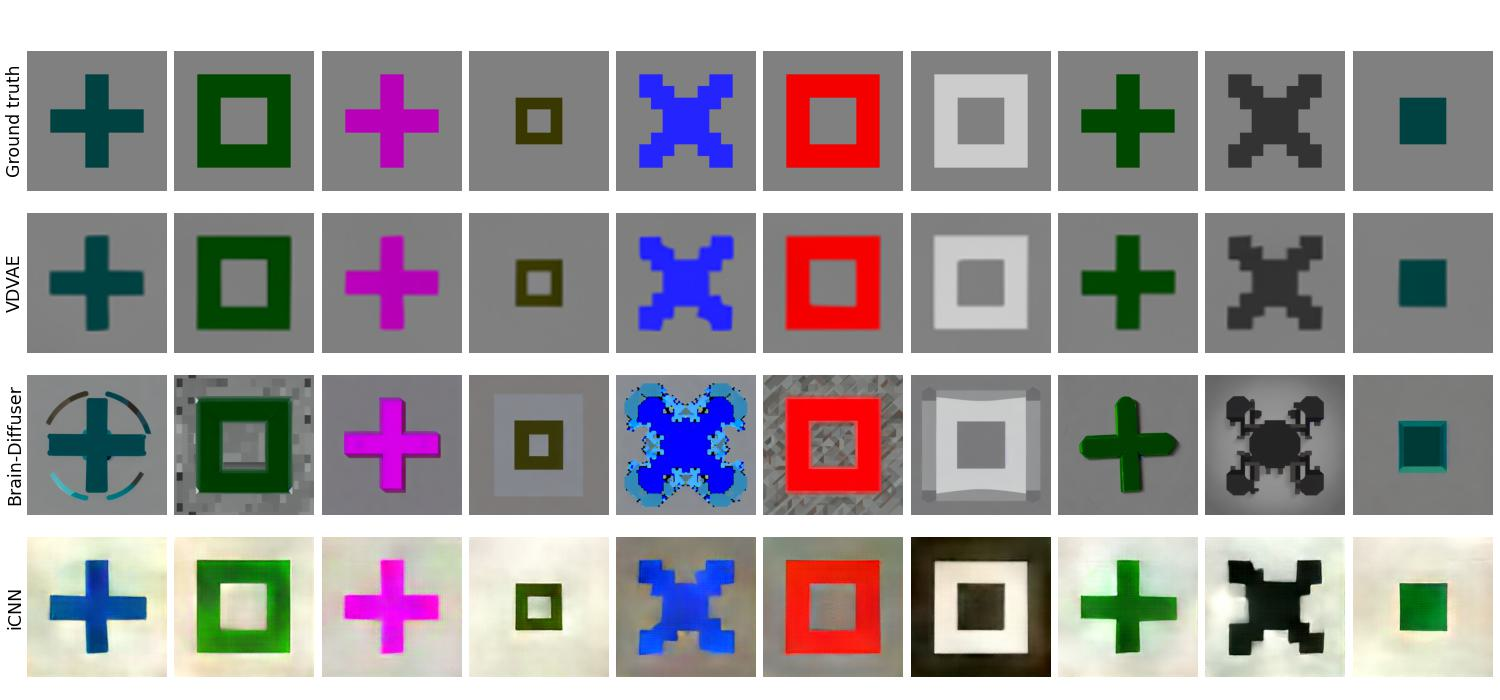
\includegraphics[width=1\textwidth]{plots/baseline_qual_true_recon_art.JPEG}
    \caption[Recovery check for artificial shapes]{Recovery check for artificial shapes. \rOne{The top row depicts the ground truth image. Each following row depicts the reconstruction with true features with the algorithm named on the left side. Note that the VDVAE is only a part of the whole Brain-Diffuser algorithm.}}\label{fig:baselinetruerecon_art}
\end{figure}

% Small Evaluation of the True-Feature Reconstruction

\section{Evaluation metrics}
%% Regression Criteria
% Profile Correlation
% Pattern Correlation
% Pairwise Identification Accuracy

It is possible to evaluate both stages of the reconstruction algorithms (the \rOne{translation} and the reconstruction). The results of the regressions are used to evaluate the \rOne{translation} part of the algorithms and the final reconstructed images are examined to evaluate the reconstruction part of the algorithms. \rOne{Each presentation of an image for a subject is treated as an independent sample. The data from the different subjects is interpreted as a unit for replicating the experiment to investigate the robustness of the results. Thus the data will not be pooled across the subjects and statistical tests will not be executed.} Thus, even though quantitative metrics are computed, they will be evaluated in a rather qualitative way by referring plots and interpreting the results.


\subsection{Measuring \rOne{translation} performance}
\rOne{To evaluate the translation performance, pairwise identification accuracy will be used}. The pairwise identification accuracy is a metric frequently used to determine the feature prediction in reconstruction algorithms~\cite{shirakawaSpuriousReconstructionBrain2024}. 
The pairwise identification accuracy measures whether a predicted feature vector is more similar to the true feature than the other predicted vectors. For a feature vector $i$, it is defined as:


\[ % Only for image i
\text{PairwiseIDAcc}_i \coloneq \frac{1}{n-1} \sum_{\substack{j=1 \\ j \neq i}}^{n} \mathbb{I} \left(  \text{sim}\left(\hat{y}_{i}, y_{i}\right)  > \text{sim}\left(\hat{y}_{j}, y_{i} \right) \right)
\]
\noindent{}\rTwo{where \( y_{i} \) represents the true feature vector for the \( i \)-th sample, \( \hat{y}_{i} \) represents the predicted feature vector for the \( i \)-th sample, \( \text{sim}\left( \cdot, \cdot \right) \) denotes an arbitrary distance metric for vectors and \( \mathbb{I}(\cdot) \) is the indicator function, which equals 1 if the condition inside is true and 0 otherwise.} The \rOne{similarity} metric can be freely chosen, in this work, the cosine \rOne{similarity} is used, since the high dimensionality negatively affects the euclidean distance~\cite{koppen2000curse}. The cosine \rOne{similarity} between to vectors \textbf{a} and \textbf{b} is calculated as follows:

\[
\text{cosine\_sim}(a, b) \coloneq \frac{a \cdot b}{\|a\| \, \|b\|}
\]

\noindent{}If a feature vector cannot be predicted from brain activity, one would expect the pairwise identification accuracy to be 0.5, since it will be a matter of chance whether any other vector is  more or less similar to the true feature than the actually predicted feature vector. In order to compute the Pairwise Identification Accuracy, for the different \rOne{translators} of the iCNN and the Brain-Diffuser, the corresponding multidimensional feature vectors are reshaped to a one-dimensional vector to be able to compute the vector similarity between layers (for example the convolutional layers of the VGG19 are multidimensional). \rOne{The pairwise identification may be abbreviated as ID Accuracy in the following}. 


\subsection{Measuring reconstruction performance}

The final results of the reconstruction algorithms can in turn be analysed both qualitatively and quantitatively. Different metrics can be used to compare the ground truth images and the reconstructed images on a quantitative level~\cite{ozcelikNaturalSceneReconstruction2023}. On the one hand, the metrics can focus on the low-level features of an image (e.g.\ structure and colour); on the other hand, there are metrics that compare the high-level features of the images (i.e.\ the semantic meaning). For an appropriate judgement on the overall quality of a reconstruction, it is important to consider both the low-level and high-level features (a reconstructed image that has the correct outlines but completely ignores the semantic concepts is just as bad as an image in which the meaning has been correctly captured but the position and position of the objects in the image are incorrectly represented).

In this work, the PixelCorrelation is used as a low-level metric~\cite{shenDeepImageReconstruction2019,ozcelikNaturalSceneReconstruction2023}. In this method, the reconstructed images and the ground truth image are first reshaped into a one-dimensional vector and the correlation between the two is then calculated. The expected value for random reconstructions would be $r=0$. \rOne{The PixelCorrelation may be abbreviated with PixCorr in some plots}.

\rOne{CLIP-accuracy measures the semantic (high-level) similarity between reconstructed images and ground truth images by embedding both into a shared semantic feature space using a CLIP Vision encoder~\cite{radfordLearningTransferableVisual2021}. To align with the evaluation methodology of Brain-Diffuser~\cite{ozcelikNaturalSceneReconstruction2023} and ensure comparability with their results, this study adopts the same approach. This metric quantifies how frequently the embedded semantic features of correctly matched image pairs (each reconstructed image with its corresponding ground truth) show higher correlation compared to incorrectly matched pairs (a reconstructed image with a non-corresponding ground truth). Thus this metric is very similar to the pairwise identification accuracy that was described above, only that it is comparing the results in the CLIP feature space. The random chance-level baseline for this metric is again 0.5. \rTwo{To} make the CLIP-accuracy results more directly comparable in scale to other metrics used in this thesis, the random baseline value of 0.5 is subtracted from the raw accuracy scores. Consequently, the adjusted CLIP-accuracy presented here has a random-chance baseline of 0 and a theoretical maximum of 0.5. The CLIP-accuracy may be abbreviated with CLIP-acc in some plots.}

In addition to the low-level and high-level differences, a third quantiative metric is used in this work to test the reconstruction performance. Since the natural human judgement about the similarity of images is based on several visual attributes that integrate low-level features with high-level features~\cite{sundaramWhenDoesPerceptual2024}, DreamSim~\cite{fuDreamSimLearningNew2023} was developed to get closer to the natural judgement about the similarity of images. DreamSim combines various image features and has been fine-tuned with human judgement to better estimate the ``mid-level'' similarity between images. To calculate the similarity between two images, the cosine-similarity (i.e.\ 1\@ $-$\@ cosine distance) between the DreamSim embedding vector of the ground truth and the predicted image is calculated. In a random reconstruction, the cosine similarity would be 0 (the feature vectors are be orthogonal to each other). \rOne{Note that the cosine distance may be abbreviated as cos\_dist in some plots.}

Since even the DreamSim metric is not perfect for comparing the similarity of images, and since judgments of quality may vary from person to person, the differences are also described qualitatively. Individual examples of the actual reconstructed images are shown and compared to the ground truth images for each test condition tested in this paper.

\section{Baseline results}
In order to validate the reconstruction algorithms used in this work, the results of the two algorithms are presented below. No other changes were made to the input datasets or the method, so the results can be used as a baseline for comparison with the further results of the following experiments.

\subsection{\rOne{Translation} results}
\rOne{Figure~\ref{fig:baselinetranslator} shows the results for the \rThree{translator}. The mean values over all 50 (natural test images) or 40 (artificial images) test samples are shown. The error bars are the standard errors. From now on, all error bars in this study will be standard errors over the 50 (or 40 respectively) test images unless reported otherwise. All mean values for all participants are clearly above the random probability of 0.5. Thus, for both the Brain-Diffuser and iCNN, the \rOne{translators} have the ability to predict the true features of the test images to some extent. The performance is also relatively constant across the different subjects, with the significantly larger differences being found between the different \rOne{translator} modules. In particular, for the CLIP Text features, the identification accuracy is very high at 0.892 on average and is already close to the upper limit of 1.0. \rThree{For the artificial shapes,} a slightly different picture emerges in contrast to the natural test images. Here, \rOne{translator} has to generalise outside its training domain. All individual values are lower than with the natural test images. iCNN (from 0.831 to 0.782) and VDVAE (from 0.761 to 0.665) show only a comparatively small drop in performance. For the two CLIP \rOne{translator}, the difference to the natural test images is significantly greater (CLIP Vision falls from 0.777 to 0.54 and CLIP Text falls from 0.892 to 0.558). The identification accuracy for the CLIP \rOne{translators} is only just above the chance probability of 0.5 for the artificial test images.}

% In addition, the results aggregated over all 5 subjects for both types of test images are listed in Table~\ref{tab:baseline_translator}, with the standard deviation in parentheses.


\begin{figure}[ht]
    \centering
    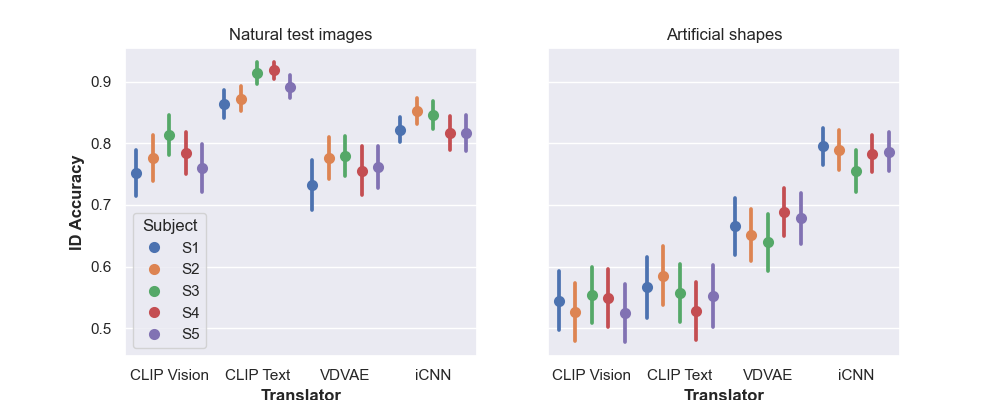
\includegraphics[width=1\textwidth]{plots/baseline_translator.png}
    \caption[Translator performance baseline]{\rOne{Translator} performance for the Brain-Diffuser and iCNN on natural test images and artificial shapes. \rOne{The identification accuracy of all four translators (the three translators for VDVAE, CLIP Text and CLIP Vision from the Brain-Diffuser and the translator for the iCNN) is depicted for each of the five subjects. The standard error across all test samples is depicted in the error bars.}}\label{fig:baselinetranslator}
\end{figure}


% \begin{figure}[ht]
%     \centering
%     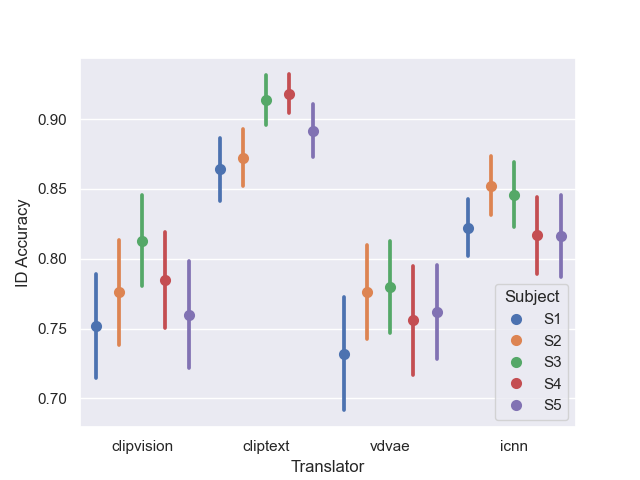
\includegraphics[width=0.6\textwidth]{plots/baseline_translator_test.png}
%     \caption[Translator performance natural test images baseline]{\rOne{Translator} performance for the Brain-Diffuser and iCNN on natural test images. \rOne{The identification accuracy of all four translators (the three translators for VDVAE, CLIP Text and CLIP Vision from the Brain-Diffuser and the translator for the iCNN) is depicted for each of the five subjects. The standard error across all test samples is depicted in the error bars.}}\label{fig:baselinetranslatortest}
% \end{figure}

% \begin{figure}[ht]
%     \centering
%     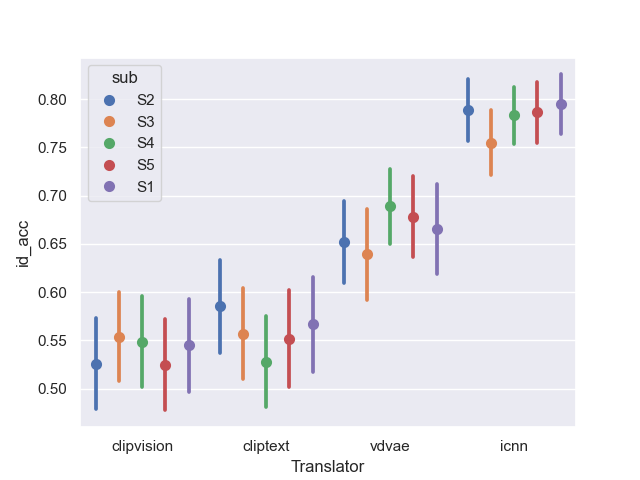
\includegraphics[width=0.6\textwidth]{plots/baseline_translator_art.png}
%     \caption[Translator performance artificial shapes baseline]{\rOne{Translator} performance for the Brain-Diffuser and iCNN on artificial shapes. \rOne{The identification accuracy of all four translators (the three translators for VDVAE, CLIP Text and CLIP Vision from the Brain-Diffuser and the translator for the iCNN) is depicted for each of the five subjects. The standard error across all test samples is depicted in the error bars.}}\label{fig:baselinetranslatorart}
% \end{figure}

% \begin{table}[ht]
%     \centering
% \begin{tabular}{lllll}
\toprule
 & clipvision & cliptext & vdvae & icnn \\
test images &  &  &  &  \\
\midrule
natural & 0.777 (.024) & 0.892 (.024) & 0.761 (.019) & 0.831 (.017) \\
artificial & 0.54 (.013) & 0.558 (.021) & 0.665 (.02) & 0.782 (.016) \\
\bottomrule
\end{tabular}

% \caption{A nice table.}\label{tab:baseline_translator}
% \end{table}


\subsection{Reconstruction results}
\rOne{Ten of the reconstructed images are shown for the natural test images in Figure~\ref{fig:baselinerecontestqual} 
As with the true-feature reconstruction, both the intermediate result of the VDVAE and the overall result are shown here for the Brain-Diffuser algorithm. The VDVAE and iCNN tend to produce blurred outlines, while the Brain-Diffuser algorithm usually creates photorealistic objects. For the natural test images, the VDVAE and iCNN usually \rOne{translate} the outlines approximately correctly. For example, the ball produces a round object in front of a neutral background and the goldfish is reconstructed as a red, elongated object in front of a dark background. The VDVAE produced artefacts for the aeroplane, which could be the result of clipping in the prediction (the predicted values of the features are too high or too low and distort the pixel value). All in all, the results of the VDVAE and iCNN are comparable. The full Brain-Diffuser algorithm is designed to add semantic information to the results of the VDVAE and incorporate this into a photorealistic image with the versatile diffusion process. In the case of natural test images, it looks as if this is at least partially successful: the images that represent living beings (bat, llama, goldfish or orca) also look as if something alive is to be represented in the reconstructed version (even if the exact animal cannot be recognised). Likewise, the inanimate objects (e.g.\ the hat, the surgical instrument or the umbrella) are also reconstructed in a comparatively neutral way. Even the snowmobile looks like a vehicle (with handlebars and wheels) after reconstruction. Only in the case of the aircraft is the interpretation difficult, but this may also be due to the faulty result of the VDVAE.\@ The reconstructed artificial shapes are displayed in Figure~\ref{fig:baselinereconartqual}. The figure follows the same structure as before.The VDVAE and iCNN are again largely able to reconstruct the correct shapes for the here. Only the shape `X' cannot be reconstructed very well. As the results of the \rOne{translator} already indicated, the final Brain-Diffuser result for the artificial shapes is far from perfect. Here, too, photorealistic images are usually generated. The shapes are often well adopted by the VDVAE and then converted into a photorealistic image with false details hallucinated by the diffusion algorithm (for example, in the image with the purple cross on a person can be seen).}

The plot in Figure~\ref{fig:baselinereconquant} shows the results of the quantitative evaluation of the image reconstruction for the individual subjects. As with the \rOne{translators}, the error bars are the standard errors. The three previously described measurement parameters, PixelCorrelation, DreamSim-distance and CLIP-accuracy, are shown for the iCNN and Brain-Diffuser (bd) algorithms. For the natural test images, \rOne{there is only a slight difference between iCNN and Brain-Diffuser in terms of DreamSim (iCNN has a slightly higher DreamSim than Brain-Diffuser)}. In terms of CLIP accuracy, however, the reconstructions of the Brain-Diffuser show consistently higher performance than the iCNN.\@ The difference in the pixel correlation is not as visible in the graphic, but it appears that the iCNN consistently achieves higher results in this low-level metric than the Brain-Diffuser. \rThree{For the artificial shapes}, as with the \rOne{translator}, the results are \rOne{in general} less accurate than for the natural images. The iCNN now clearly performs better than the Brain-Diffuser in terms of both the DreamSim-distance and the pixel correlation. For the CLIP accuracy \rOne{(where before the Brain-Diffuser performed better than iCNN)}, there is no longer any \rOne{visible} difference between the two algorithms, and the results are very close to the random probability of 0.5. 


\begin{figure}[ht]
    \centering
    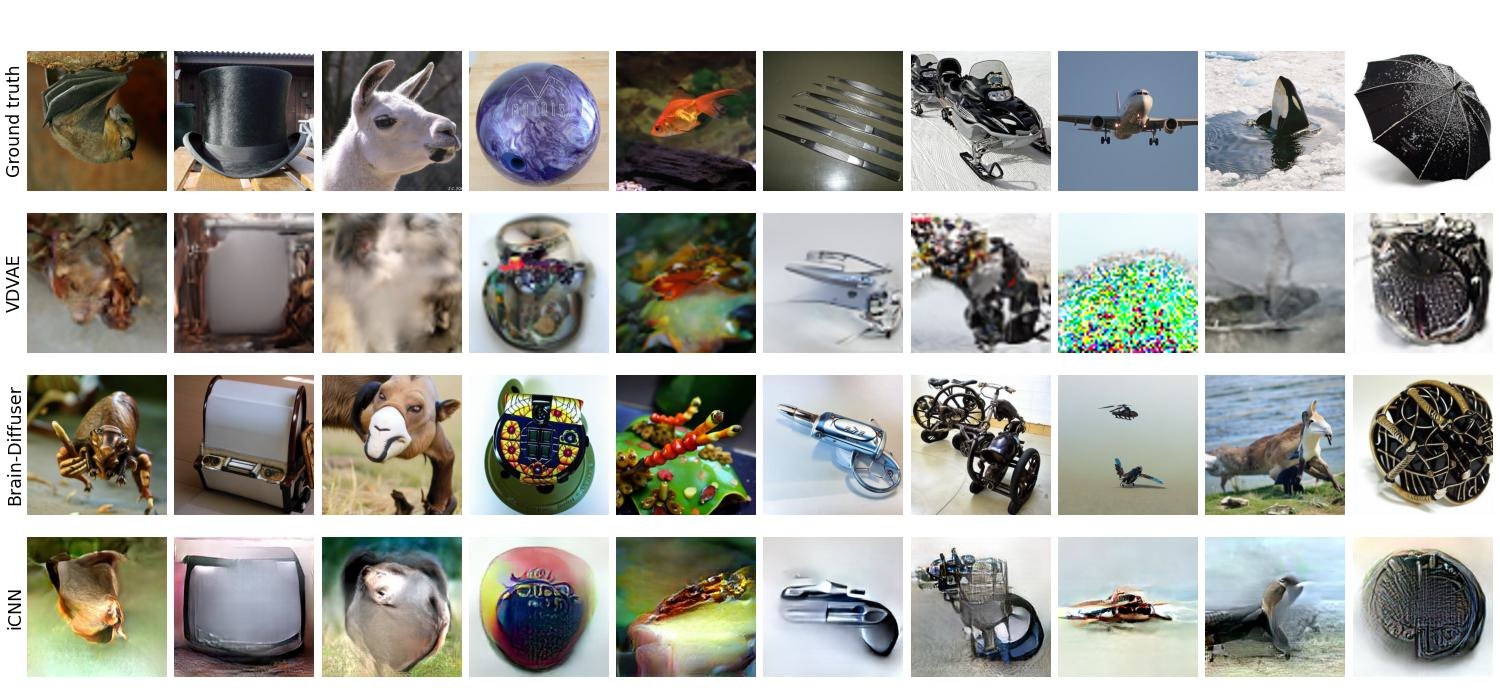
\includegraphics[width=1\textwidth]{plots/baseline_qual_recon_test.JPEG}
    \caption[Reconstructed images for iCNN and Brain-Diffuser on natural test images]{Qualitative results of iCNN and Brain-Diffuser on natural test images. \rOne{The top row depicts the ground truth image. Each following row depicts the reconstruction from the predicted features with the algorithm named on the left side. Note that the VDVAE is only a part of the whole Brain-Diffuser algorithm.}}\label{fig:baselinerecontestqual}
\end{figure}

\begin{figure}[ht]
    \centering
    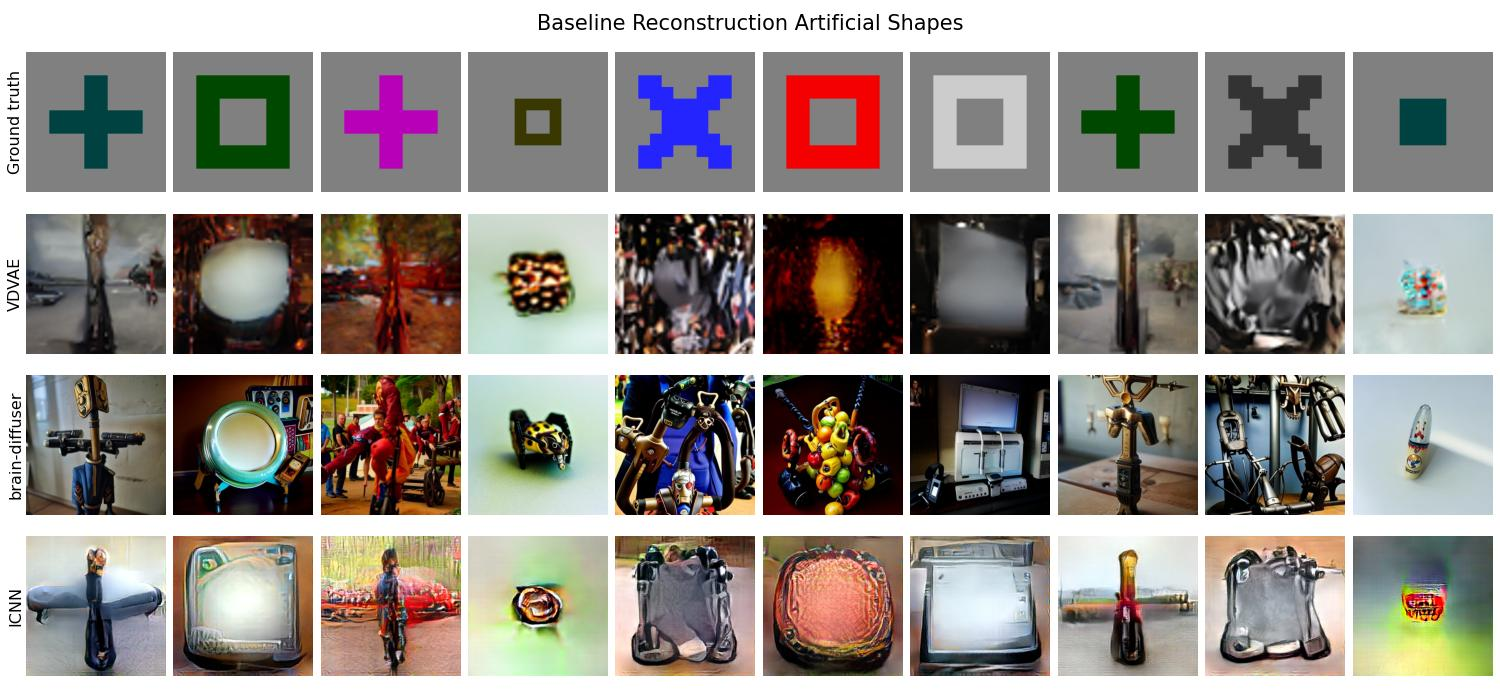
\includegraphics[width=1\textwidth]{plots/baseline_qual_recon_art.JPEG}
    \caption[Reconstructed images for iCNN and Brain-Diffuser on artificial shapes]{Qualitative results of iCNN and Brain-Diffuser on artificial shapes. \rOne{The top row depicts the ground truth image. Each following row depicts the reconstruction from the predicted features with the algorithm named on the left side. Note that the VDVAE is only a part of the whole Brain-Diffuser algorithm.}}\label{fig:baselinereconartqual}
\end{figure}


\begin{figure}[ht]
    \centering
    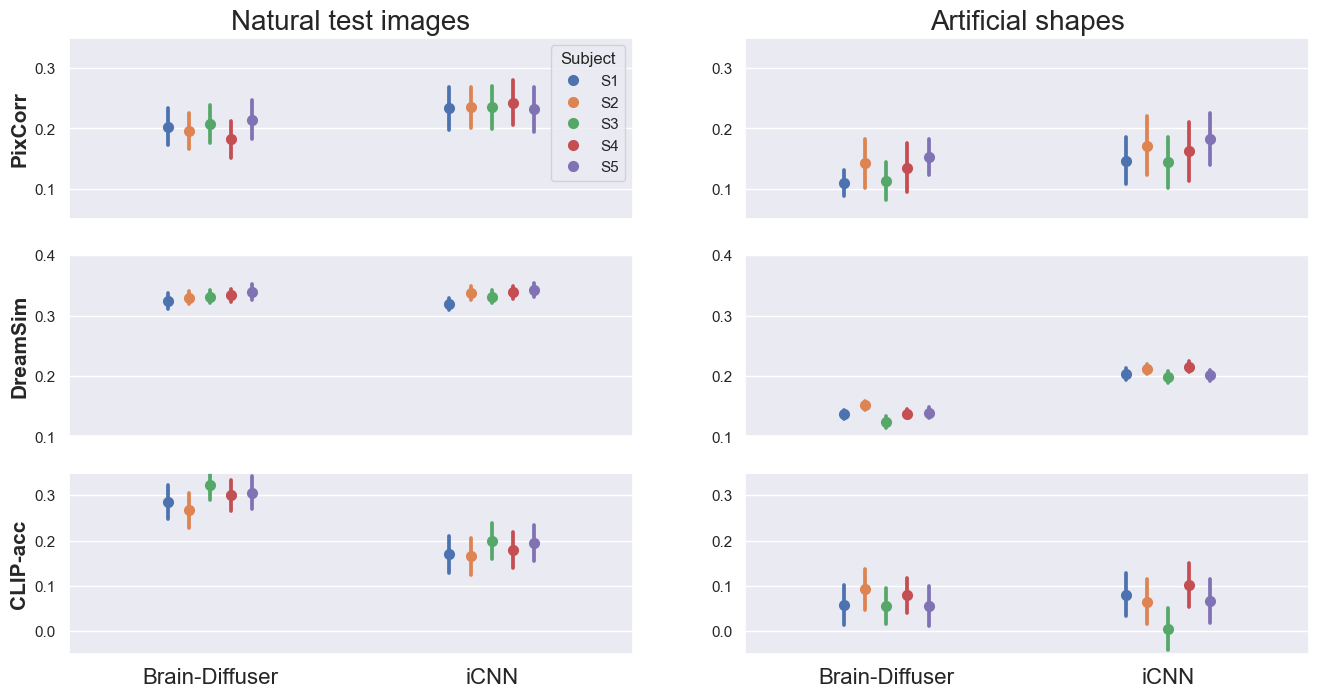
\includegraphics[width=1\textwidth]{plots/baseline_reconstruction.png}
    \caption[Reconstruction performance baseline]{Reconstruction performance of iCNN and Brain-Diffuser. \rOne{For each of the five subjects, the three reconstruction criteria (PixelCorrelation, DreamSim and CLIP-accuracy) are displayed for both the Brain-Diffuser and iCNN algorithm. The errorbars are computed as the standard error across all the test samples.}}\label{fig:baselinereconquant}
\end{figure}

% \begin{figure}[ht]
%     \centering
%     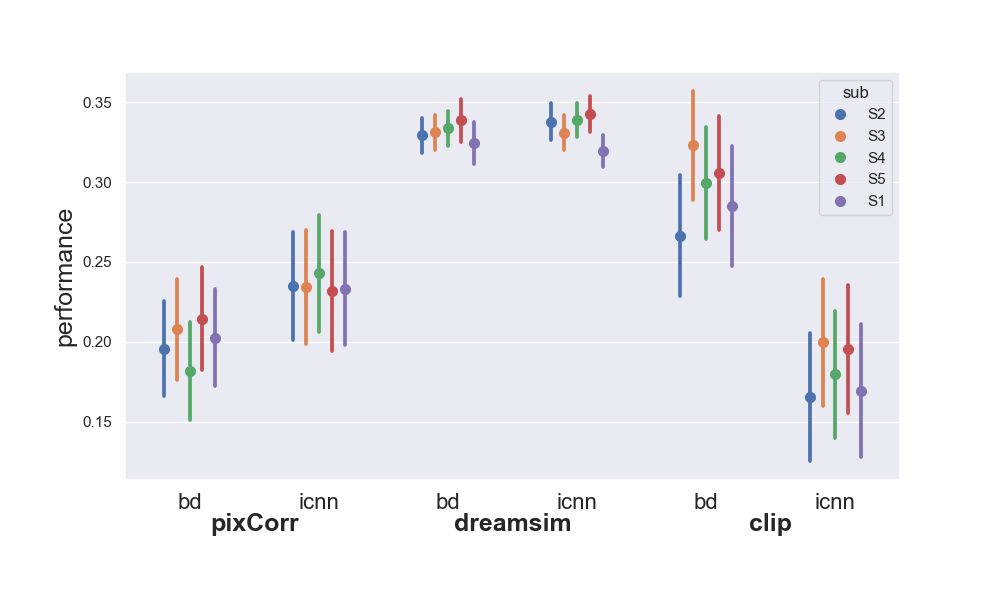
\includegraphics[width=0.8\textwidth]{plots/baseline_reconstruction_test.png}
%     \caption[Reconstruction performance natural test images baseline]{Reconstruction performance of iCNN and Brain-Diffuser on natural test images. \rOne{For each of the five subjects, the three reconstruction criteria (PixelCorrelation, DreamSim and CLIP-accuracy) are displayed for both the Brain-Diffuser and iCNN algorithm. The errorbars are computed as the standard error across all the test samples.}}\label{fig:baselinerecontestquant}
% \end{figure}

% \begin{figure}[ht]
%     \centering
%     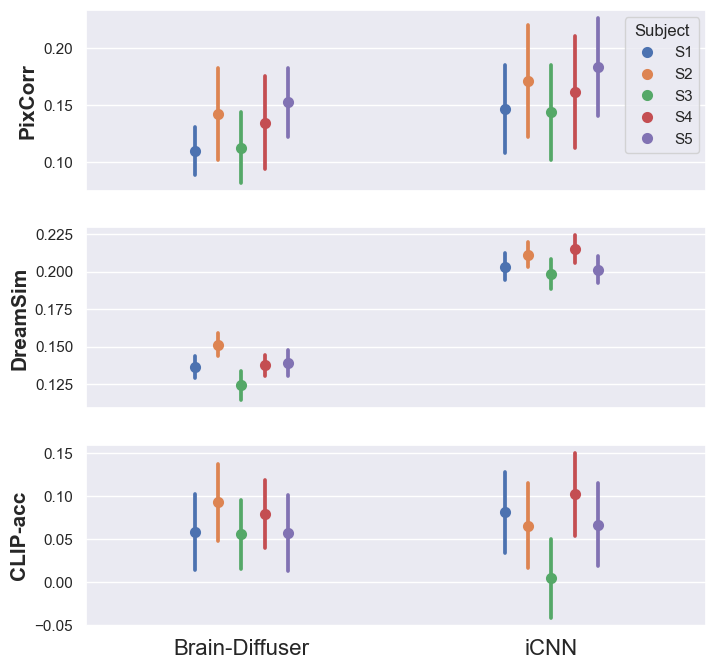
\includegraphics[width=0.8\textwidth]{plots/baseline_reconstruction_art.png}
%     \caption[Reconstruction performance artificial shapes baseline]{Reconstruction performance of iCNN and Brain-Diffuser on artificial shapes. \rOne{For each of the five subjects, the three reconstruction criteria (PixelCorrelation, DreamSim and CLIP-accuracy) are displayed for both the Brain-Diffuser and iCNN algorithm. The errorbars are computed as the standard error across all the test samples.}}\label{fig:baselinereconartquan}
% \end{figure}

% \begin{table}[ht]
%     \centering
% \begin{tabular}{lllll}
\toprule
 &   & pixCorr & dreamsim & clip \\
test images & algorithm &  &  &  \\
\midrule
\multirow[t]{2}{*}{natural} & icnn & 0.235 (.004) & 0.334 (.009) & 0.682 (.015) \\
 & bd & 0.201 (.013) & 0.332 (.005) & 0.796 (.021) \\
\cline{1-5}
\multirow[t]{2}{*}{artificial} & icnn & 0.161 (.017) & 0.206 (.007) & 0.564 (.036) \\
 & bd & 0.13 (.019) & 0.138 (.01) & 0.568 (.017) \\
\cline{1-5}
\bottomrule
\end{tabular}

% \caption{A nice table.}\label{tab:baseline_reconstruction}
% \end{table}

\subsection{Conclusion}
The effectiveness of the two algorithms, Brain-Diffuser and iCNN, could be validated with the Deeprecon data set. It was shown that the \rOne{translator} modules of the algorithms were able to predict the features from the brain activity well above the random probability. Furthermore, it was shown that the reconstructed images also show strong similarities to the ground-truth images, so it is possible to a certain degree to reconstruct seen images from brain activity using the mentioned algorithms. The reconstructed images also look qualitatively similar to those in the relevant literature (see~\cite{shenDeepImageReconstruction2019, shirakawaSpuriousReconstructionBrain2024, ozcelikNaturalSceneReconstruction2023}).
In contrast to the original study, the Brain-Diffuser was evaluated with the Deeprecon dataset and not the NSD dataset. As already described, there is a partial overlap of semantic concepts between the training and the test dataset in the NSD dataset. Accordingly, the results of the Brain-Diffuser in our validation are worse than for the original author~\cite{ozcelikNaturalSceneReconstruction2023}. With our data, the Brain-Diffuser algorithm achieves a PixelCorrelation of 0.201 (0.305 for the original authors) and a CLIP-accuracy of 0.796 (0.925 for the original authors). In particular, the high difference in CLIP accuracy is to be expected, since the semantic overlap between training and test data in the NSD dataset enables the semantic categories to be learned. Thus, the CLIP \rOne{translators} do not need to learn a regression on the complete possible CLIP space, but only needs to perform a classification (generalisation over unknown classes is not fully possible). 
Nevertheless, our results with the Deeprecon data set showed that at least parts of the semantic meaning of the images could be captured (e.g.\ living vs.\ inanimate objects). At least for the natural test data, it has been shown that the iCNN algorithm is better able to reconstruct the low-level structure of an image (difference of PixelCorrelation), while the Brain-Diffuser is better able to recognise high-level concepts (difference of CLIP-accuracy). 
The artificial shapes were consistently  reconstructed worse than the natural test images. This indicates the additional difficulty of out-of-distribution generalisation. Compared to Brain-Diffuser, the iCNN algorithm has lost significantly less in its reconstruction quality. This can be explained by the fact that iCNN is less dependent on learned categories than Brain-Diffuser and thus generalises more easily. The Brain-Diffuser shows the significantly poorer generalisation described by Shirakawa et.\ al.~\cite{shirakawaSpuriousReconstructionBrain2024} The main cause for this is described as output dimension collapse: the \rOne{translator} modules have not been trained with sufficiently diverse data and therefore map to the semantic space known from the training, in which potential (previously unknown) dimensions in the test data set cannot be mapped. To improve the generalisation of the algorithms, it is therefore necessary to have more diverse data in the training set to enable regression into dimensions not present in the training. In the following, we will thus investigate in different experiments what influence the diversity of the training data has on reconstruction and out-of-distribution generalisation, and how the diversity of existing data sets can presumably be increased. 

 \chapter{Experiments}

\section{Experiment 1: Reducing training data with care}

% Corresponding Progress Reports
% https://www.notion.so/241122-Matthias-first-exploration-for-image-dropout-ccb558156ba04efab6435b0f42021d44
% https://www.notion.so/241129-Matthias-Dropout-experiment-first-results-dac4111347ec413c87bbdfdaf4ef495e?pvs=23
% https://www.notion.so/241213-Matthias-iCNN-in-image-dropout-9e810b27443c400f902e232cf966004d?pvs=23
% https://www.notion.so/241220-Matthias-reducing-train-data-with-care-First-AI-captions-0a0a3c610dba4d9c84d4eda4fb1c53dd?pvs=23
% https://www.notion.so/20250117-Matthias-Filling-the-gaps-1-7126a49b2ee34921aff7e853c3a1542c?pvs=23
% https://www.notion.so/Matthias-Mildenberger-243a8aff9cee491a987bc227e5c937cc?p=ef08526d469548adbeedae4384177db1&pm=s
% https://www.notion.so/250214-matthias-filling-the-gaps-4-197726ec52d680a28b00db7958f00613?pvs=23

\subsection{Background}

\rTwo{
As established earlier, the diversity of training data may play a crucial role in determining the performance of brain activity reconstruction. In this first experiment we investigate how different aspects of data diversity ranging from low-level features (such as colors and shapes) to high-level features (such as semantic concepts) influence the image reconstruction from brain activity. Since increasing the data diversity by recording new data is very resource-intensive (recording new data takes time and money), we take a backward approach: we reduce the training data in a strategic way. The reduction will be performed under different subsampling criteria, which relate to different aspects of data diversity (ranging from low-level to high-level features). The aim is to find a way to reduce the training data that allows a reconstruction performance similar to the full data set. This will allow a first exploration of what aspects should be considered when creating a possible new training data set with maximized diversity, that could achieve the best possible results in future new experiments where new brain activity can also be recorded.}

Many studies have explored how to achieve comparable results with reduced training data sets as with the full data set. Wang et al.~\cite{wangDataDropoutOptimizing2018} used a two-step procedure, first training the model on the full training data and then using the validation data to delete any training samples that would reduce the overall loss on the validation data set. This allowed them to remove unfavourable training samples and to end up training a new model on a reduced dataset, which actually performed better than the full dataset. Sener et al.~\cite{senerActiveLearningConvolutional2018} were able to use a core set approach in active learning to ensure that the data selected during model training yield the greatest improvement, thus achieving good classification even with greatly reduced datasets. They were able to outperform many other algorithms and a random subselection baseline. In a detailed review, Guo et al.~\cite{guoDeepCoreComprehensiveLibrary2022} compared different approaches to core set selection, highlighting in particular that random subselection is still a very strong baseline, often outperforming many sophisticated core set approaches. In a dataset for medical imaging of the heart, Kolluru et al.~\cite{kolluruLearningFewerImages2021} were able to reduce the data to almost a tenth of its original size and still achieve acceptable results. They first used an autoencoder to map the images into an abstract feature space, then used PCA to further reduce the dimensionality, and finally used the k-medoids algorithm to form as many clusters in the reduced space as there were images to be extracted from the dataset. In summary, guided reduction of training data is a promising approach to achieving stable performance with significantly fewer resources during training (and presumably data collection).

\rTwo{Various approaches can be used to create subsamples based on maximising the diversity of different features. To create subsamples that maximize the diversity of low-level features (colours, shapes, textures) simple approaches for example based on the distribution of colours in an image~\cite{maheshwariImageClusteringUsing2009} could be used. More sophisticated approaches that can also cover mid-level and high-level features of images may use the activation of pre-trained deep learning models to embed images in a more abstract feature space. In this space semantic clustering becomes possible~\cite{chang2017deep}. Birdokar et al.~\cite{birodkarSemanticRedundanciesImageClassification2019} use different feature layers of a CNN to perform image clustering at different levels (low, mid and high level features). The late layer was especially useful for extracting the semantic features of the images and clustering was used to remove redundant samples. To make clustering algorithms such as k-means computationally feasible, the data from the extracted features should be reduced in dimensionality fist. UMAP~\cite{mcinnesUMAPUniformManifold2018} is a modern nonlinear dimensionality reduction algorithm. In order to cluster the images in a low-level space, UMAP can also be applied directly to the images without first embedding them in a feature space. After the dimensionality reduction, the subsampled datasets can be generated by using clustering such as k-means.}

With respect to \rOne{translating} brain activity, it has been previously found that different levels of the visual system are also better at predicting different feature levels (i.e., low-level brain structures such as V1 and V2 are more suited for predicting low-level features, and high-level structures such as PPA and FFA can predict high-level features)~\cite{horikawaGenericDecodingSeen2017}. However, to the best of our knowledge, there has been no systematic investigation of how maximising the diversity of training data at different feature levels (low-level vs.\ high-level) affects the \rOne{translation} of brain data and the subsequent reconstruction of images. In other words, whether it is more important to have a training set that contains as many different semantic concepts as possible, or to use a training set that contains as many different low-level features (e.g.\ colours and shapes) as possible. 

\rTwo{Building on these considerations, we hypothesize that the feature level at which training data diversity is maximised will directly influence reconstruction performance on test data. Specifically, we expect that the \rOne{translation} and reconstruction of artificial shapes will benefit most from emphasizing low-level feature diversity, as these images are predominantly defined by basic visual attributes such as shape and color. Conversely, reconstruction performance on natural images should improve when prioritizing high-level diversity, since accurate predictions depend on capturing semantic concepts. Additionally, we hypothesize that a balanced, mid-level approach that integrates both low-level and high-level diversity will yield the best overall performance across both image categories. To test the effectiveness of these diversity-based strategies, we include random subselections of the training data as baselines.}


\subsection{Methods}

The procedure for obtaining a reduced training data set with maximised diversity is described below. \rThree{An overview of the whole pipeline and goal for this experiment is is depicted in Figure~\ref{fig:dropout_pipeline}.}

\begin{figure}[ht]
  \centering
  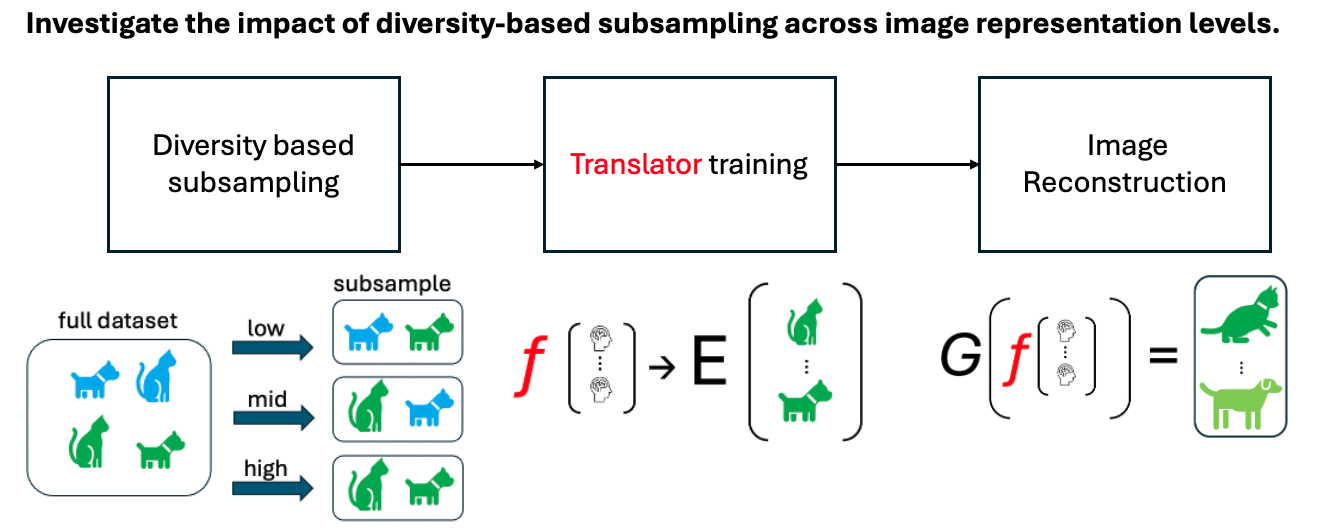
\includegraphics[width=1\textwidth]{plots/pipeline_exp1.png}
  \caption[Experiment 1: Pipeline]{Pipeline used in the first experiment. The goal of the experiment is written above. The subsampling process for three different feature spaces is depicted in the left diagram. The translators newly trained in this experiment are highlighted in red text. The translator is the function `$f$', the feature encoder (either VDVAE, CLIP or VGG19) is the function `E' and the image generator (either iCNN or versatile diffusion) is the function `G'}\label{fig:dropout_pipeline}
\end{figure}


\subsubsection{Baseline with random dropout}

\rTwo{In order to evaluate the diversity-based methods, it is important to establish a suitable baseline against which the results can be compared. To this end, reconstruction will first performed on a randomly subsampled training set. To get a better idea of the size of the training set needed to train the \rOne{translators}, different data fractions will be used. The full training set consists of 1200 images (and the corresponding recorded MRI activity). For the baseline, 10\% (120 images), 25\% (300 images), 50\% (600 images), 75\% (900 images) and 100\% of the images will first be used to train the \rOne{translator}. This baseline investigation will only be performed for one subject (S2) to save computational resources. To control the sampling error, 5 random samples will be taken for each data fraction and used to train the \rOne{translators}. If all training images are used, only one sample can be taken (the full data set). The results of this random baseline investigation will then be used to determine the sample size needed for the diversity based dropout.}


\subsubsection{Diversity based data subsampling}

For this work, the data should be subsampled as diversely as possible in order to produce a reduced dataset that can beat a randomly subsampled dataset in terms of \rOne{translation} and reconstruction performance. In this work, a multi-step subsampling procedure is chosen: First, all training images are transformed into a latent feature space. Within this feature space, an attempt is made to maximise diversity. Then, the nonlinear dimension reduction algorithm UMAP~\cite{mcinnesUMAPUniformManifold2018} is used to reduce the dimensionality of the training images' embeddedings in the respective feature space to two dimensions. The data in the UMAP space is then divided into $k$ clusters using k-means clustering (where $k$ is the number of images to be subsampled). For each of the $k$ clusters, the centroid of all $n$ images in that cluster is determined. Finally, for each cluster, the image with the smallest Euclidean distance to the centroid is selected. Using this procedure, $k$ images can be subsampled, where $k$ is arbitrary but must be less than the total number of training images. However, it should be clear that $k$ clusters cannot reasonably be found in the selected feature space; for example, if $k$ is selected very high (about 50\% of the dataset), only 2 images would be present in each cluster. To ensure that the subsampling algorithm can produce a meaningful subselection of the training set, k should be chosen as small as possible. Given the results of the random subselection baseline in the previous chapter, $k$ is set to 25\% (i.e. 300) of the images in the training set. 

% 4 UMAP
% plot in low_level_clustering.py
\begin{figure}[ht]
    \centering
    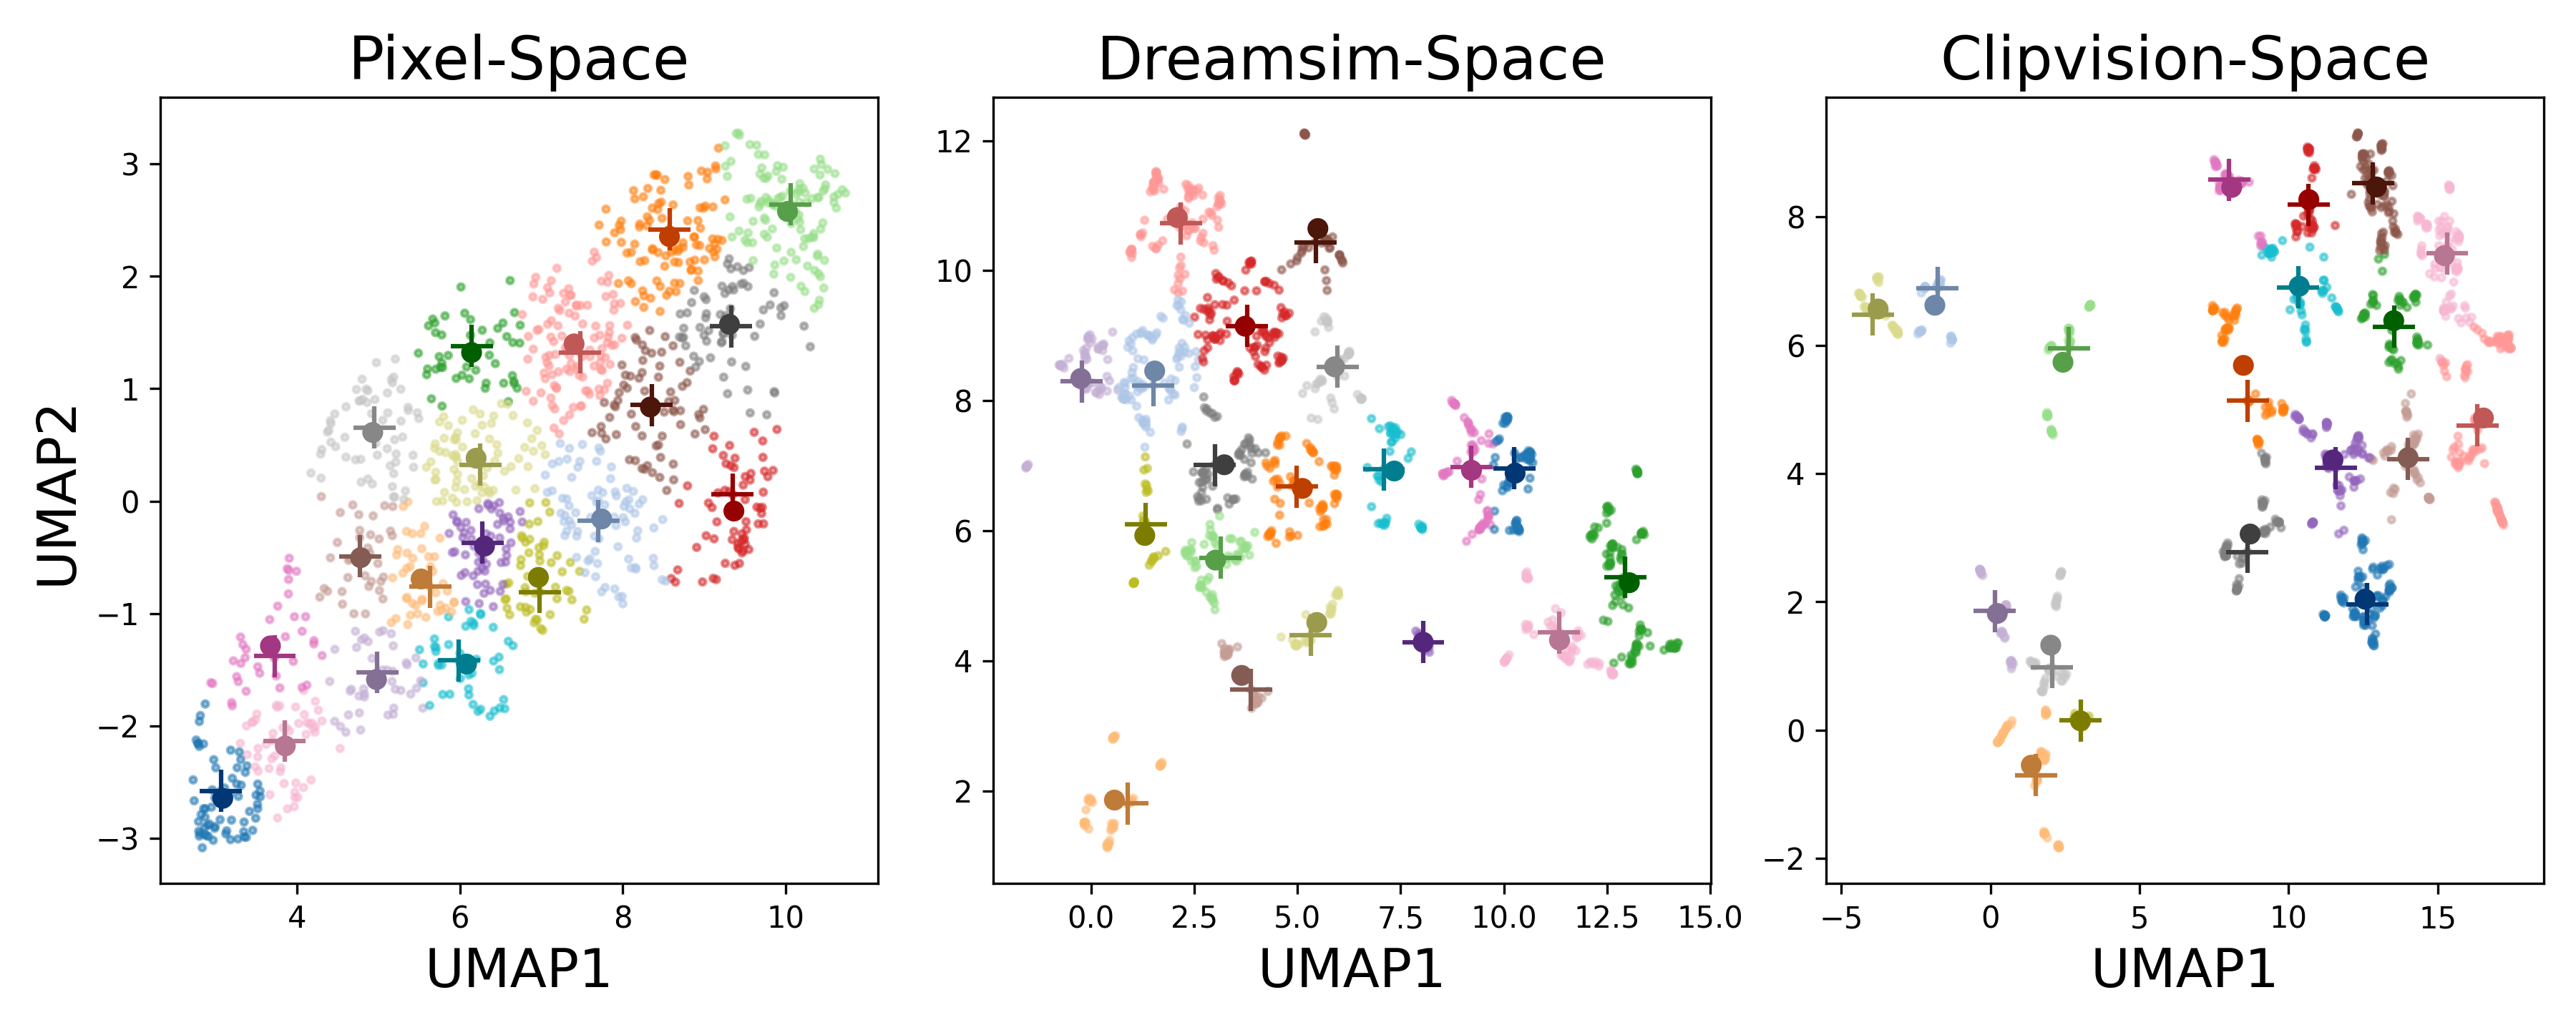
\includegraphics[width=0.9\textwidth]{plots/dropout_umap.png}
    \caption[UMAP visualization of diversity based subsampling]{Visualization of the two dimensional UMAP embeddings of the Pixel-Space, the DreamSim-space and the CLIP Vision space. Each point stands for one image in the training dataset. The x and y axis depict the dimensions that the UMAP algorithm computes. The points are colorized using k-means clustering (each cluster gets a different color). The mean value of all images in a cluster is visualized with a cross and the image that is closest to this mean value is visualized as a thick circle.}\label{fig:dropout_umap}
\end{figure}


The feature space in which the training images are initially embedded is freely selectable. To follow the logic of the evaluation criteria, a low-level, a mid-level and a high-level representation are chosen. For the low-level representation, the images (resized to 200$\times$200 pixels) are simply concatenated into a one-dimensional vector, so that the subsequent UMAP algorithm reduces the dimensions at the pixel level (this procedure was successfully applied by the authors of UMAP to the MNIST dataset). For the mid-level representation, the training images are embedded with DreamSim~\cite{fuDreamSimLearningNew2023}, for the high-level representation, the training images are embedded in CLIP-space using CLIP Vision~\cite{radfordLearningTransferableVisual2021}. Thus, all images are transformed into one-dimensional vectors whose dimensionality is reduced subsequently using UMAP and is then clustered using k-means. 
An example of the results of the selection process is shown in Figure~\ref{fig:dropout_umap}. In the plots, the number of clusters has been set to $k=20$ for visualisation purposes. Each point in the plot represents a sample of the training data set in UMAP space. Each cluster is coloured differently. The centroid of each cluster is shown as a circle and the image closest to the centroid is marked with a cross. In DreamSim and CLIP Vision space, the different clusters are already clearly separated from each other in the two dimensions of UMAP, while the result in pixel space has divided the images comparatively homogeneously, which may indicate that the UMAP dimension reduction has not worked optimally (this can probably be explained by the high number of dimensions in pixel space 200$\times$200$\times$3 colour channels = 120000). 

In order to ensure that the created subselection indeed increases the diversity in the feature space, it is validated quantitatively. For this purpose, a new metric is defined, the average minimum distance to all training samples (Average Min Distance). It is defined as follows:

\[
\text{Average Min Distance}
\coloneq \frac{1}{n_{\text{all}}}
  \sum_{i=1}^{n_{\text{all}}}
    \min_{1 \le j \le n_{\text{sub}}}
      \Bigl\lVert f(z_i) - f(z_j) \Bigr\rVert
\]

\noindent{}\rTwo{where \( n_{\text{all}} \) represents the number of images in the full dataset, \( n_{\text{sub}} \) represents the number of images in the subsample, \( z_i \) represents the $i$-th image in the full dataset, \( z_j \) represents the $j$-th image in the subsample, \( f \) represents embedding function from image to feature space and \( \|\cdot\| \) represents the Euclidean (L2) norm.}

The Average Min Distance measures how close on average each image in the full training dataset (embedded in the respective feature space) is to the closest image in the subsample. If the subsample adequately represents the feature space, then for each input image there would be a comparatively close candidate in the subsample. 

\subsection{Results}

\rTwo{The results of the random subsampling will be analyzed to determine a proper sample size for the diversity based dropout. Then the created diversity based subsamples will be analyzed. Finally, the the three diversity based subssamples and the random subsample will used to train the \rOne{translator} and reconstruct images for each of the five subjects.}


\subsubsection{Random dropout}

\begin{figure}[ht]
  \centering
  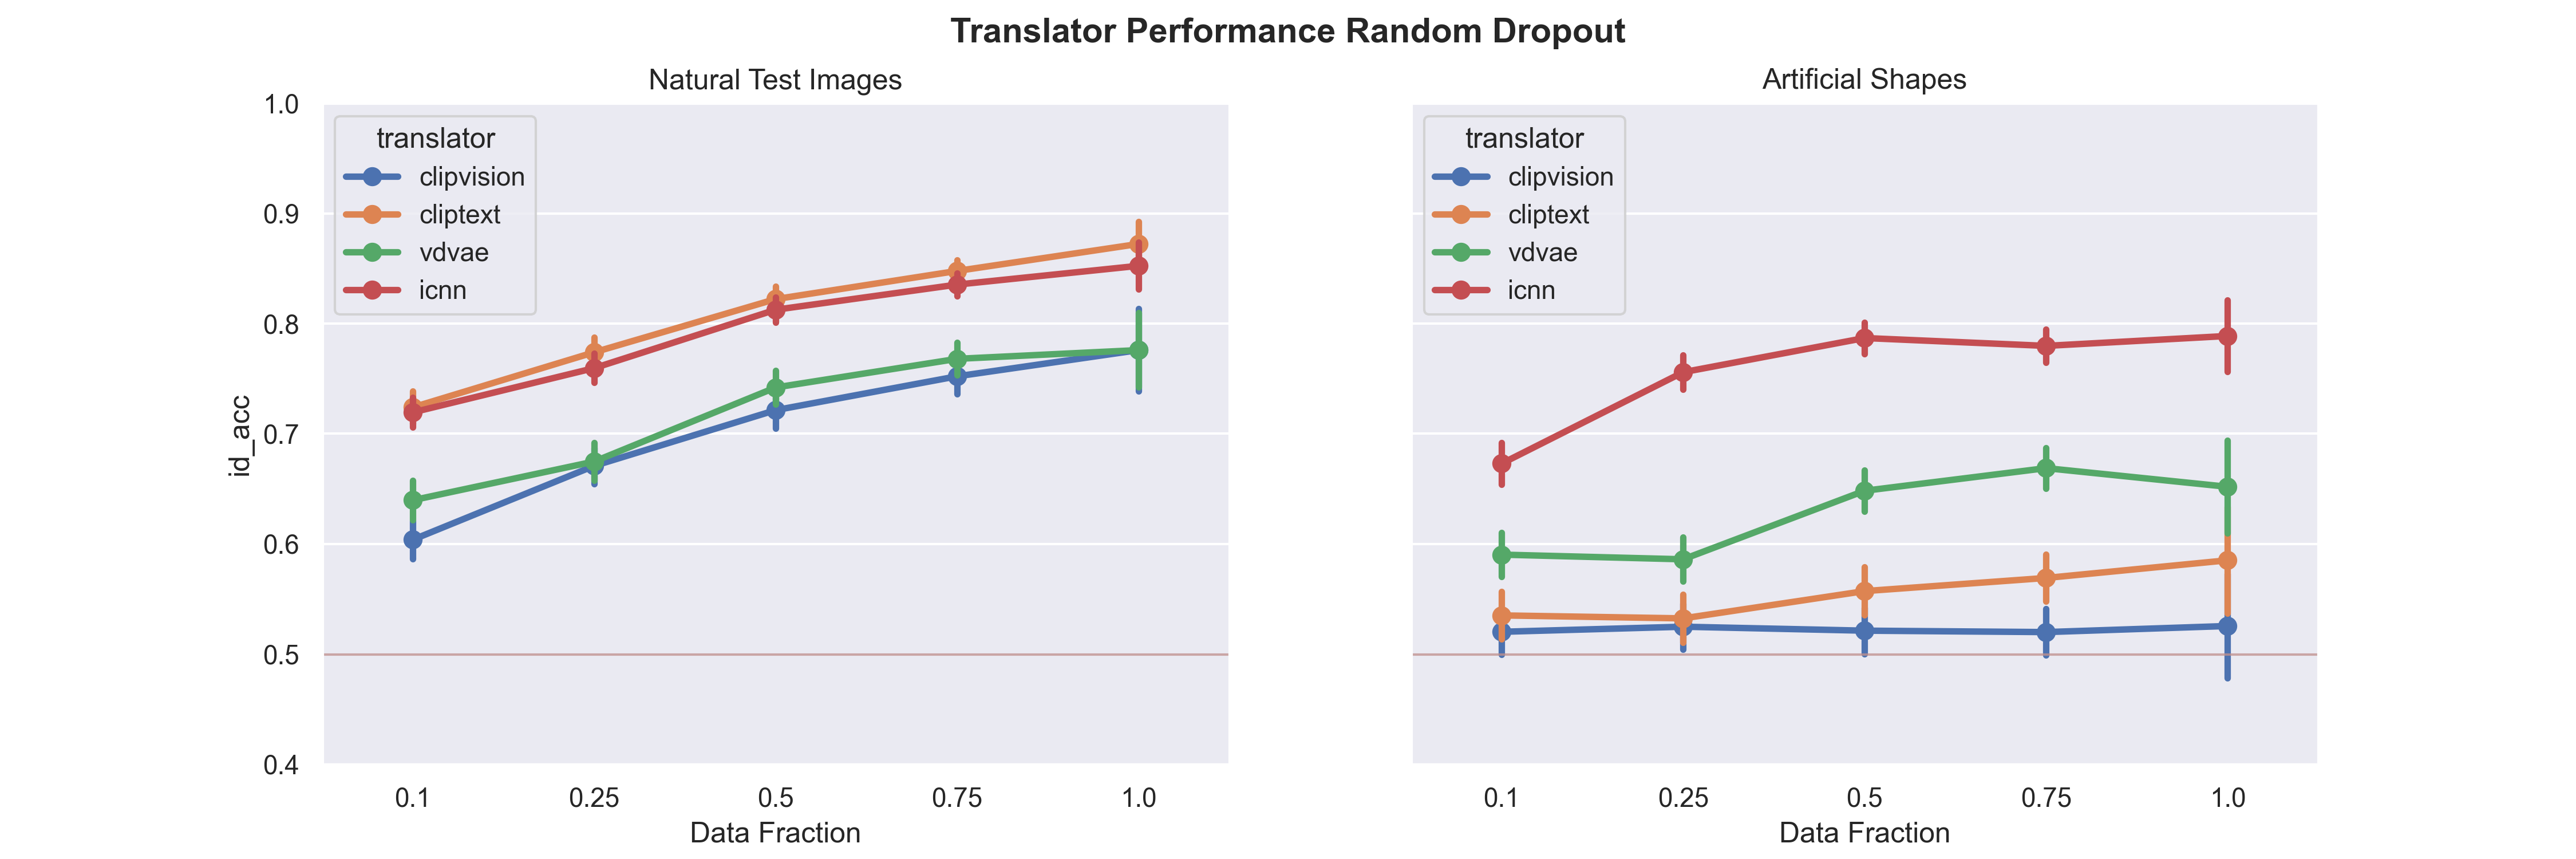
\includegraphics[width=1\textwidth]{plots/dropout_random_translator.png}
  \caption[Translator Performance with increasing dropout]{\rOne{Translator} Performance with different levels of random dropout \rOne{for subject S2. The four different translators were trained with random samples of the training dataset at different sizes (from 10\% to 75\% of the original size) and the performance is displayed using the identification accuracy. For each subsampled size, five random samples were drawn, the errorbars are computed as the standard error across the five subsamples.}}\label{fig:dropout_random_translator}
\end{figure}

The performance of the \rOne{translator} is shown in Figure~\ref{fig:dropout_random_translator} for both the natural test images and the artificial shapes. For the natural test images, the relationship between the number of training samples and performance is relatively similar for all the \rOne{translators}: the more training samples, the better. However, for the VDVAE and iCNN in particular, the performance curve for the \rOne{translator} flattens out at around 50\% training samples. The trend for the artificial shapes is somewhat different. The CLIP Vision \rOne{translator} does not seem to improve with an increasing number of training images, but is only just above the random level of 0.5. The \rTwo{CLIP Text} \rOne{translator} can show a performance above the random level from about 50\% of the training data set and then increases continuously. The VDVAE \rOne{translator} shows a slightly higher performance, but also saturates at about 50\% of the training data set. The same pattern is shown by the iCNN, whose performance is the best, but also does not improve after about 50\% of the training data set. 


\begin{figure}[ht]
  \centering
  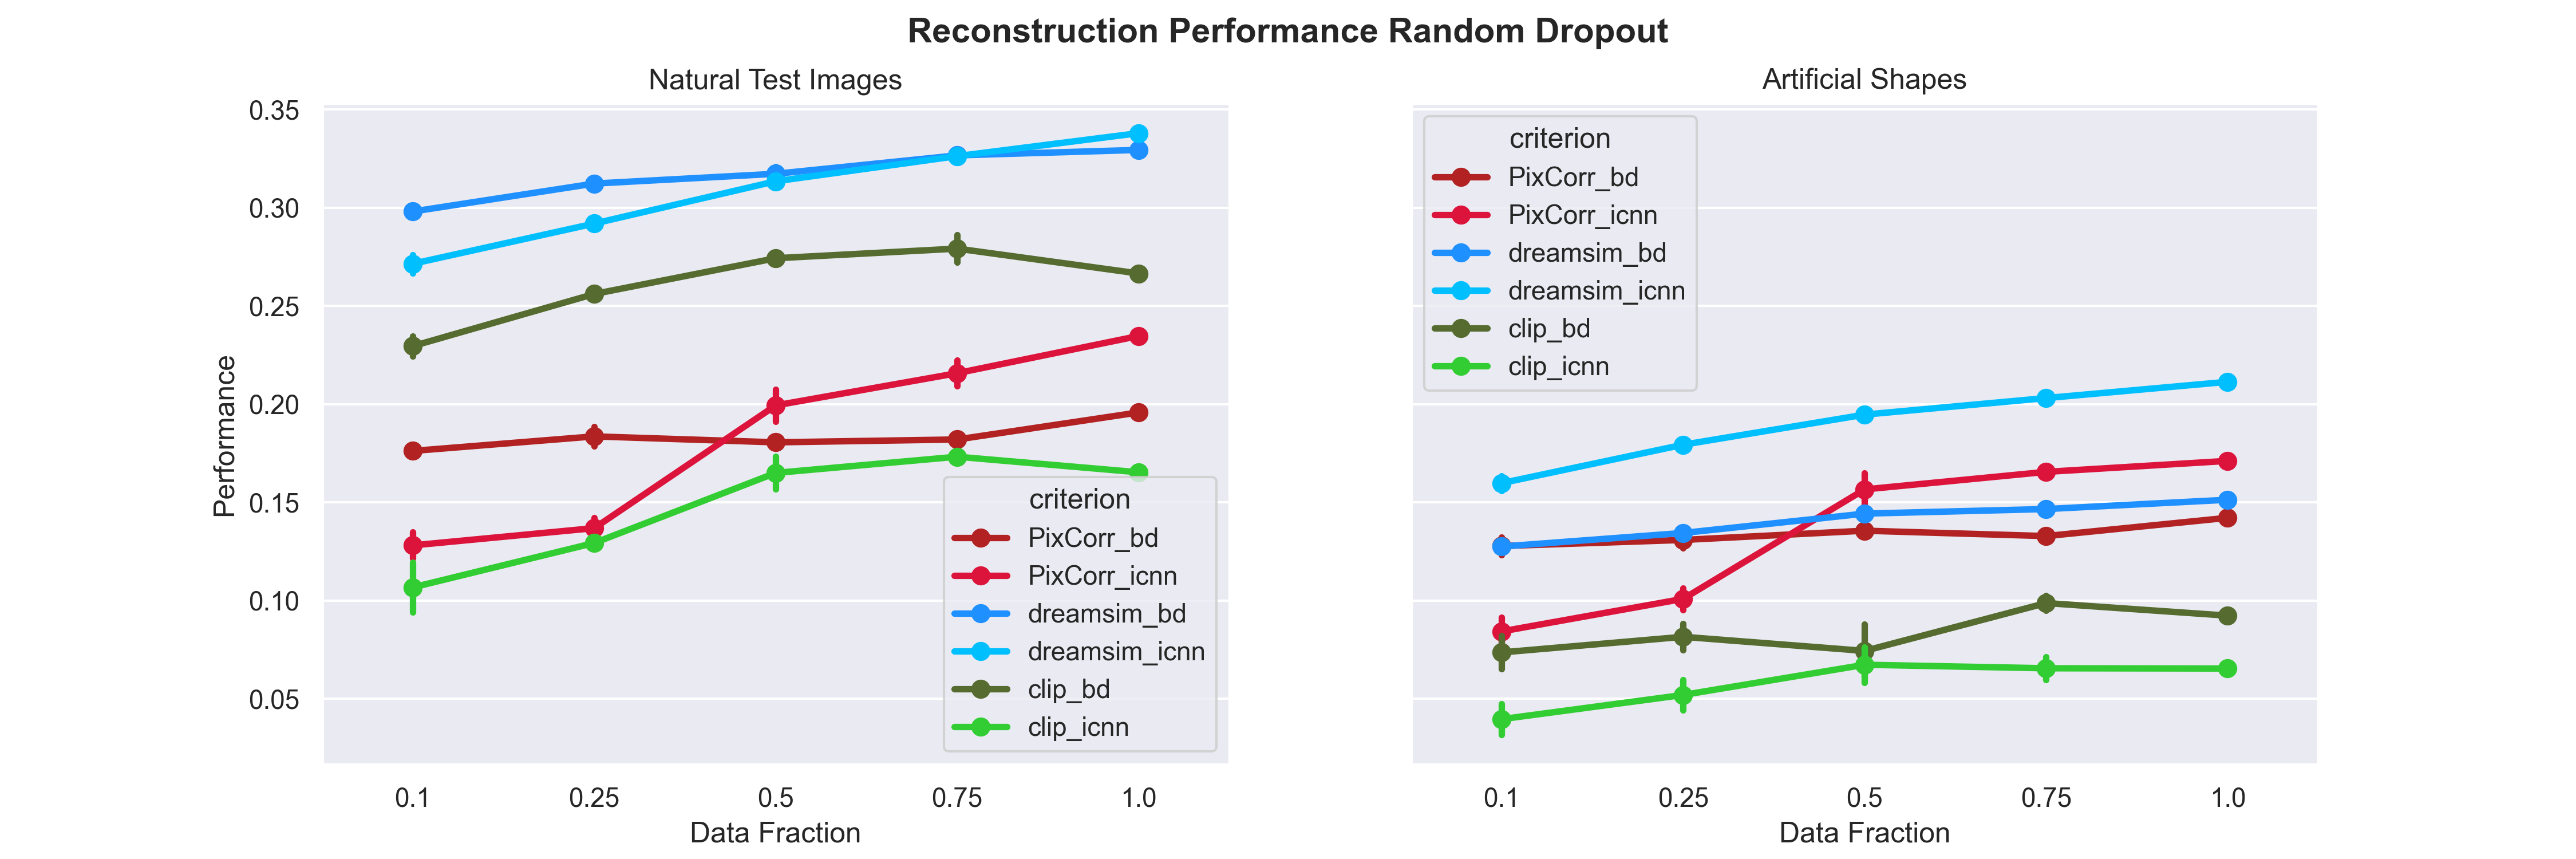
\includegraphics[width=1\textwidth]{plots/dropout_random_reconstruction.png}
  \caption[Reconstruction Performance with increasing dropout]{Reconstruction performance with different levels of random dropout for subject S2. The translators for the reconstruction algorithms were trained with random samples of the training dataset at different sizes (from 10\% to 75\% of the original size). The performance is displayed using the three reconstruction criteria PixelCorrelation, DreamSim and CLIP-accuracy. For each subsampled size, five random samples were drawn, the errorbars are computed as the standard error across the five subsamples.}\label{fig:dropout_random_reconstruction}
\end{figure}

The quantitative performance of the reconstruction algorithms is shown in Figure~\ref{fig:dropout_random_reconstruction} for both the natural test images and the artificial images. The PixelCorrelation shows a similar picture for both algorithms for the natural test images and the artificial shapes: While the iCNN benefits from more training samples, with the step from 25\% to 50\% of the training data set being particularly significant, the Brain-Diffuser shows only a very small increase in performance with increasing number of training samples. The DreamSim similarity increases continuously with a larger number of training samples. In particular, the iCNN benefits from a larger number of training samples. The CLIP-accuracy shows that for the natural test images the performance also saturates at about 50\% of the training samples, the same goes for the artificial shapes.

\begin{figure}[]
  \centering
  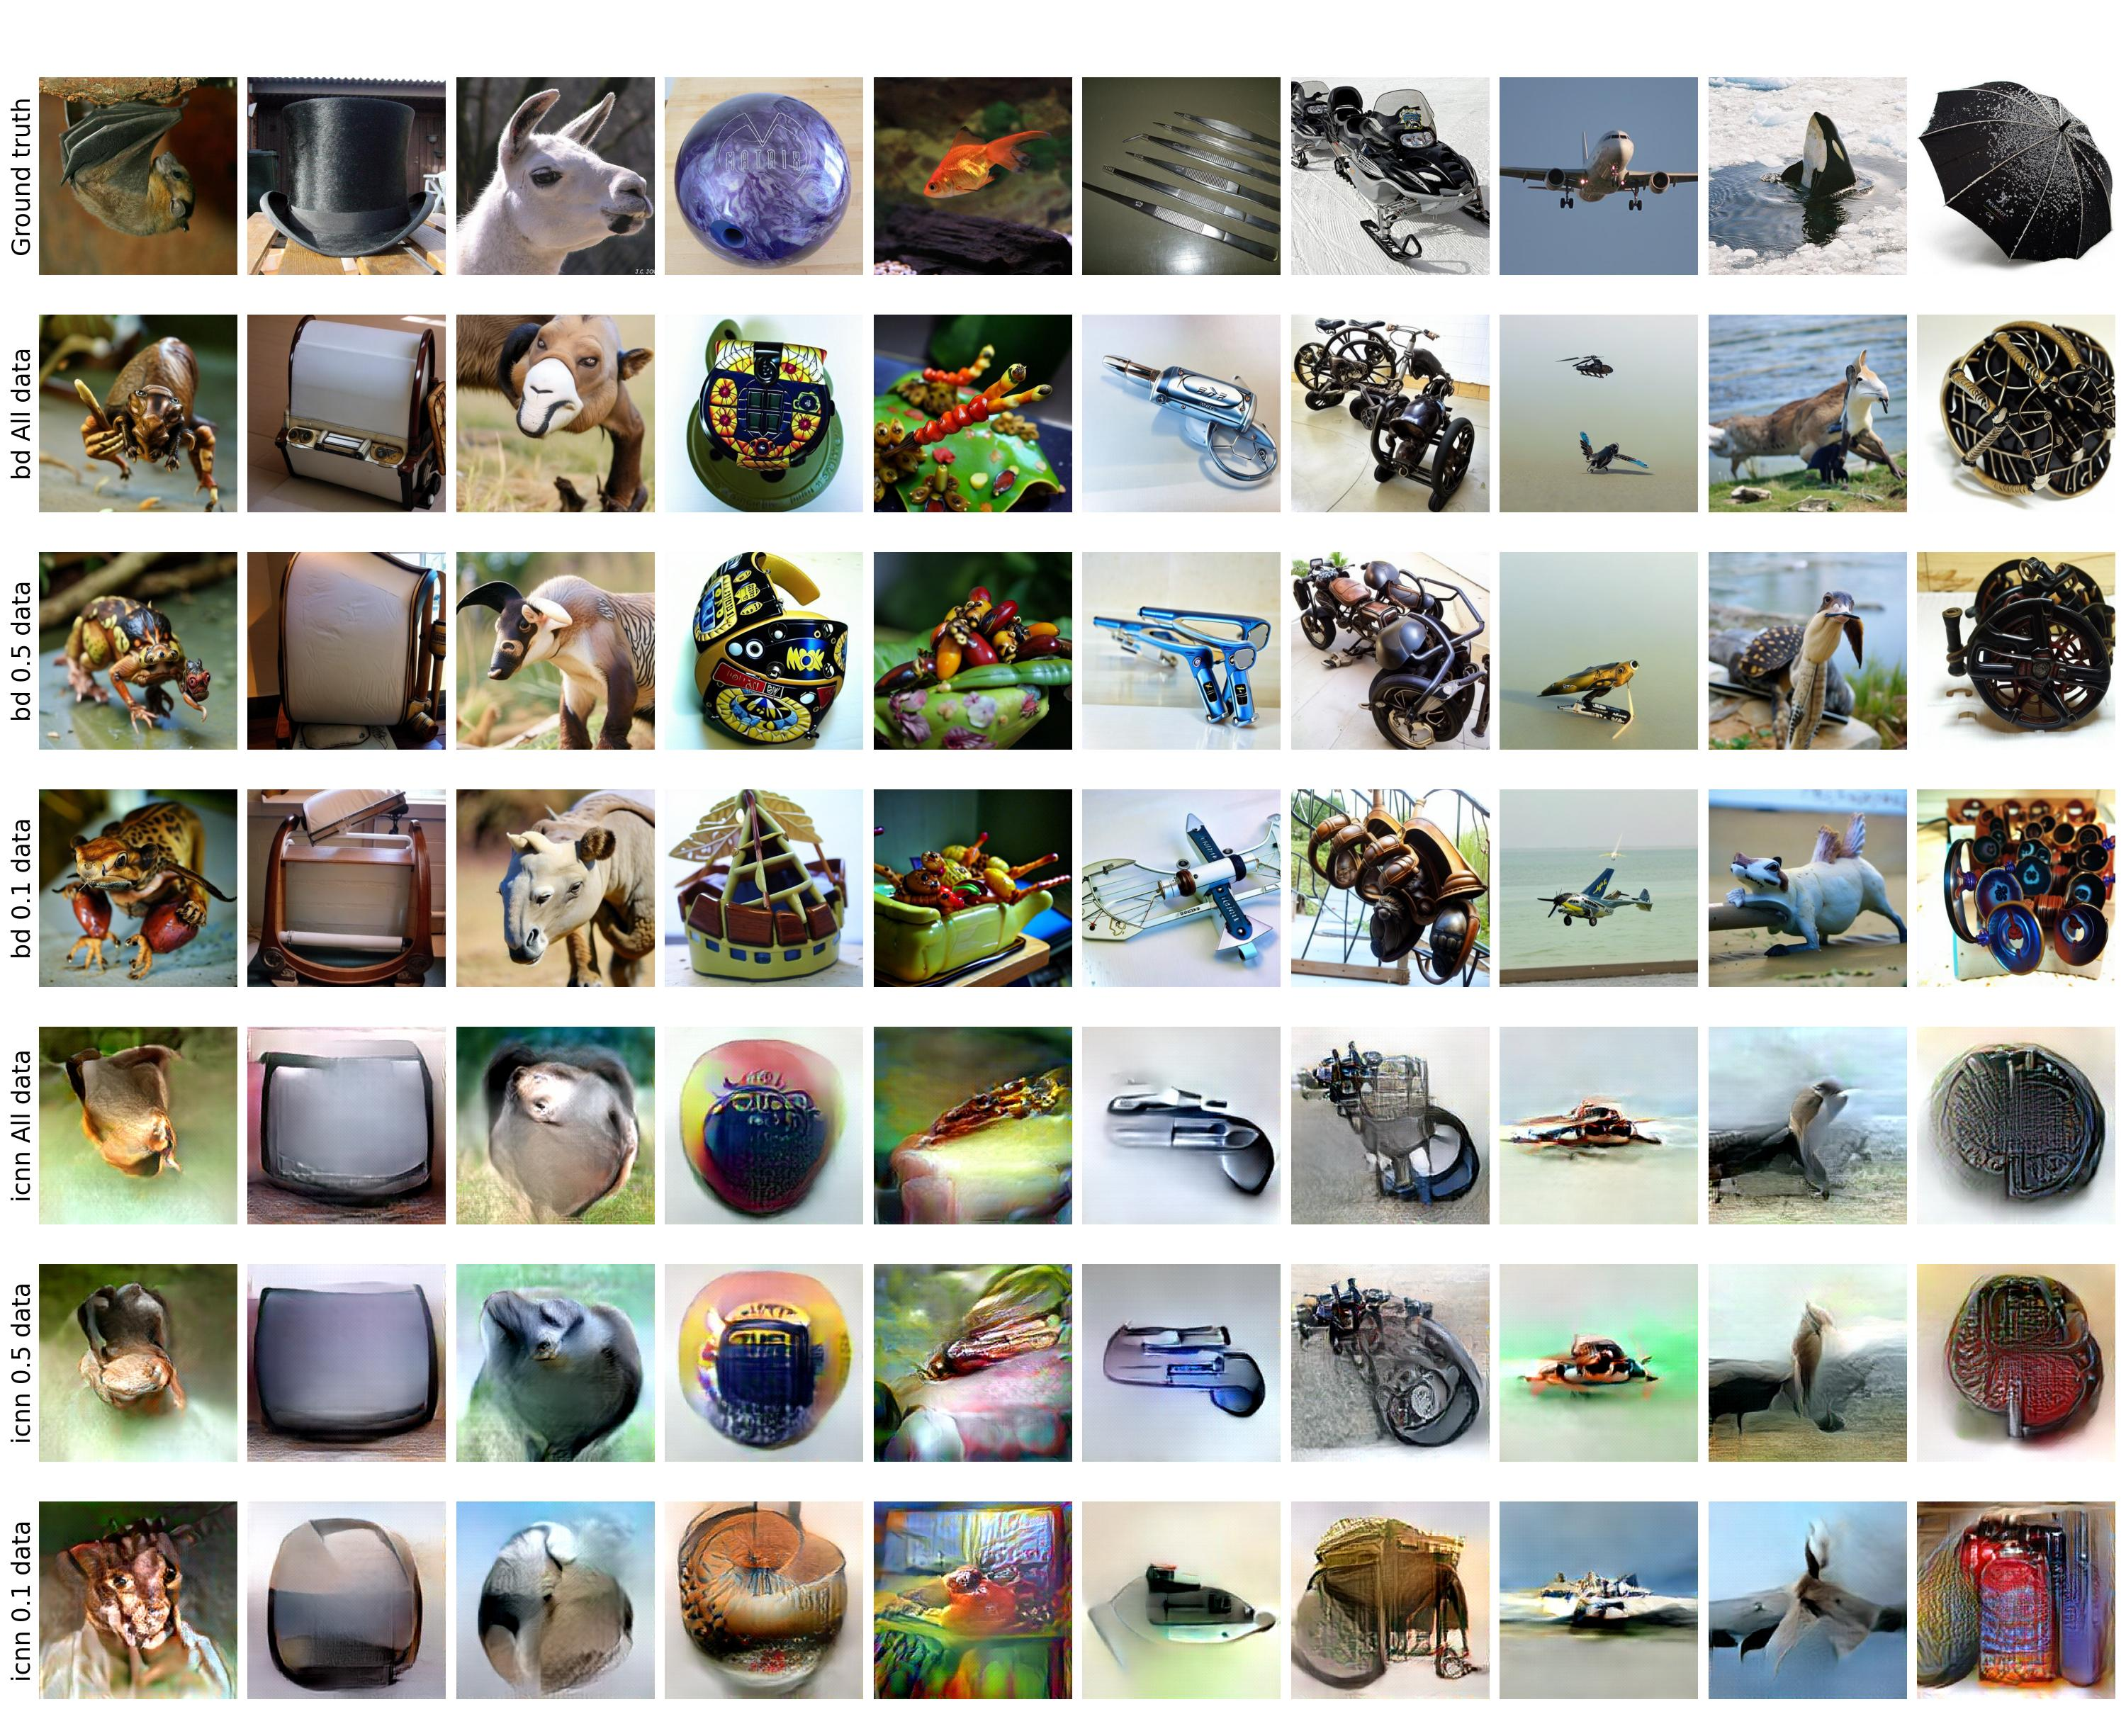
\includegraphics[width=1\textwidth]{plots/dropout_qual_random_test.JPEG}
  \caption[Qualitative results random dropout on natural test images]{Qualitative results with different levels of random dropout on natural test images. In the first row, the ground truth images are displayed. In the following three rows, the reconstructed images from the Brain-Diffuser are displayed with three different sizes of the training data (either all data, a 50\% random subsample of the data and a 10\% random subsample of the data). In the last three rows, the reconstruction results from the iCNN are displayed, again with the three different training dataset sizes.}\label{fig:dropout_qual_random_test}
\end{figure}


The qualitative performance of the reconstructions with different training set sizes can be seen in Figure~\ref{fig:dropout_qual_random_test} for the natural test images. It can be seen that even with only 10\% of the training images, distinctive features of the images can be reconstructed, \rTwo{while it is also visible, that} the quality of the reconstructions improves as the amount of training data increases. For example, the Brain-Diffuser is not yet able to correctly classify the snowmobile as a vehicle with a small amount of training data, or the outlines of the goldfish are not yet nearly correct with the iCNN.\@ Interestingly, the reconstruction of the Brain-Diffuser's aircraft is better with a small number of training samples than with the full data set. This is probably because the VDVAE, which produced artefacts for this image, still works with the small number of training samples. \rTwo{For the artificial shapes a very similar picture emerges, the quality of reconstructions improves visibly with an increased number of training samples. An example of their reconstruction for the random dropout can be seen in the appendix in Figure~\ref{fig:dropout_qual_random_art}.}


In summary, it can be said that the performance in \rOne{translation} and reconstruction can usually be significantly improved with an increasing number of training samples. In our example, many effects become visible in the step between 25\% and 50\% of the training data set, and in some cases the performance starts to saturate from this point on. For the following experiments, therefore, the data set should not contain more than 50\% of the training samples, in order to still have potential for performance improvement. At the same time, the training data set should not be smaller than 25\%, otherwise the \rOne{translation} may not work well enough for testing.


\subsubsection{Diversity based dropout}
\rTwo{According to the previously described procedure to gain diversity based subsamples,} subsamples with 25\% (300 images) of the training data set were extracted for each of the feature spaces using the method described above. Figure~\ref{fig:dropout_similarity_plot} shows an example of five training dataset images (left column), where the most similar image in the subsampled dataset in the respective feature space is displayed. This shows the differences in sampling in the three feature spaces: in the DreamSim and CLIP Vision spaces, the images are relatively similar to the original. \rTwo{There are small} differences between the mid-level and high-level similarities that become clear. For example, in the case of the revolver in the first image, DreamSim selects a gun that is relatively similar in the image, but is the wrong type. CLIP Vision selects an image that is a better semantic match because it also shows a revolver, even though the remaining visual similarity is lower (colour of the gun, partially covered by a hand). This difference between CLIP Vision and DreamSim can also be seen in other images. In pixel space the subjective similarity between the original and the sample is lower and based on the low-level features of the input images disregarding semantic similarities. In the third image, for example, the original shows an ear with white headphones, while the most similar image in pixel space is a goose with a long white neck. The low-level match between the images is presumably an elongated white object in the middle. 

% 5 Umap Subselection Similarity from low_level_clustering.py
% dropout similarity plot is in gimp I believe
\begin{figure}[ht]
  \centering
  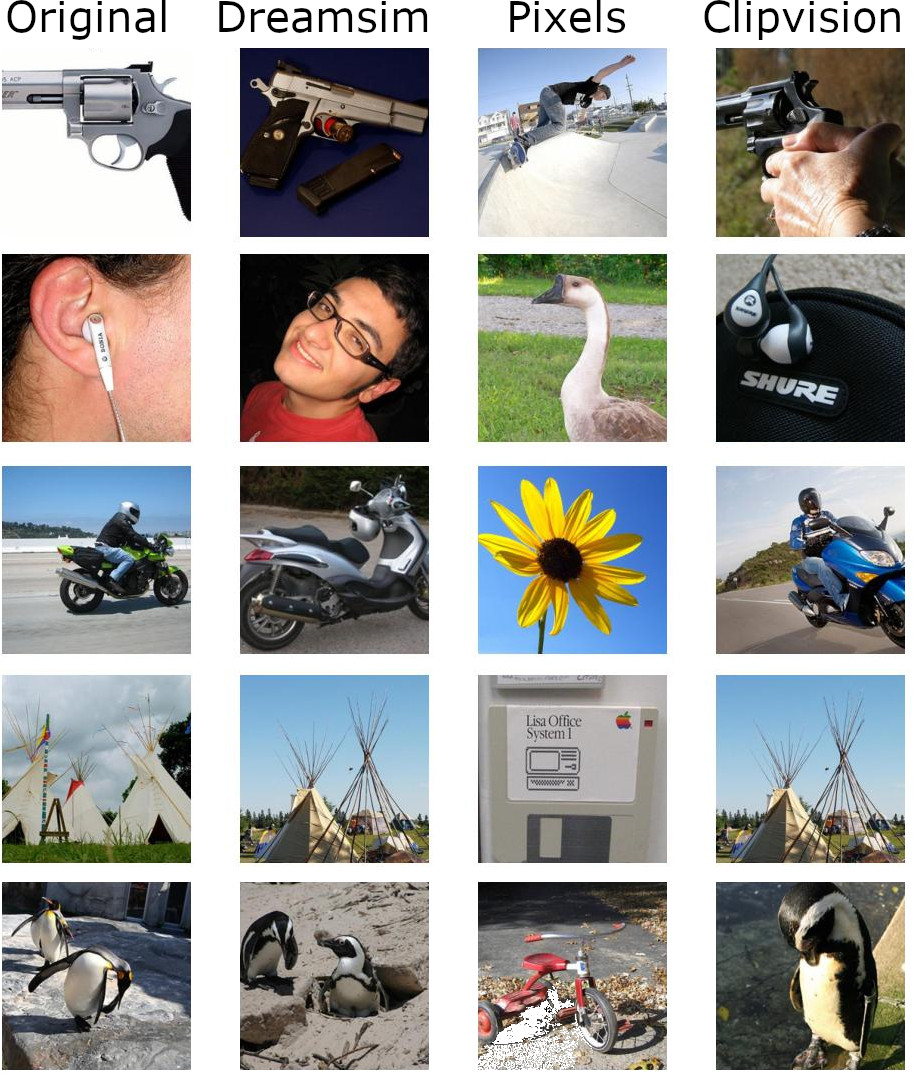
\includegraphics[width=0.5\textwidth]{plots/dropout_similarity_plot.JPEG}
  \caption[Qualitative results of diversity based subsampling]{Qualitative results of diversity based subsampling. In the left column, a random selection of 5 images from the original training dataset is shown. In the following columns, the most similar image to that original image in subsample based on the respective feature space (DreamSim, pixels and CLIP Vision) is shown.}\label{fig:dropout_similarity_plot}
\end{figure}

\rTwo{To measure if the subselections have properly increased the diversity in their respective subspaces, the previously described Average Min Distance is calculated for all three feature spaces }and is shown in Figure~\ref{fig:dropout_avg_min_distance}. For each subspace, 30 different samples were taken and the Average Min Distance was calculated for each sample. The figure shows that in each feature space, the subsample created using the corresponding feature space has the lowest Average Min Distance. The result is most ambiguous for the Average Min Distance in the pixel feature space, but again the subsample created using the pixel space has the lowest Average Min Distance. The Average Min Distance for DreamSim and CLIP Vision are always comparatively close, which makes sense since DreamSim is partly based on CLIP Vision~\cite{fuDreamSimLearningNew2023}. In summary, the qualitative and quantitative review showed that the diversity-based subsampling method is successful in increasing the diversity in the respective subspace. For each feature space, the subsample with the lowest Average Min Distance in the validation (i.e.\ best representing the entire feature space) is used for further analysis.

\begin{figure}[ht]
  \centering
  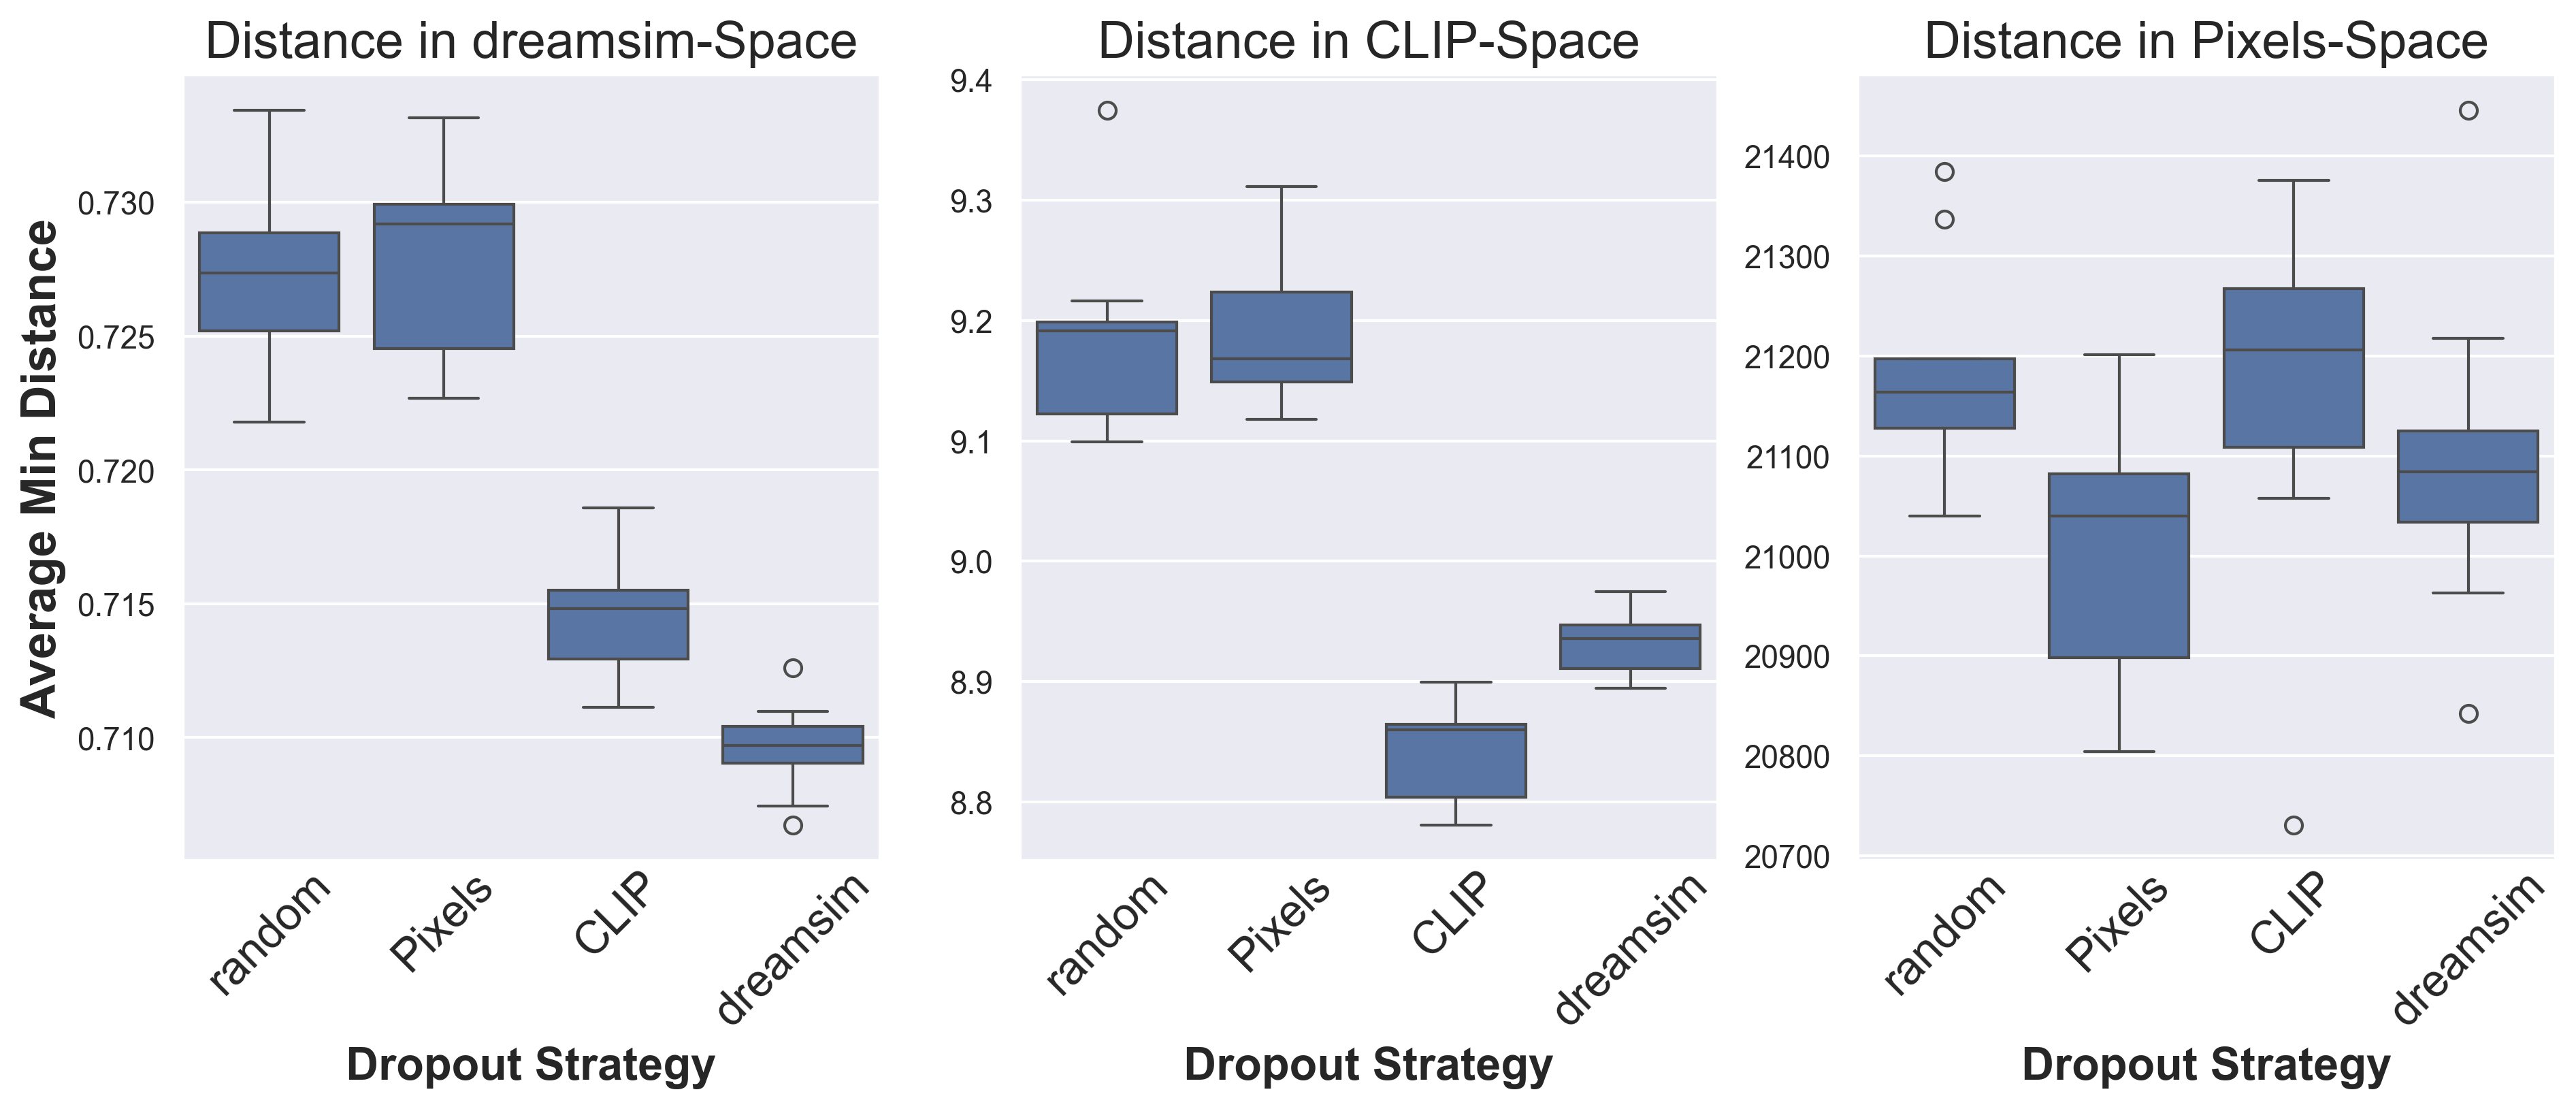
\includegraphics[width=1\textwidth]{plots/dropout_avg_min_distance.png}
  \caption[Average Min Distance with different dropout strategies]{Average Min Distance of multiple drawn subsamples. For each of the four dropout strategies (random and the three different features spaces), 30 samples with 25\% of the original dataset size were drawn. The Average Min Distance was computed within the three feature spaces and its distribution across the 30 samples is plotted.}\label{fig:dropout_avg_min_distance}
\end{figure}


\subsubsection{Translator performance}
The performance of the three trained \rOne{translators} of the Brain-Diffuser and the iCNN algorithm is shown in Figure~\ref{fig:dropout_eval_translator_test} for the natural test images. The results are shown for all four different dropout strategies (random subsample and samples based on the three feature spaces). The performance of all subsamples is above the random probability of 0.5. However, for the three \rOne{translators} of the Brain-Diffuser, there are no discernible differences in performance between the different dropout strategies. Only the iCNN \rOne{translator} shows that performance can be slightly improved with a targeted diversity-based subsampling strategy. \rTwo{In} this case too, there is no significant difference between the three feature spaces. The artificial shapes in Figure~\ref{fig:dropout_eval_translator_art} show that the two CLIP translators are not able to predict the features significantly beyond random probability. This is independent of the subsampling space. The performance of the VDVAE translator is slightly better, with all subsamples tending to have a higher performance than the random probability. In particular, the performance of the low-level pixel feature space seems to have a slight advantage over the other subsampling strategies. For the iCNN translator, on the other hand, the effect of the natural test images seems to have been reversed; for the Pixel and DreamSim feature spaces, the performance even looks slightly worse than with random subsampling. Within the CLIP Vision feature space, the variance between the subjects is really high, thus the results cannot easily be interpreted.

% Now the Eval Results
% 7.1 Eval decoder test
\begin{figure}[ht]
  \centering
  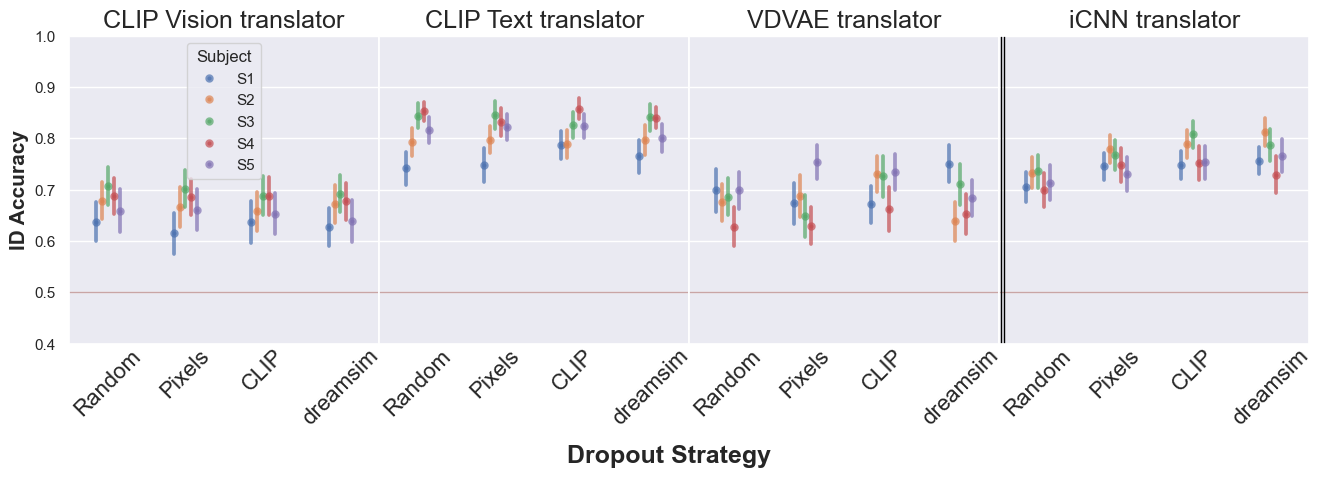
\includegraphics[width=1\textwidth]{plots/dropout_eval_translator_test.png}
  \caption[Experiment 1: Translator performance for natural test images]{\rOne{Translator} performance (0.25 data fraction) for natural test images. The identification accuracy for all four translators (three from Brain-Diffuser and one from iCNN) are displayed for the subsamples computed with the four dropout strategies. The data is shown for each subject and the error bars are computed as the standard errors across all test samples.}\label{fig:dropout_eval_translator_test}
\end{figure}


\begin{figure}[ht]
  \centering
  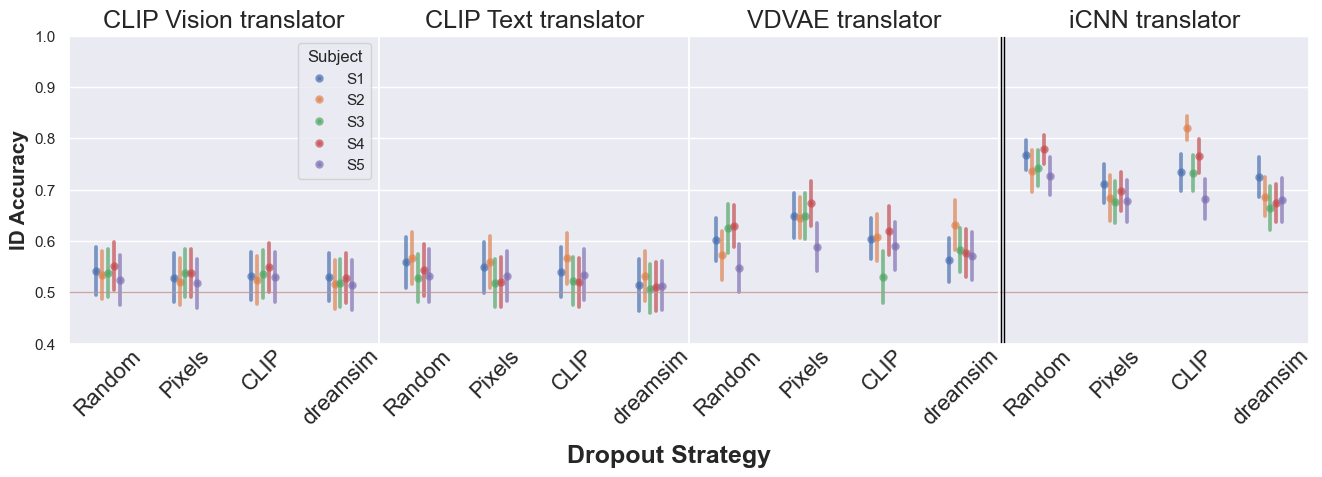
\includegraphics[width=1\textwidth]{plots/dropout_eval_translator_art.png}
  \caption[Experiment 1: Translator performance for artificial shapes]{\rOne{Translator} performance (0.25 data fraction) for artificial shapes. The identification accuracy for all four translators (three from Brain-Diffuser and one from iCNN) are displayed for the subsamples computed with the four dropout strategies. The data is shown for each subject and the error bars are computed as the standard errors across all test samples.}\label{fig:dropout_eval_translator_art}
\end{figure}


\subsubsection{Reconstruction performance}

\begin{figure}[ht]
  \centering
  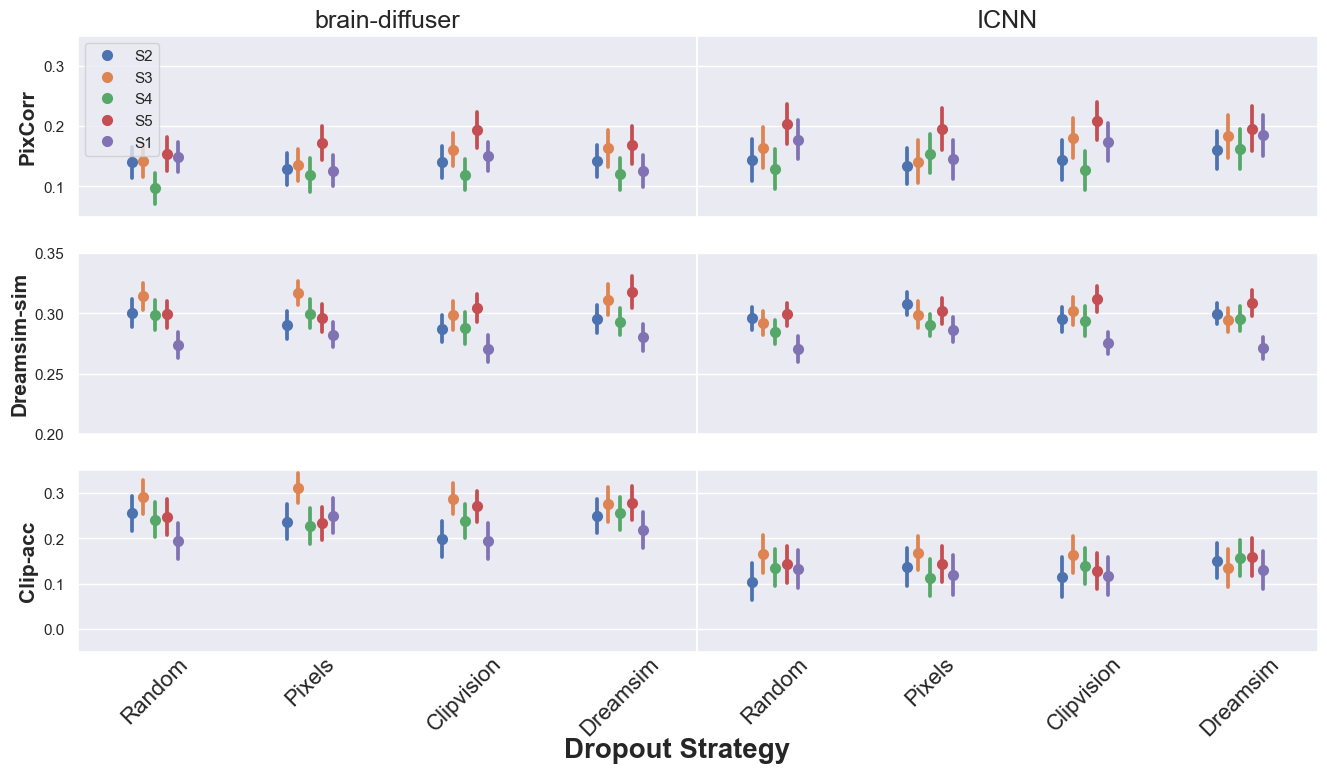
\includegraphics[width=1\textwidth]{plots/dropout_eval_reconstruction_test.png}
  \caption[Experiment 1: Reconstruction performance for natural test images]{Reconstruction Performance (0.25 data fraction) for natural test images. For each of the five subjects, the three reconstruction criteria (PixelCorrelation, DreamSim and CLIP-accuracy) are displayed for both the Brain-Diffuser and iCNN algorithm using the subsamples computed with the four dropout strategies. The errorbars are computed as the standard error across all the test samples.}\label{fig:dropout_eval_reconstruction_test}
\end{figure}

The quantitative results of the reconstructions using the four different subsamples are shown in Figure~\ref{fig:dropout_eval_reconstruction_test} for the natural test images. The three previously described criteria of PixelCorrelation, DreamSim-similarity and CLIP-accuracy are displayed for the Brain-Diffuser and iCNN algorithms respectively. There is no discernible difference between the random subselection and the three diversity-based subsamples for the Brain-Diffuser in any of the three metrics. The results are similar for the iCNN.\@ Although the translator performance was improved beforehand, these effects seem to have only a minor impact on the reconstruction performance. Only with the help of the DreamSim-similarity metric is there a slight increase in performance across all three feature spaces in contrast to the random baseline. There are again no differences between the feature spaces. Also for the artificial shapes in Figure~\ref{fig:dropout_eval_reconstruction_art}, the differences in reconstruction performance between the different feature spaces are small. For the Brain-Diffuser it looks as if the pixel correlation with a dropout is slightly increased in the pixel subspace compared to the baseline. \rThree{However measured with the DreamSim and CLIP-accuracy, it looks like the diversity based subsampling performs even worse than the random subsampling.} In the iCNN, the DreamSim similarity appears slightly reduced in Pixels subspace and CLIP Vision subspace compared to the baseline. There are no visible differences in the DreamSim subspace.

\begin{figure}[ht]
  \centering
  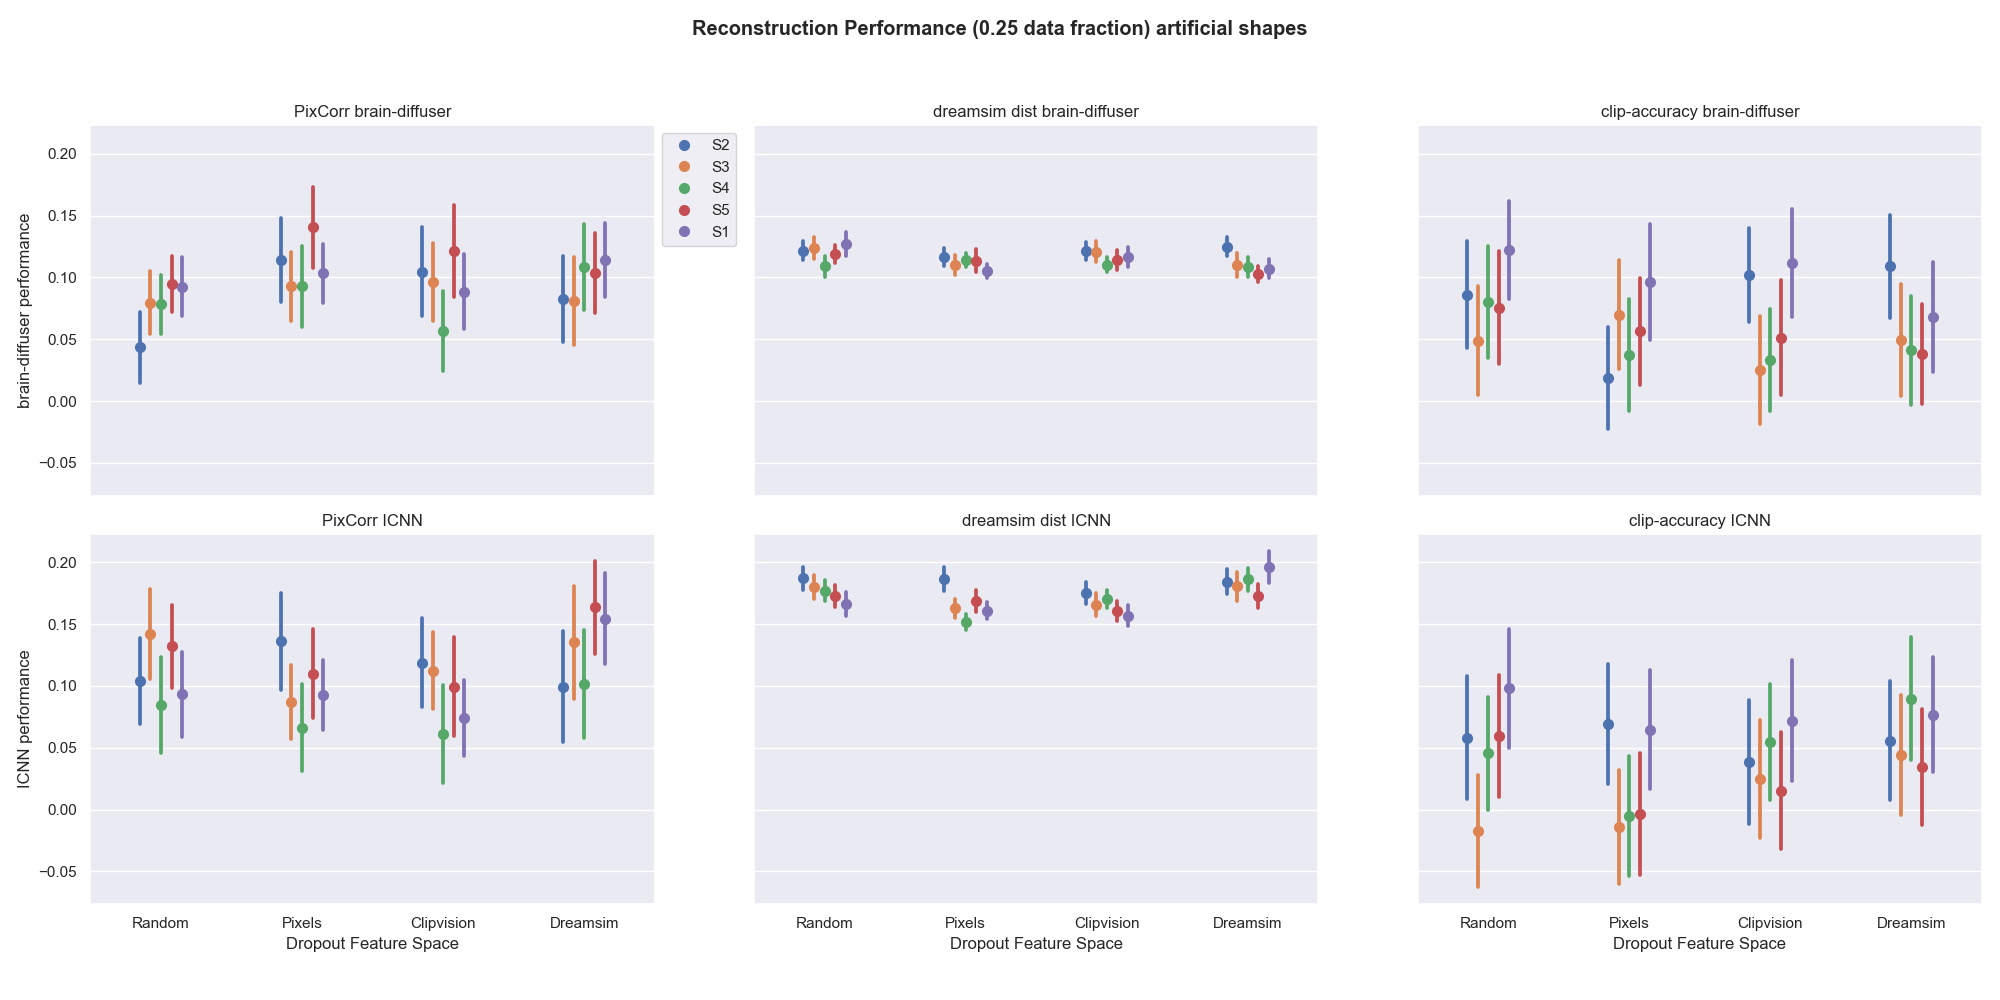
\includegraphics[width=1\textwidth]{plots/dropout_eval_reconstruction_art.png}
  \caption[Experiment 1: Reconstruction performance for artificial shapes]{Reconstruction Performance (0.25 data fraction) for artificial shapes. For each of the five subjects, the three reconstruction criteria (PixelCorrelation, DreamSim and CLIP-accuracy) are displayed for both the Brain-Diffuser and iCNN algorithm using the subsamples computed with the four dropout strategies. The errorbars are computed as the standard error across all the test samples.}\label{fig:dropout_eval_reconstruction_art}
\end{figure}


\begin{figure}[ht]
  \centering
  \includegraphics[width=1\textwidth]{plots/dropout_qual_eval_icnn_test.JPEG}
  \caption[Experiment 1: Reconstructed images for iCNN on natural test images]{Qualitative results for different dropout strategies with the iCNN on natural test images. The top row depicts the ground truth image. Each following row depicts the reconstruction where the translator was trained using the dropout strategy defined on the left side.}\label{fig:dropout_qual_eval_icnn_test}
\end{figure}

As the quantitative results of the reconstruction performance suggest, a qualitative assessment of the differences in the reconstruction is difficult. The iCNN results for the natural test images are shown in Figure~\ref{fig:dropout_qual_eval_icnn_test}. Differences in the quality of the reconstruction are difficult to determine; although it is clear that at least some reconstruction quality can be achieved in all conditions, the slight improvement of the feature spaces in contrast to the random baseline  seen in the quantitative results is not immediately apparent in the actual images. Likewise, for the artificial shapes in Figure~\ref{fig:dropout_qual_eval_icnn_art}, the slight degradation in the feature space results compared to the random sample is not directly apparent from the qualitative results. The quantitative results for the Brain-Diffuser were even more ambiguous, so no major differences can be seen in the qualitative analysis of the images. The reconstructed images for the Brain-Diffuser can be found in the appendix (Figure~\ref{fig:dropout_qual_eval_bd_test} for the natural test images and Figure~\ref{fig:dropout_qual_eval_bd_art} for the artificial shapes).


\begin{figure}[ht]
  \centering
  \includegraphics[width=1\textwidth]{plots/dropout_qual_eval_icnn_art.JPEG}
  \caption[Experiment 1: Reconstructed images for iCNN on artificial shapes]{Qualitative results for different dropout strategies with the iCNN on artificial shapes. The top row depicts the ground truth image. Each following row depicts the reconstruction where the translator was trained using the dropout strategy defined on the left side.}\label{fig:dropout_qual_eval_icnn_art}
\end{figure}

\subsection{Discussion}
  
\rTwo{Our initial hypotheses were only partially confirmed, revealing more complex relationships between data diversity and reconstruction performance than anticipated. We hypothesized that low-level feature diversity improves performance on artificial shapes, high-level diversity benefits natural images, and mid-level diversity provides the best overall performance. The results revealed several unexpected patterns that provide new insights into how different aspects of visual information are processed and reconstructed from brain activity.} For the Brain-Diffuser, there were generally few differences between the different subsamples. Only for the artificial shapes could the translator performance and also the pixel correlation of the reconstruction be increased by low-level subsampling. This is consistent with the hypothesis that low-level subsampling improves low-level reconstruction. However, as this effect can only be measured with the pixel correlation, it should be treated with caution and could only have occurred by chance. \rThree{The subsampling in the other two subspaces however seems to have slightly worsened the reconstructions of artificial shapes}. With the iCNN the results were somewhat clearer. In the case of the natural test images, the \rOne{translator} could be improved by any type of subsampling, and the subsequent reconstructions could also be improved (measured with DreamSim). Interestingly, this effect is exactly the opposite for the artificial shapes. Here, diversity-based subsampling even seems to be disadvantageous compared to random subsampling: both the \rOne{translator} and the reconstruction performance decrease compared to the baseline. 

\subsubsection{Exploring the influence of monotone training data}
In the following, we will further investigate why the performance of the artificial shapes is presumably reduced by diversity-based subsampling. A closer look at the training images reveals that there are some images that show individual central objects with a monotonous (usually white) background. It could be that these are similar in concept to the artificial shapes. In this sense, the artificial shapes are not really out-of-distribution samples, because a monotone background of the training images is not really natural either. It is investigated whether these images have a significant influence on the reconstruction. In order to test this, a new, reduced training data set is created, which mainly contains these images. A simple algorithm is used to identify these images in the training dataset automatically: The colour values for each pixel in all images are counted, and then the images are sorted according to how often the most frequent pixel occurs in each image (so an image with a white background would have the colour white as most frequent color, which occurs extremely often). In Figure~\ref{fig:dropout_discussion_monohetero_qual}, the 5 most monotonous images found by the algorithm (i.e.\ those where the most frequent colour occurs very often) are compared with the 5 most heterogeneous images (i.e.\ those where the colours are more evenly distributed). As can be seen, the subdivision of the images using this algorithm worked well. In the following, \rOne{translators} consisting of 0.25 (i.e. 300 images) of the training data for the most homogeneous and heterogeneous as defined by the algorithm explained above set are trained again.


\begin{figure}[ht]
  \centering
  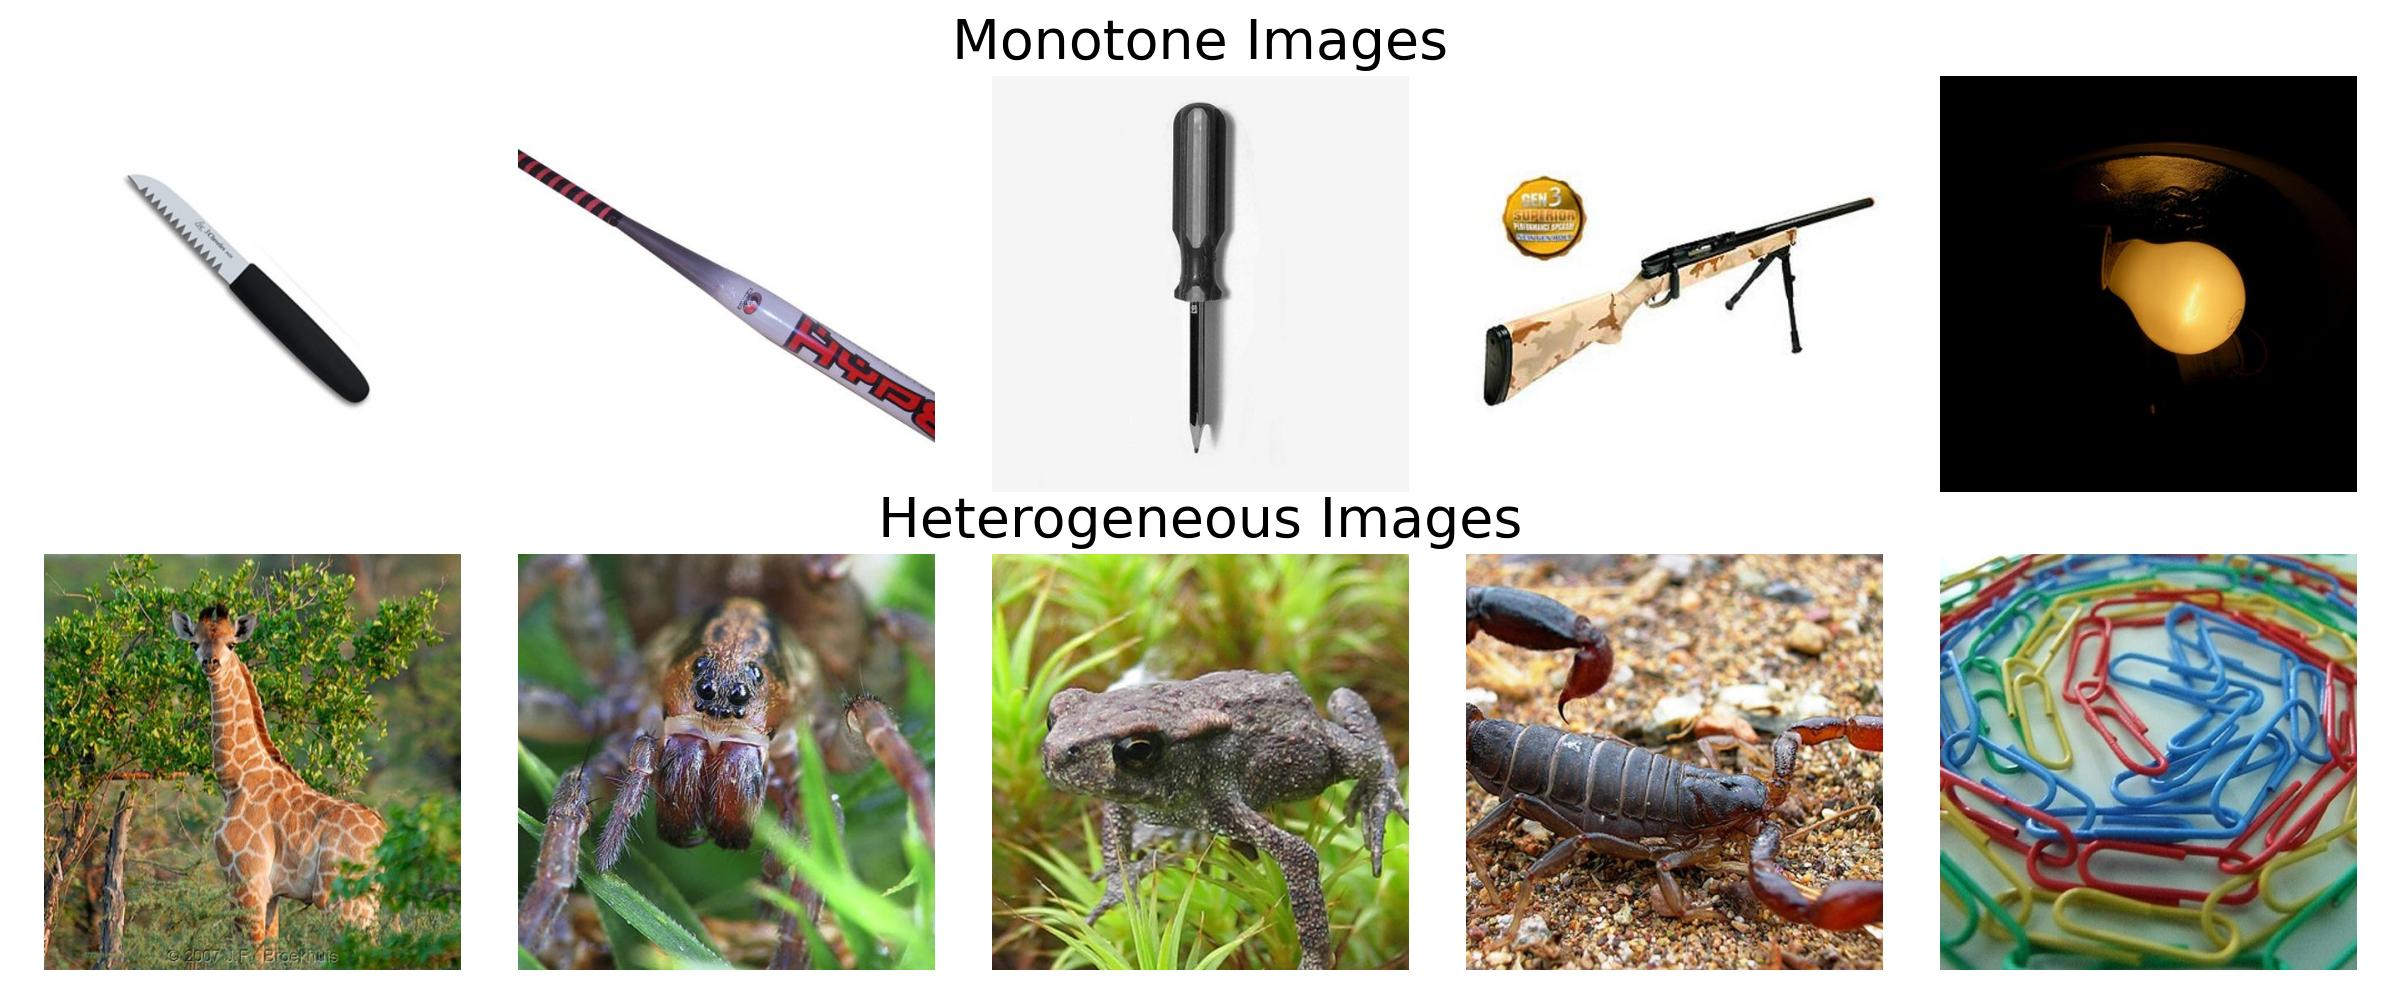
\includegraphics[width=0.75\textwidth]{plots/dropout_discussion_monohetero_qual.jpeg}
  \caption[Monotone and heterogeneous samples in the training dataset]{Comparison of monotone and heterogeneous training images (the five most monotone and heterogeneous samples are displayed).}\label{fig:dropout_discussion_monohetero_qual}
\end{figure}

% \begin{figure}[ht]
%   \centering
%   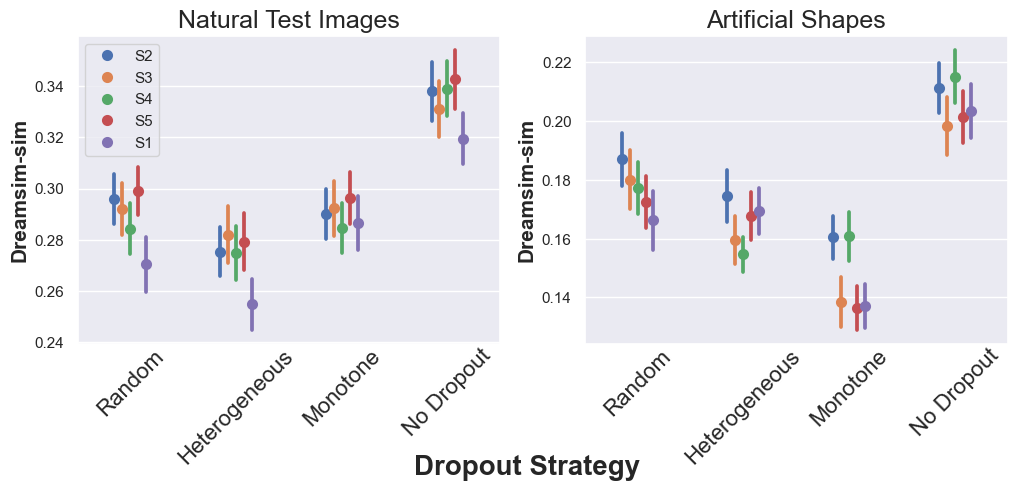
\includegraphics[width=1\textwidth]{plots/dropout_discussion_reconstruction_icnn.png}
%   \caption[iCNN reconstruction performance monotone vs.\ heterogeneous training sample]{iCNN reconstruction results for monotone vs.\ heterogeneous training images. The DreamSim reconstruction metric is displayed for all five participants depending on the dropout strategy. The results for both the natural test images and artificial chapes are displayed. The error bars are computed as the standard error across all test samples.}\label{fig:dropout_discussion_reconstruction_icnn}
% \end{figure}

The quantitative results of the reconstructions with the monotonous and heterogeneous subsample training datasets are shown in Figure~\ref{fig:dropout_discussion_reconstruction} for both the natural test images and the artificial shapes. \rThree{For the iCNN}, the random dropout performs better than both monotonous and heterogeneous subsampling. Contrary to expectation, monotonous subsampling actually performs worse than heterogeneous subsampling with artificial shapes. \rTwo{The} results for the Brain-Diffuser are quite different. As expected, random subsampling performs best for natural test images. For the artificial shapes, however, there is a clear effect: monotonous subsampling leads to significantly increased performance than heterogeneous subsampling. It is even on par with the performance that can be expected, if there is no dropout at all (all training images are used). This effect is also best illustrated by the qualitative reconstructions for the natural test images in Figure~\ref{fig:dropout_discussion_test} (the qualitative results for the artificial shapes are shown in Figure~\ref{fig:dropout_discussion_art} in the appendix): for each image reconstructed with the Brain-Diffuser, a monochrome background can be seen in the monotonous condition. In contrast, all backgrounds show multiple details when the heterogeneous training data is used. This also shows why the results of the iCNN for the artificial shapes are not necessarily improved by using monotonous training: the reconstructions with the iCNN have a comparatively neutral background when both monotonous and heterogeneous training data are used. All results for the four different translators for monotonous vs.\ heterogeneous training data are shown in the appendix in figures~\ref{fig:dropout_discussion_translator_id_acc_cliptext},~\ref{fig:dropout_discussion_translator_id_acc_clipvision},~\ref{fig:dropout_discussion_translator_id_acc_vdvae},~\ref{fig:dropout_discussion_translator_id_acc_icnn}. 

The insights that can be gained from this additional investigation using monotonous and heterogeneous training data subsets are twofold. On the one hand, the Brain-Diffuser can be strongly conditioned to reconstruct single objects with monotonous backgrounds, so that the performance for the artificial images can be greatly improved by the background of the images alone. There is even no quantitative performance increase if all training images would be used instead of only the ones with monotone background. On the other hand, it can be seen that the iCNN generally seems to produce images with neutral backgrounds and a central object in the middle (this can also be checked with the other qualitative results in this experiment). It therefore seems that the iCNN has a bias towards this type of image, where single central objects are displayed on a neutral background, regardless of the nature of the training data. The reason for this bias in the iCNN might be the pre-training of the model on the ImageNet~\cite{dengImageNetLargescaleHierarchical2009} dataset --- the images also mostly feature a prominent object in the middle. Another reason for this phenomenon could lie in the way the visual attention works. It has been shown that visual attention strongly modulates the translation of brain-activity~\cite{horikawaAttentionModulatesNeural2022}. Since the participants probably focused on the prominent central aspects of the images when their brain activity was recorded, only these central aspects of the training images might have caught the attention of the subjects, thus having a stronger representation in the brain activity~\cite{wolfeVisualAttention2000}. 


\begin{figure}[ht]
  \centering
  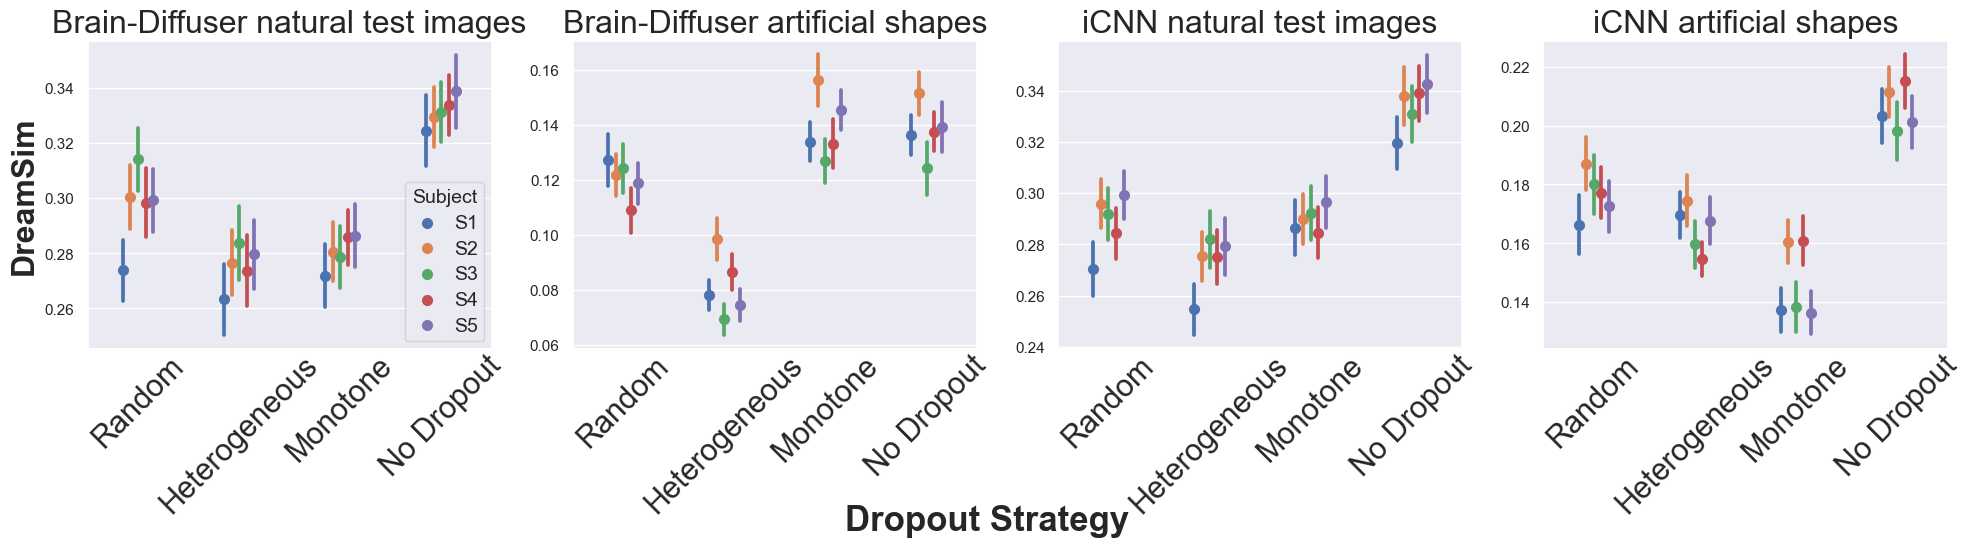
\includegraphics[width=1\textwidth]{plots/dropout_discussion_reconstruction.png}
  \caption[Reconstruction performance monotone vs.\ heterogeneous training sample]{Reconstruction results for monotone vs.\ heterogeneous training images. The DreamSim reconstruction metric is displayed for all five participants depending on the dropout strategy. The results for both the natural test images and artificial chapes are displayed. The error bars are computed as the standard error across all test samples.}\label{fig:dropout_discussion_reconstruction}
\end{figure}


\begin{figure}[ht]
  \centering
  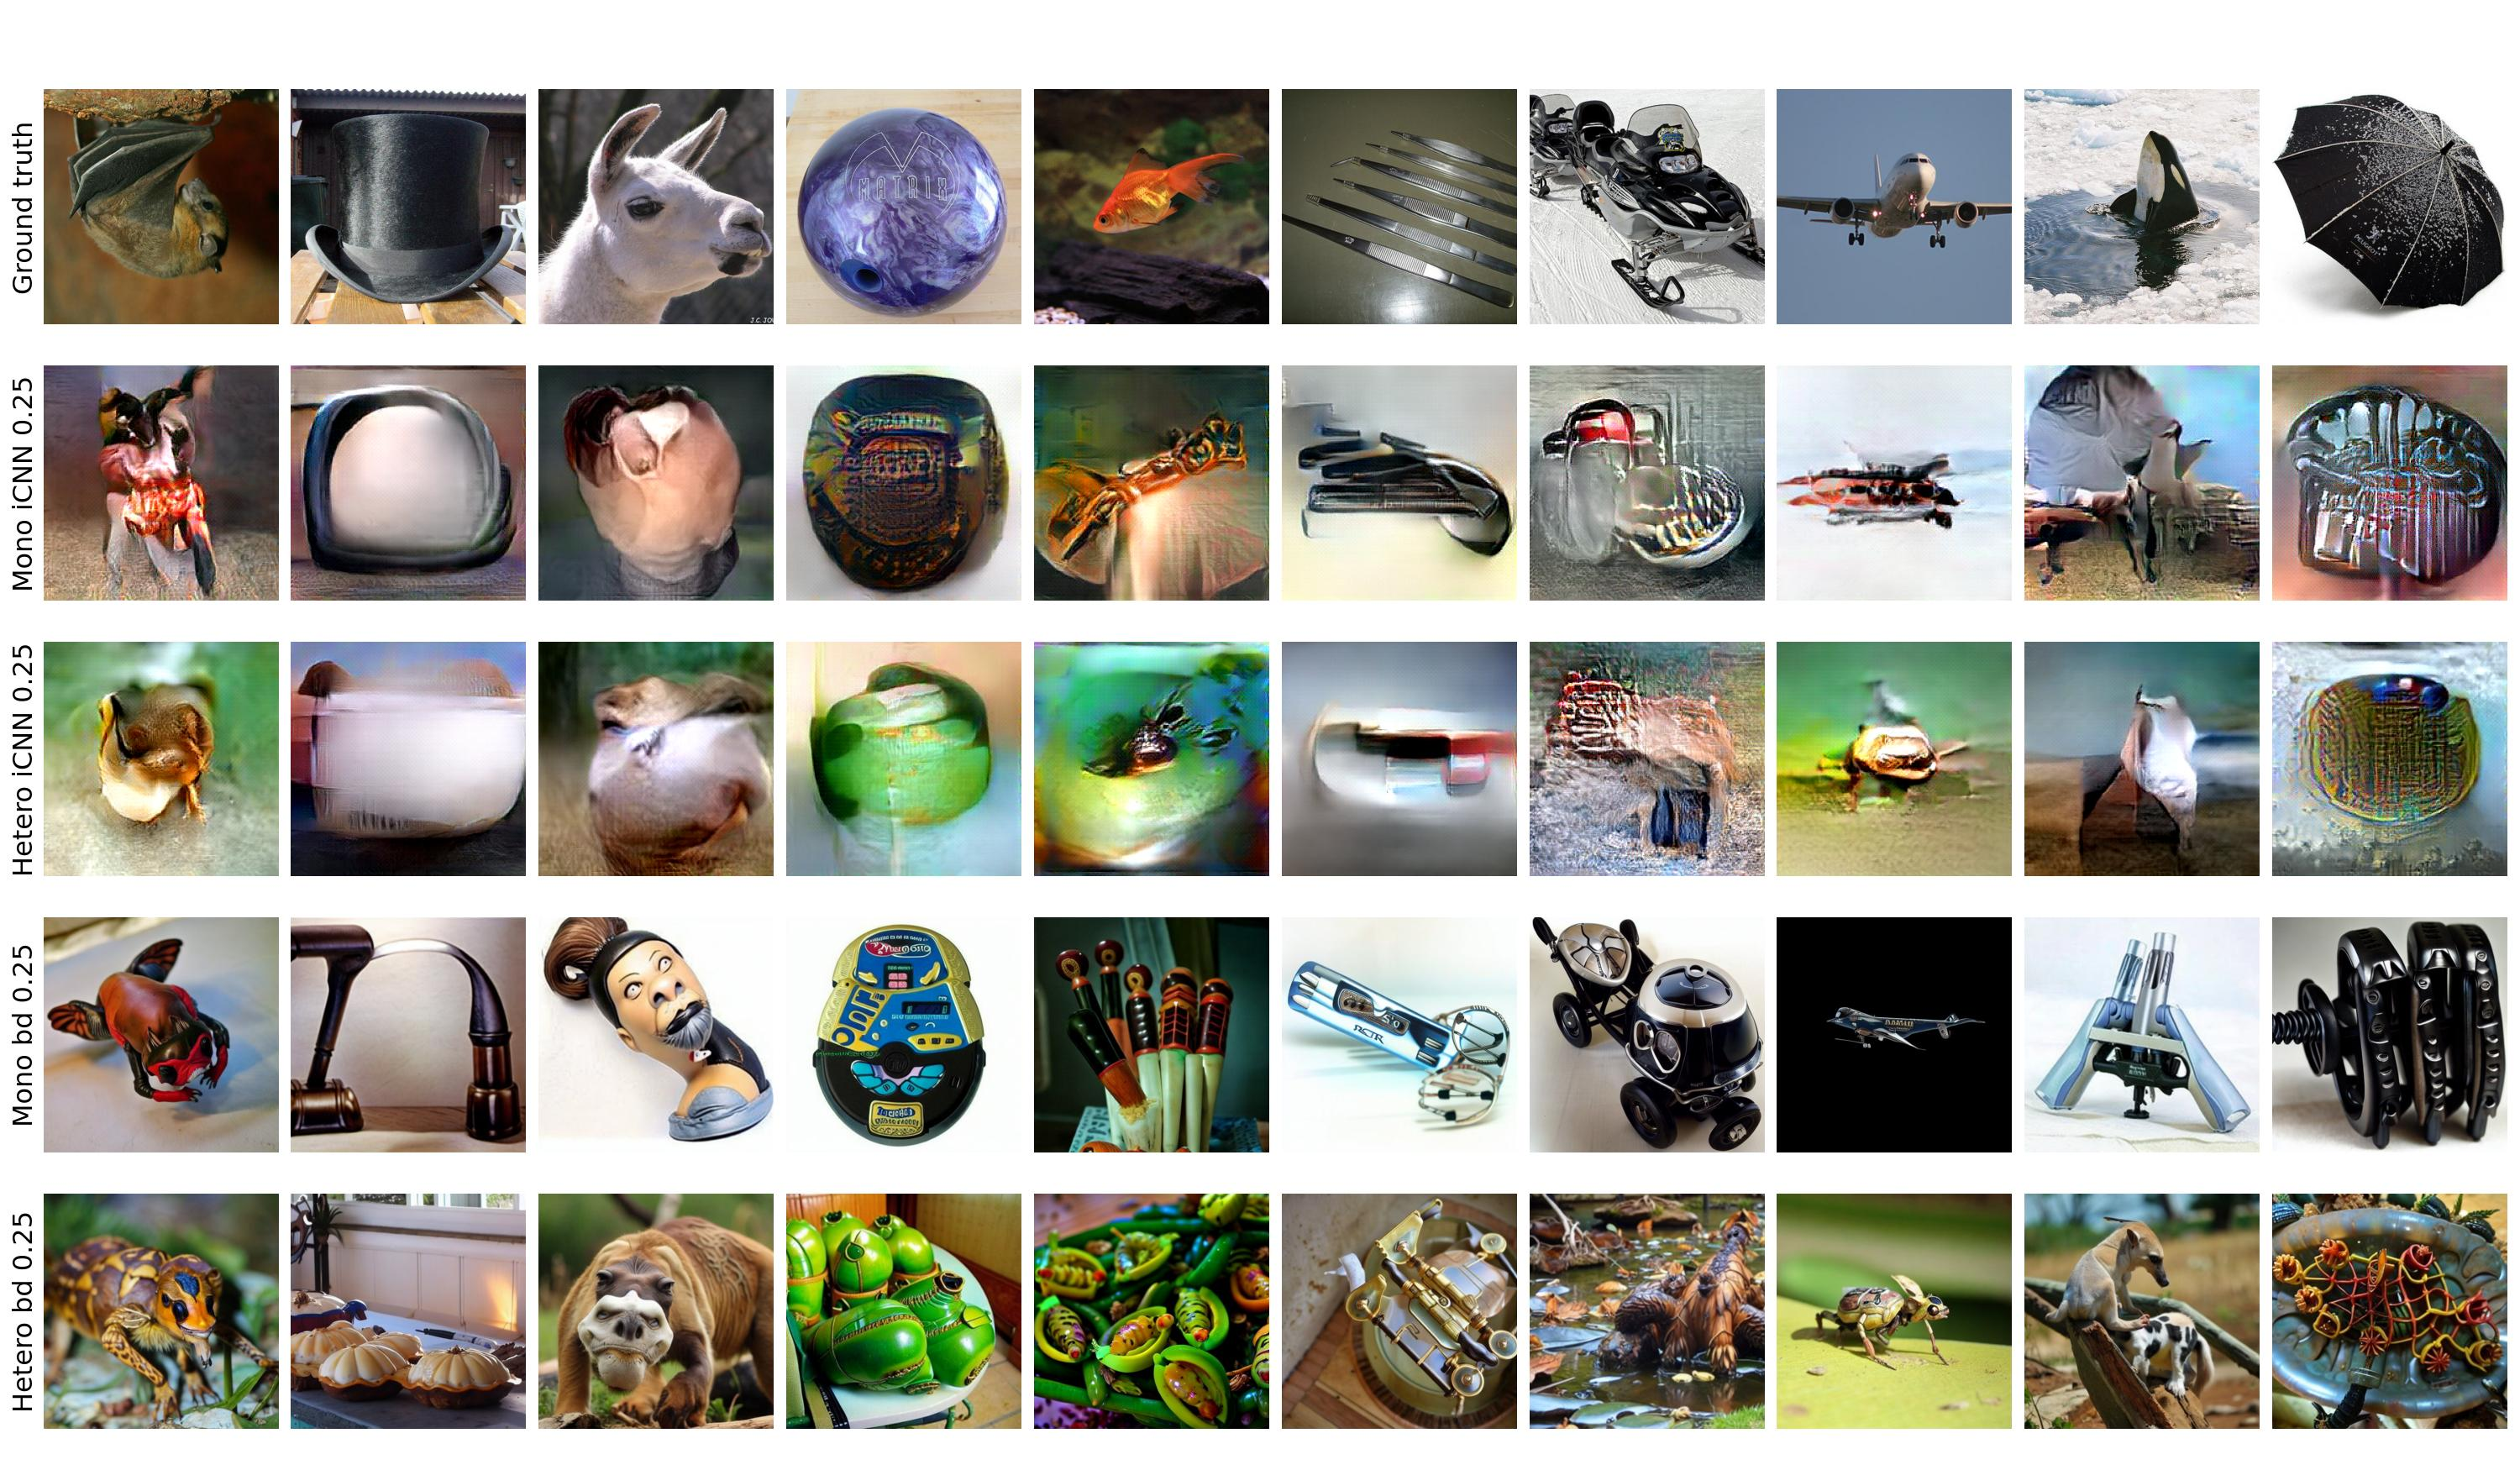
\includegraphics[width=1\textwidth]{plots/dropout_discussion_test.JPEG}
  \caption[Reconstructed images monotone vs.\ heterogeneous training samples]{Qualitative results for monotone vs.\ heterogeneous training images on natural test images. The top row depicts the ground truth image. Each following row depicts the reconstruction where the translator was trained using the dropout strategy and reconstruction algori defined on the left side (Note: bd stands for Brain-Diffuser).}\label{fig:dropout_discussion_test}
\end{figure}

\subsubsection{Future directions}

The results of the dropout experiment showed that the diversity of the training data set can have a significant influence on the \rOne{translation} of brain activity and the reconstruction of images. However, the exact direction and nature of the influence on the  reconstructions is still unclear. The results of this study were inconclusive in this respect. Further research is needed on the influence of the diversity of training images on brain \rOne{activity translation}. To this end, further different types of dropout could be used. For example, it is possible to use dropout based on the actual semantic categories (e.g.\ using the stimulus code), so that the results do not depend on the UMAP embedding and random initial conditions during clustering. Furthermore, a more sophisticated algorithm could be used to separate the monotonous from the heterogeneous images that also includes semantic information. 

One limitation of the study is that subsampling is only possible top-down. This means that a large data set is required, which is first reduced. Ideally, there would be a way to evaluate the quality of an existing subsample iteratively from a bottom-up perspective  to determine what an image should look like that needs to be added to the dataset to improve the performance. One possibility could be an active learning approach~\cite{senerActiveLearningConvolutional2018, guoDeepCoreComprehensiveLibrary2022}, which could be used during training to always look for the next image that improves the performance. Ultimately, the aim of this research is to investigate how the nature of a dataset needs to be in order to optimise reconstruction performance. For instance an approach like the one of Couch et al.~\cite{couchSizeClassBalance2024} could be used, that measures the dataset quality/diversity in a single metric. These results could then be used to create optimised training data sets that can be shown to subjects in future MRI studies. This optimised training data set does not necessarily have to consist of a sub-sample of natural images. Dataset distillation~\cite{wangDatasetDistillation2018,yuDatasetDistillationComprehensive2024} could be used to create an artificial training dataset that is optimised to improve the \rOne{translation}, allowing higher generalisation to all possible test images. Further research is needed to determine how such an artificial training dataset might look like and whether, for example, it is necessary to show subjects natural training images at all or if it might be better to only show abstract, generated images. 

In summary, this experiment showed that diversity-based subsampling has an impact on reconstruction performance, but that this impact needs further investigation in terms of direction and exact magnitude. In particular, the Brain-Diffuser algorithm performed very poorly with the artificial shapes, and its \rOne{translator} performance improved only marginally even with a larger amount of training data (see the random dropout results). The following experiments therefore look for ways to improve the performance of the Brain-Diffuser, especially with artificial shapes.


\section{Experiment 2: Enhancing The Training Captions}
% Corresponging Progress Reports:
% https://www.notion.so/241220-Matthias-reducing-train-data-with-care-First-AI-captions-0a0a3c610dba4d9c84d4eda4fb1c53dd
% https://www.notion.so/250110-Matthias-AICaptions-Evaluation-053ef06c3e6e4858808c9266cc1bffc0
% https://www.notion.so/20250119-Matthias-Filling-The-gaps-2-a8f598e120de4b6ba4b20a7d0a2a9253#18e2cfd830264119bbfcd90d223b4cc0

\subsection{Background}

Ich muss auf jeden Fall die Hypothese aufstellen, dass sich die Rekonstruktionsleistung von Artificial Shapes erhöht wenn ein Augenmerk auf low-level Features in den captions drin ist und für natürliche Testbilder, wenn ein Augnemerkt auf den high-level Featuers in den captions drin ist. 

\subsection{Methods}
To further investigate the performance of the Brain Diffuser algorithm, the influence of the subtitles and the cliptext translator is first tested. Possible differences that may result from the high-level vs.\ low-level information of an image are to be analysed. For this reason, additional captions are created below for the training data, focusing on either the high-level or the low-level features of the image. The API of ChatGPT\cite{OpenAI_ChatGPT_2024} was used to generate the additional captions for the training images. With this, captions with two different prompts were generated for all 1200 training images. As it was empirically found that the cliptext features can encode less information with increasing number of tokens (= caption length)\cite{zhangLongCLIPUnlockingLongText2024}, care was taken to ensure that the length of the generated captions did not exceed 35 tokens as far as possible. The two prompts used to generate the subtitles are as follows
\begin{itemize}
    \item \textbf{high-level}: Describe the visual contents of this picture. Focus on the semantic concepts in the image. What are the main subjects of the image and what is happening in it? Make sure the output doesn't exceed 25 tokens.
    \item \textbf{low-level}: Describe the visual contents of this picture without using the word representing its direct category or semantic meaning as much as possible. Instead, focus on the colors, shapes, and textures with their relative positions in the image. Do not interpret the scene just describe what is actually visible. Make sure the output doesn't exceed 25 tokens.
\end{itemize}

The number of desired tokens per generated caption can only be specified implicitly via the prompt, without cutting off a caption in the middle. Accordingly, the number of tokens actually generated varies slightly. Captions longer than 35 tokens were excluded and the prompt was repeated until a corresponding caption shorter than 35 tokens was found. On average, 30.81 tokens (std = 2.8) were generated for the low-level captions and 22.84 (std = 3.17) for the high-level captions. The higher length of the low-level captions can be explained by the fact that semantic concepts, which can usually bundle many low-level properties (e.g. `dog' vs. `creature with four legs, fur and snout'), have to be avoided. Figure~\ref{fig:aicap_caption_samples} compares the high-level and low-level captions for two images from the training dataset with the human-generated captions. It can be seen that the low-level captions do indeed largely avoid semantic descriptions and tend to describe colours, shapes and textures. The high-level captions are comparatively similar to the human-generated captions and refer to semantic concepts (e.g.\ raccoon or can).

\begin{figure}[ht]
    \centering
    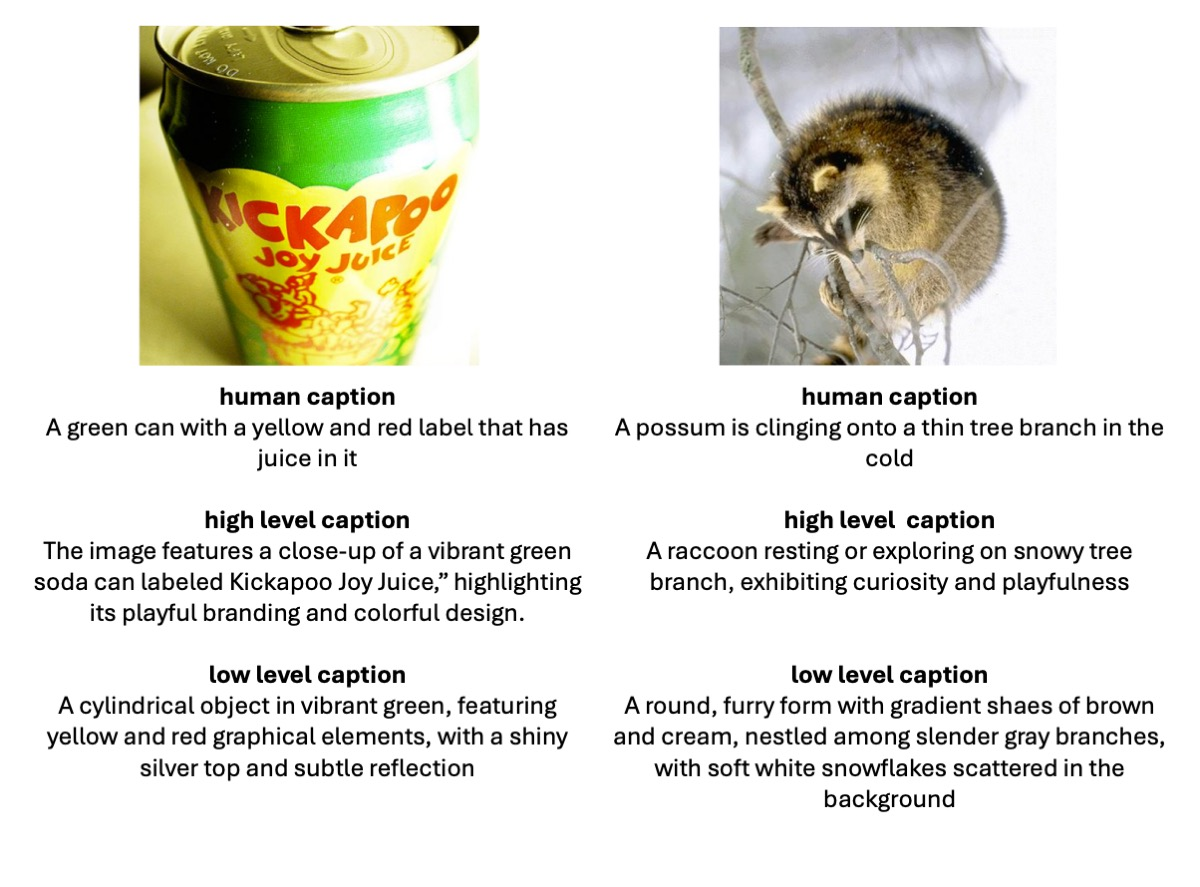
\includegraphics[width=1\textwidth]{plots/aicap_samples.jpeg}
    \caption{Captions with different prompts}\label{fig:aicap_caption_samples}
\end{figure}

The generated captions were subsequently used to train the Brain Diffuser's cliptext encoder. The clipvision and VDVAE components of the brain-diffuser do not change as a result, so only the performance of the cliptext translator is reported. For an extended baseline against which to compare the AI-generated subtitles, the human-generated subtitles are shuffled in an additional test condition. Thus, in this condition the captions have nothing to do with the actual image content, the translator should not be able to learn to make any meaningful predictions, just as the reconstructions produced with the translator trained with shuffled captions should be worse than with the normal baseline. In the Translator, the human-generated captions are used as test data for all comparisons to ensure comparability between conditions (i.e.\ the same test data is used for all conditions). 

When reconstructing with the Versatile Diffusion algorithm in the Brain Diffuser, the mixing parameter, which determines the influence of the cliptext features on the final reconstruction, is set to 0.4 and 0.8 respectively. In the original publication of the brain-diffuser\cite{ozcelikNaturalSceneReconstruction2023} the mixing parameter was 0.4, but in order to obtain a stronger influence of the captions and thus to be able to better evaluate the differences in the captions, the reconstructions are additionally analysed here with the parameter 0.8.


\subsection{Results}

\subsubsection{Translator Performance}

\begin{figure}[ht]
    \centering
    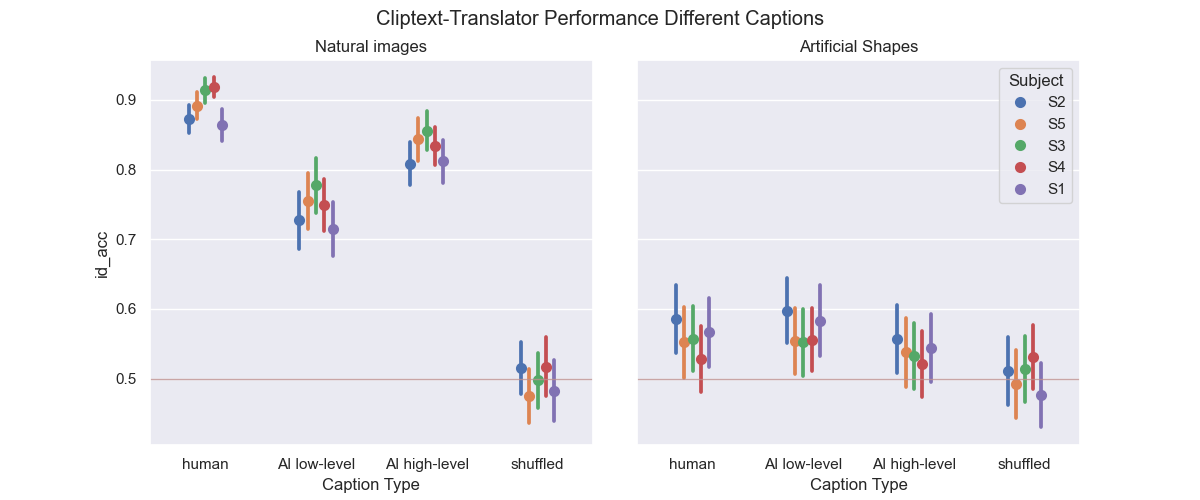
\includegraphics[width=0.9\textwidth]{plots/aicap_translator.png}
    \caption{AI-cap translator}\label{fig:aicap_translator}
\end{figure}

Figure~\ref{fig:aicap_translator} shows the results of the cliptext translator for both the natural test images and the artificial shapes. The effects can be seen very clearly for the natural test images, the identification accuracy of the translator trained with the human-generated captions is the highest. This is not surprising, as the test data for all conditions were also the human-generated captions of the test images, and therefore there is a slight domain mismatch for the AI data captions (the training data is generated by the AI, the test data by humans). The translator trained with shuffled training data is exactly at random probability, so the cliptext features could rightfully not be predicted. Both conditions with the AI-generated test data are also significantly better than random probability, with the high-level captions performing slightly better than the low-level captions (as noted above, the high-level captions also have a higher agreement with the human-generated captions). 


The results for artificial shapes are very different. Again, shuffled training data can predict results only at the random level; all other translators also show improved performance compared to the shuffled test data (and thus improved performance compared to the random level). In this condition, however, the translators trained with AI-generated high-level captions perform worse than those trained with low-level captions. The translator trained on the human-generated captions also appears to outperform the AI-generated high-level captions, although the result is somewhat less clear. 

\subsubsection{Reconstruction Performance}


The quantitative performance of the reconstructions for the natural test images is shown in Figure~\ref{fig:aicap_reconstruction_test_both_mixings} and for the artificial shapes in Figure~\ref{fig:aicap_reconstruction_art_both_mixings}. The results for mixing parameters 0.4 and 0.8 are shown for each type of caption and metric. The natural test images show that the differences between the individual captions with a mixing parameter of 0.4 are very small. Even the reconstructions with shuffled captions are only slightly worse with a mixing of 0.4 than with valid captions. The differences only become apparent when comparing the results with a mixing of 0.8. First, it can be observed that the pixel correlation increases for all captions as the mixing parameter increases. This is the case even for shuffled captions. An increased influence of the cliptext features therefore increases the pixel correlation in any case, even if it is a semantically incorrect influence as in the case of the shuffled captions. In the case of Dreamsim and Clip Accuracy, on the other hand, performance decreases as the mixing  increases, especially in the case of shuffled captions. For human-generated captions and high-level captions, performance degrades less with increasing mixing (or even remains constant) than for low-level captions. 
\begin{figure}[ht]
    \centering
    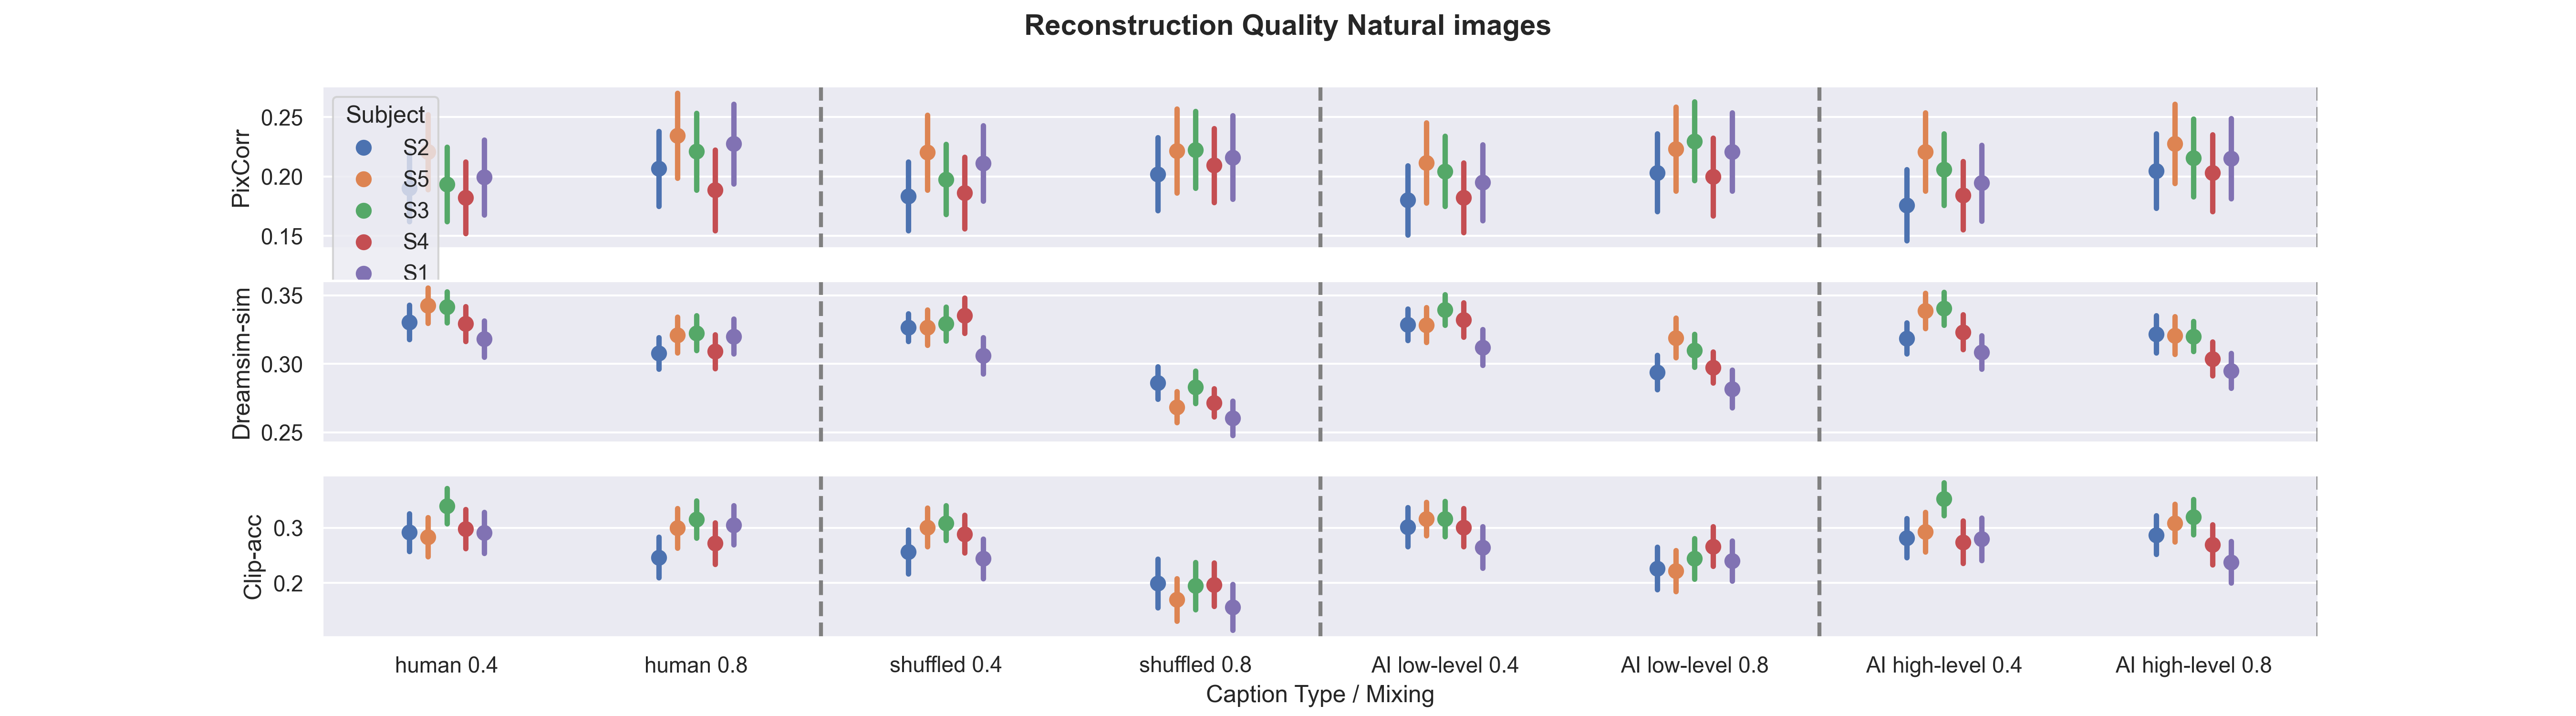
\includegraphics[width=1\textwidth]{plots/aicap_reconstruction_test_both_mixings.png}
    \caption{Reconstruction Natural Test Images with different captions}\label{fig:aicap_reconstruction_test_both_mixings}
\end{figure}


As before with the Translator, the results of the reconstruction of the artificial images are reversed. Again, with a low mixing of 0.4, there are very only few observable differences between the captions. And also as before, the pixel correlation increases with increasing mixing for all captions. But now, compared to the natural test images, the performance measured with Dreamsim Similarity also increases with increasing mixing for all captions. Especially with low level captions, good performance can be achieved with artificial images when mixing is high. The results for human and high-level captions are relatively similar and still significantly better than shuffled captions. The results for clip accuracy are very low and therefore difficult to interpret, as there is generally little semantic content in the artificial images, so the result is not surprising. 

\begin{figure}[ht]
    \centering
    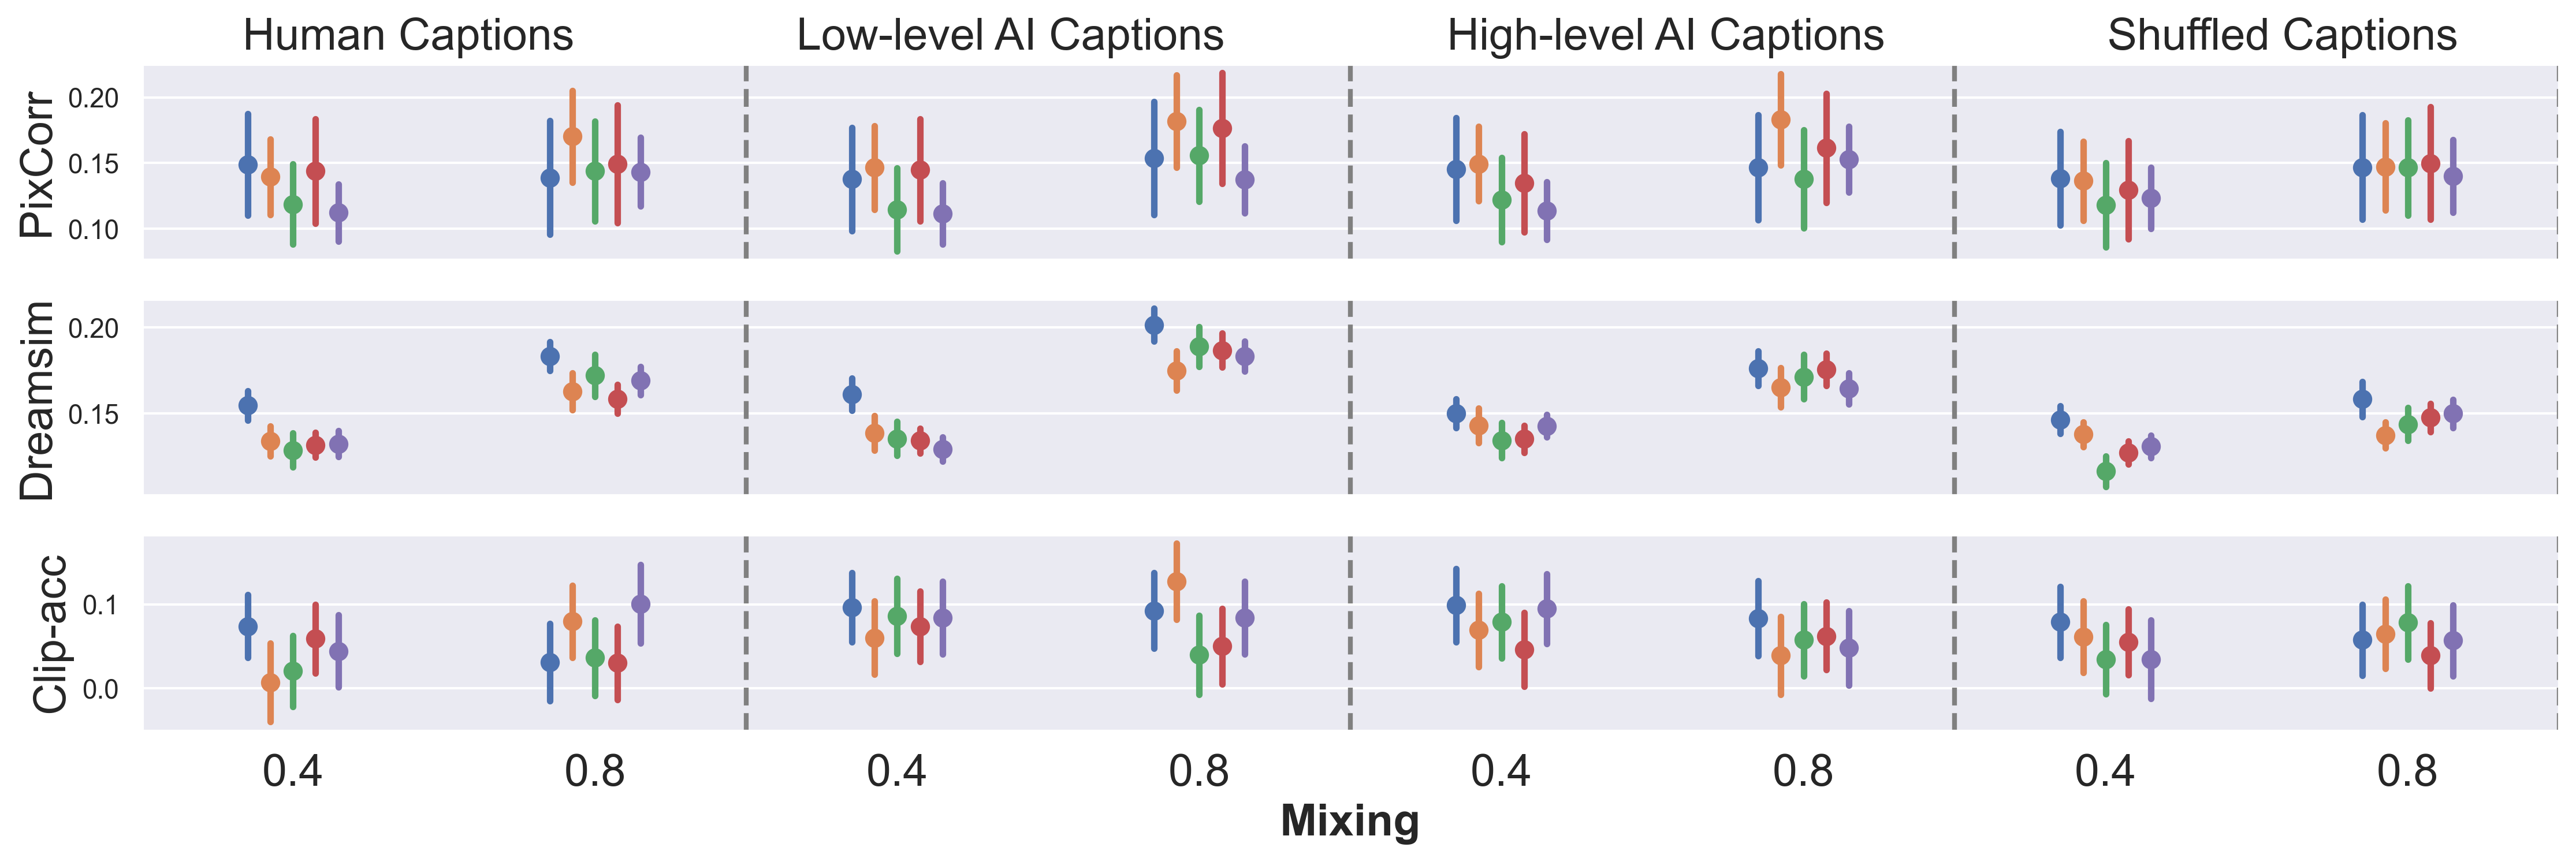
\includegraphics[width=1\textwidth]{plots/aicap_reconstruction_art_both_mixings.png}
    \caption{Reconstruction Artificial Images with different captions}\label{fig:aicap_reconstruction_art_both_mixings}
\end{figure}


% \begin{figure}[ht]
%     \centering
%     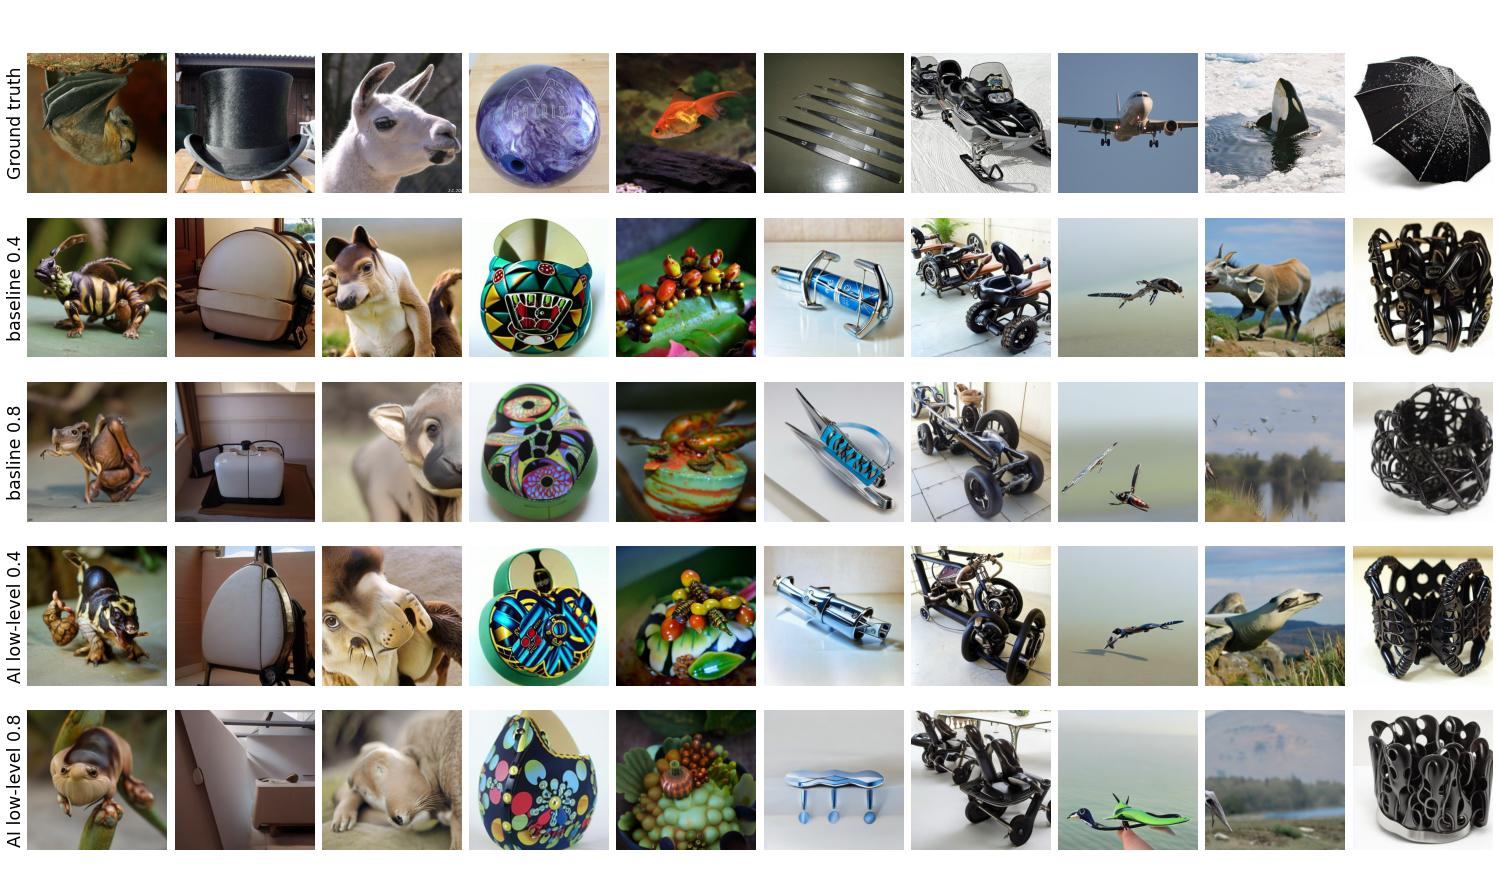
\includegraphics[width=0.6\textwidth]{plots/aicap_qual_test.JPEG}
%     \caption{AI-cap Reconstructions Natural Test Images}\label{fig:aicap_qual_test}
% \end{figure}

% \begin{figure}[ht]
%     \centering
%     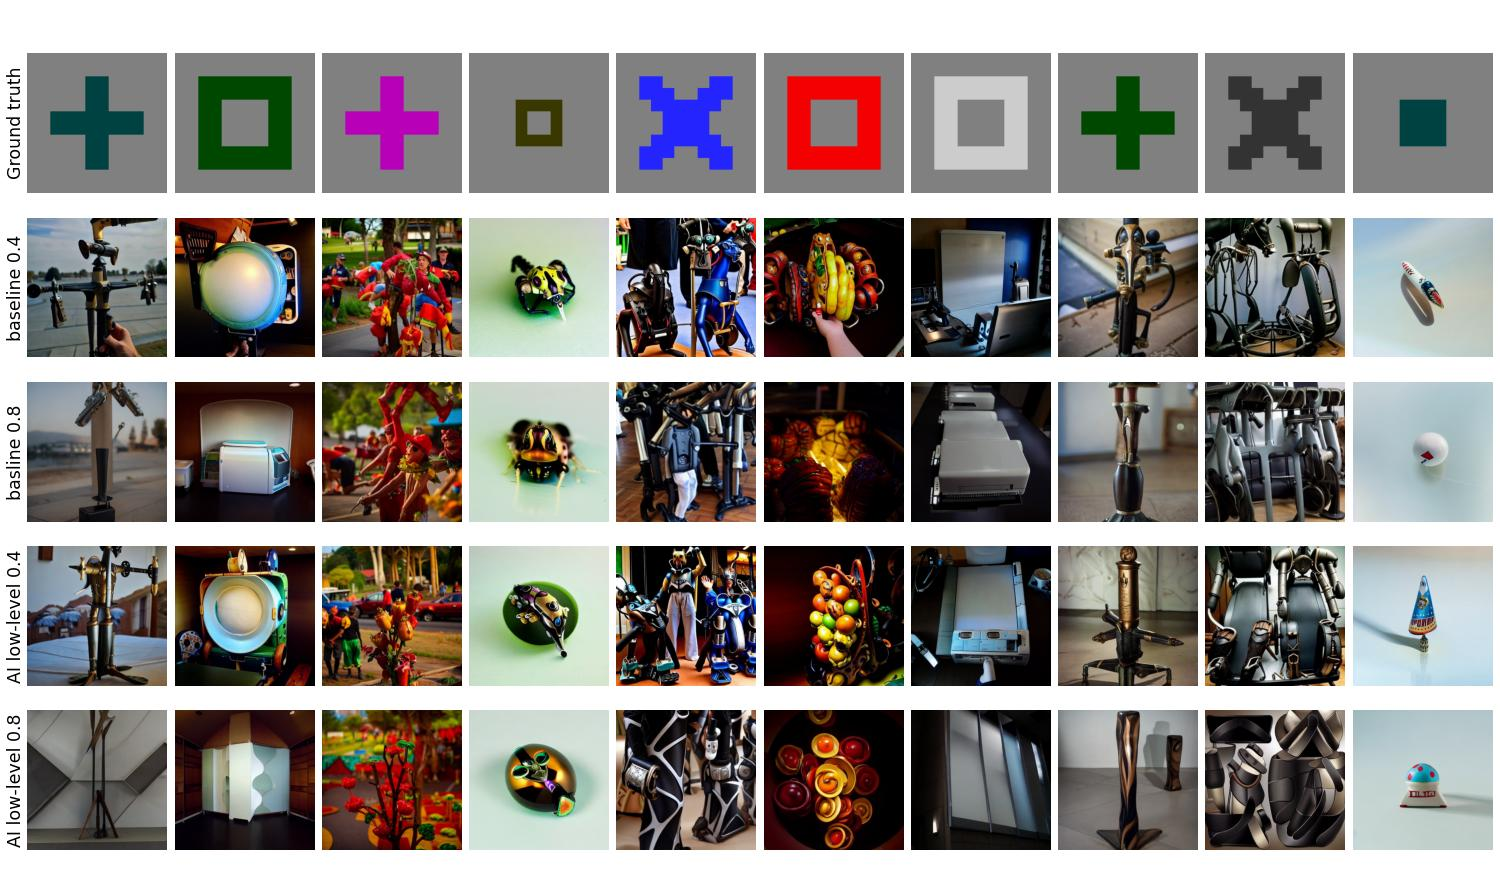
\includegraphics[width=0.6\textwidth]{plots/aicap_qual_art.JPEG}
%     \caption{AI-cap Reconstructions Artificial Shapes}\label{fig:aicap_qual_art}
% \end{figure}

\subsection{Discussion}

It could be shown that different types of captions, which refer to different features of the image, have a heterogeneous influence on the reconstruction performance. On the one hand, this confirmed the hypothesis that captions in the training data that refer to low-level features of the images can also ensure that the artificial shapes (which themselves do not carry much high-level information) can be better reconstructed. On the other hand, the reconstruction performance for natural images (which carry a lot of semantic meaning) was not reduced,  when the labels referred to the high-level information of the training images. PixelCorrelation did not prove to be a particularly good metric in this experiment, as it was able to detect an improvement in performance with increasing mixing in all cases (even with shuffled captions). The Dreamsim metric, on the other hand, best demonstrated the effect described above (low-level captions are good for artificial shapes and bad for natural test images). 

\begin{figure}[ht]
    \centering
    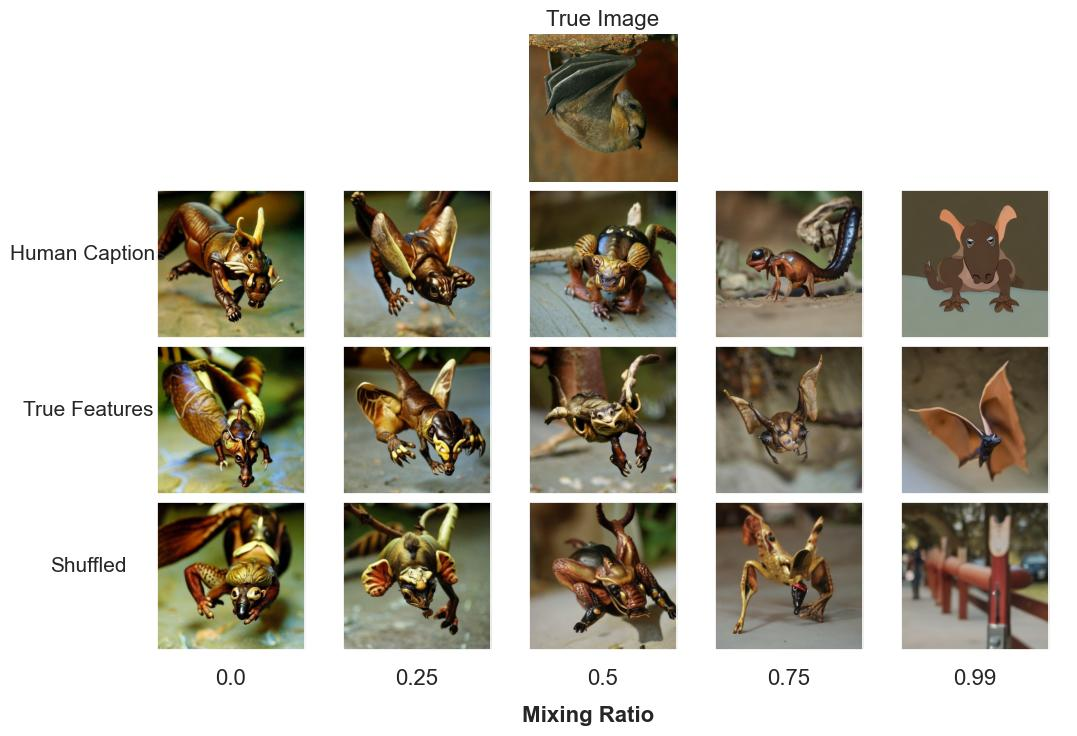
\includegraphics[width=0.8\textwidth]{plots/aicap_reconstruction_evolution_test_0.JPEG}
    \caption{AI-cap Reconstructions Artificial Shapes}\label{fig:aicap_reconstruction_evolution_test_0}
\end{figure}

For the natural test images and the artificial images, contrary effects were found as to whether increased mixing degrades (natural images) or improves (artificial shapes) the reconstruction performance. In order to identify the reason for this, a further analysis focused on the mixing parameter was conducted. Figure~\ref{fig:aicap_reconstruction_evolution_test_0} (and in the appendix in Figure~\ref{fig:aicap_reconstruction_evolution_art_0}) shows reconstructed images with increasing mixing ratios. In addition to the human and shuffled captions, the true features (i.e.\ the extracted clip text features of the images) are also used. It can be seen that as the mixing ratio increases, there is less detail in the image and the result becomes more blurred. This could be the explanation for the fact that the reconstruction performance (measured with dreamsim) for the natural test images decreases as the mixing ratio increases: because there is less detail in the reconstructed images, the naturalness (TODO quote) of the images decreases and they are less reminiscent of photorealistic images (the effect of the decreasing performance is shown quantitatively in Figure~\ref{fig:aicap_reconstruction_quant_evolution_test} in the appendix). This could also be the reason why the performance for the artificial images generally increases as the mixing ratio increases: because there is less (hallucinated) detail in the reconstructed images, the similarity to the low-detail artificial images increases (the increasing performance for the artificial images is shown in a quantitative manner Figure~\ref{fig:aicap_reconstruction_quant_evolution_art} in the appendix).



TODO: Überleitung dahin, dass mit den Captions der semantische Wert nicht besonders erhöht werden konnte, der Peak bei 0.4 erreicht ist, mit cliptext also nicht bedeutent die semantische Abbildung erhöht. Deshalb wollen wir an den anderen Teil vom Brain-difuser ran, clipvision. 
TODO: Add some qualitative Results for the 0.8 mixing (maybe also add 0.95 mixing) for the artificial shapes

 \chapter{Discussion}
% https://www.scribbr.com/dissertation/discussion/

% Summary: A brief recap of your key results
% Interpretations: What do your results mean?
% Implications: Why do your results matter?
% Limitations: What can’t your results tell us?
% Recommendations: Avenues for further studies or 

In this work, three experiments were performed to investigate the influence of diversity on image reconstruction from brain activity. The two algorithms iCNN by Shen et al.~\cite{shenDeepImageReconstruction2019} and in particular the Brain-Diffuser by Ozcelic et al.~\cite{ozcelikNaturalSceneReconstruction2023} were investigated in more detail. The specific results of the individual experiments have already been discussed. At this point, we will discuss the experiments and the resulting findings in the broader context of data diversity and output dimension collapse. First, the individual results are briefly summarised to then open up the discussion for the broad context. In the first experiment, an attempt was made to create subsamples of the training data that maximised diversity at different levels (low-level to high-level features) and tested against a random selection of the training data. For the iCNN in particular, a diversity-based selection of training data slightly improved the reconstruction for the natural test images, but the reconstruction of the artificial shapes was slightly worsened by the diversity-based subselection, indicating a deterioration of the OOD generalisation. A more detailed investigation, using more monotonous or heterogeneous subsamples for training, revealed important findings: on the one hand, the brain diffuser may be very strongly influenced by the monotonous images (or its performance in reconstructing the artificial shapes was largely based on the monotonous test images). On the other hand, the iCNN appeared to have a slight bias towards reconstructing images with single objects in the foreground and little detail in the background, such as the artificial shapes. In the second experiment, the influence of the CLIP text embeddings on the brain diffuser reconstruction was analysed. AI was used to create additional captions for the training images, focusing on either low-level or high-level features of the images. These captions were used to train the CLIP text translator and subsequently create reconstructions with the brain diffuser. Particularly at high levels of mixing, i.e. when the CLIP Text features had a stronger influence on the reconstruction, it was shown that a focus on the low-level features ensured a better reconstruction of the artificial images. At the same time, however, the performance of the natural test images was reduced. Finding a setting that improves both OOD generalisation (in the form of artificial images) and the performance of congruent test images therefore seems difficult. However, these results at least imply that focusing on low-level vs.\ high-level features during training may also favour corresponding reconstructions. In the third experiment, the influence of the CLIP vision embeddings on the reconstruction of the brain diffuser was further investigated. Backpropagation was used to craft perturbations in the training images, which are barely visible to the naked eye, but strongly alter the meaning of the CLIP vision embeddings extracted from them. The information from the captions could thus be added to the images in the form of `semantic noise'. The CLIP Vision translator was trained on these perturbed images, and reconstructions were again produced using the Brain Diffuser. It was found that the reconstructions could not be improved for the natural test images by focusing on the semantic meaning, nor could they be improved for the artificial shapes by reducing the semantic meaning of the images. In fact, performance deteriorated in both conditions. This raised the question of whether a perturbation in which the modified images had to be similar to the originals was necessary at all, and whether modifying the CLIP vision features directly might be a more targeted and effective way of modifying the semantic meaning of the images.

% In dieser Arbeit wurden drei Experimente durchgeführt, die den Einfluss von Diversität auf die Rekonstruktion von Bildern aus Gehirnaktivität untersucht haben. Dabei wurden die zwei Algorithmen iCNN von Shen et al.~\cite{shenDeepImageReconstruction2019} und insbesondere der Brain-Diffuser von Ozcelic et al.~\cite{ozcelikNaturalSceneReconstruction2023} näher untersucht. Die spezifischen Ergebnisse der einzelnen Experimente wurden bereits diskutiert. An dieser Stelle soll nun eine Diskussion der Experimente und der daraus folgenden Erkenntnisse im breiteren Kontext der Datendiversität und des output dimension collapse stattfinden. Zunächst seien dazu die einzelnen Ergebnisse kurz zusammengefasst beschrieben. 


% Im ersten Experiment wurde versucht Subsamples der Trainingsdaten zu erstellen, welche die Diversität auf verschiedenen Ebenen (low-level Features bis high-level Features) maximiert haben und gegen eine zufällige Auswahl der Trainingsdaten getestet. Insbesondere mit dem iCNN konnte mit einer diversitätsbasierten Auswahl der Trainingsdaten die Rekonstruktion für natürliche Testbilder leicht verbessert werden, die Rekonstruktion von den artificial Shapes hingegen wurde durch die diversitätsbasierte Subselection aber hingegen leicht verschlechtert, was auf eine Verschlechterung der OOD Generalisierung hindeutet. In einer näheren Untersuchung, in der weitere subsamples für das Training genutzt wurden die besonders monoton bzw. heterogen waren wurden wichtige Erkenntnisse sichtbar: einerseits lässt sich der Brain-Diffuser sehr stark von den monotonen Bildern beeinflussen (bzw. seine Leistung, die Artificial Shapes zu rekonstruieren basierte maßgeblich auf den monotone Testbildern). Andererseits stellte sich heraus, dass der iCNN einen leichten bias zu haben scheint, Bilder zu rekonstruieren, die wie die artificial shapes einzelne Objekte im Vordergrund und wenig Details im Hintergrund haben. 

% Im zweiten Experiment wurde der Einfluss der CLIP Text embeddings auf die Rekonstruktion des Brain-Diffusers untersucht. Mithilfe von KI wurden zusätzliche Captions der Trainingsbilder erstellt, die sich entweder auf low-level oder high-level features der Bilder fokussierten. Mithilfe dieser captions wurden CLIP Text translator trainiert und mit dem Brain-Diffuser Rekonstruktionen erstellt. Insbesondere bei hohem mixing, also stärkerem Einfluss der CLIP Text features bei der Rekonstruktion zeigte sich, dass ein Unterschied im Fokus auf die low-level Features für eine bessere Rekonstruktion der artificial images sorgte. Im gleichen Atemzuge wurde aber die Performance für die natural test images verringert. Ein setting zu finden, bei dem also sowohl die OOD Generalisierung (in Form der artificial images) als auch die Performance bei kongruenten Testbildern verbessert wird scheint also schwer zu sein. Diese Ergebnisse bedeuten aber zumindest, dass der Fokus auf low-level vs high-level features bei dem training auch korrespondierende Rekonstruktionen begünstigen kann.

% Im dritten Experiment wurde der Einfluss der CLIP Vision embeddings auf die Rekonstruktiond es Brain-Diffusers weiter untersucht. Mithilfe von backpropagation wurden gezielt perturbations in den Trainingsbildern erzeugt, die für das bloße Auge kaum sichtbar sind, aber die Bedeutung der daraus extrahierten CLIP Vision embeddings stark verändert haben. Die Informationen aus den Captions konnten so in Form von `semantic noise' den Bildern hinzugefügt werden. Mit diesen perturbed Bildern wurde der CLIP Vision translator trainiert und wieder mit dem Brain-Diffuser Rekonstruktionen erstellt. Es zeigte sich, dass die Rekonstruktionen weder für die natural test images verbessert werden konnte, wenn ein Fokus auf die semantische Bedeutung gelegt wurde, noch dass sie für die artificial shapes verbessert werden konnte, wenn die semantische Bedeutung der Bilder verringert wurde. Für beide Bedingungen wurde die performance sogar eher verschlechtert. Daraufhin stellte sich die Frage, ob eine perturbation bei der die modifizierten Bilder den originalen überhaupt ähnlich sein müssen überhaupt notwendig ist und nicht eventuell eine Modifikation der CLIP Vision features direkt eine zielgerichtetere und effektivere Möglichkeit sein könnte, die semantische Bedeutung der Bilder zu modifizierten.
The results in this paper largely support those of Shirakawa et al.~\cite{shirakawaSpuriousReconstructionBrain2024}. It could be reproduced that the diffusion-based brain diffuser does not perform particularly  with artificial shapes, and that the hallucinations of the diffusion process become visible strongly. As Shirakawa et al. also showed, the iCNN performed better for this test dataset. These results suggest that the reconstruction algorithm also has a strong influence on the generalisation ability of the reconstructions. Regarding the output dimension collapse, the experiments with the monotonic dropout and the low-level labels yielded interesting results: almost all of the performance of the brain diffuser with the artificial shapes seems to be due to the monotonic training images. This can be interpreted to mean that the 'monotone background' dimension in the training data is essential for these test images. This supports the results of the simulation study by Shirakawa et al. in the sense that training data in the right dimensions is needed to enable general reconstructions. The results with the low-level labels can be interpreted in the same way; a focus on low-level labels can also support the low-level reconstructions (artificial shapes). However, in both cases, due to the fact that no new data could be collected for this work, the performance on the natural test data decreased at the same time as the performance on artificial shapes increased. In order to gain further insight into whether the overall performance for all test data can be improved with the findings of this work, it would be important to create a new training data set that is designed specifically by regarding relevant image dimensions. Unfortunately, the question of which dimensions are fundamentally important for learning the reconstruction of the entire possible image space remains unanswered. The low-level vs. high-level and monotonic vs. heterogeneous dimensions analysed in this study are by no means the only possible dimensions that could be used. Other dimensions like colors, object categories, object locations, rotation and others that could possibly not even be described by natural language might also be suited better as the fundamental dimensions that would span the image space.

\cite{wangDiversityImageCaptioning2022}
- Diversity in Image captioning (ist vielleicht eher was noch fürs AICap Experiment)

Zu meinen Ergebnissen:
- PixelCorrelation ist nicht so gut (haben wir an vielen Ergebnissen schon irgendwie gesehen)
    - Zum Beispiel dass durch die Erhöhung von falschem Mixing die Ergebnisse verbessert wurden
    - Die random Reduction hat fast keinen Effekt gehabt
    - Schauen, wieso Brain-Diffuser überhaupt irgendwas von den Artificial Shapes rekonstruieren kann


den dimension collapse in dem monotone dropout ziemlich gut nochmal gesehen, es wird nur noch auf das abgebildet, was das modell schon kann
aber auch ein Bisschen catastrophic forgetting von yu et al 2023
Oder?
Also die Gesamtleistung wird ja dann nicht besser oder doch?
Also verglichen mit der main baseline frag ich mich gerade.
Sollte man vielleicht noch hinzufügen, also den Vergleich von monotone subsampling mit 100 baselin
\cite{wangDiversityImageCaptioning2022}
- Diversity in Image captioning (ist vielleicht eher was noch fürs AICap Experiment)

- Decoding von Brain-Diffuser ist auch irgendwo fraglich, weil das so wenig sensibel auf die random reduction war

Generell:
- https://x.com/PTenigma/status/1893459033379807586
- Erklärung dafür, dass der Brain-Diffuser in clip so viel besser ist, ist vielleicht einfach die image-naturalness
- Man könnte auch noch den tatsächlichen test einfügen in die versatile diffusion

Andere Datensätze:
- Things, NSD, jetzt neu auch NSD artificial images 
https://arxiv.org/pdf/2503.06286

Biologisch gesehen:
- Schauen, auf welchen gehirnebenen die Treatments von uns jeweils einen Effekt hatten und wo nicht.

Konkrete Veränderung des setups das wir haben:

- Andere "fertige" End2End-Algorithmen (mindeye etc.)
    - Man könnte auch komplette captions generieren lassen und nicht nur die Features wie bei unibrain \cite{maiUniBrainUnifyImage2023}

- Andere Decoder Algorithmen 
    - Statt der ridge regression, durch Methoden in dieser Arbeit könnten teilweise die Menge der Daten deutlich erhöht werden, wodurch möglicherweise auch etwas anderes als eine (Ridge) Regression verwendet werden könnte

- Andere Reconstruction Algorithmen:
    - Um die rare concepts zu verbessern sagen \cite{samuelGeneratingImagesRare2024} dass man sich vor allem auf den diffusion input fokussieren muss
        - man kann noch einen Schritt weiter gehen und sagen, man solle sich ausschließlich auf den Input konzentrieren und mehr mit VDVAEs machen (oder ähnlichen Algorithmen die nicht so viel halluzinieren)
    - Andere Image generation Algorithms (innerhalb des Brain-Diffuser Algorithm, also versatile diffusion austauschen)
    - Theoretisch sind viele Contexts möglich bei dem versatile diffusion approach, mit einer weiterentwicklung könnte man so dann auch je nach image das regeneriert werden soll ganz unterschiedlichen kontext geben (das schreibe ich auch schon teilweise beim aicap Experiment)
    - Generell kann man ja schauen, wie (ja wie nur, ich hab den Satz nicht fertiggeschrieben...)
    - iCNN mit clip ginge ja theoretisch auch
    - Oder Autoregressive models wie jetzt jüngst von OpenAI gezeigt wurde


Eventuell abschließen damit, dass die visuelle Verarbeitung so komplex und top-down reguliert ist, dass es wahrscheinlich bei der Bildrekonstruktion nicht eine einzige Wahrheit gibt. Klar, man kann versuchen ein Bild was jemand sieht 1zu1 wieder darzustellen, das wird aber der Verarbeitung im Kopf nicht unbedingt gerecht. Es können mehrere Unterschiedliche Repräsentationen gleichzeitig geschehen und damit unterschiedliche Bilder gleich gut rekonstruiert werden. 


\section{Conclusion}
% https://www.scribbr.com/dissertation/write-conclusion/
Hier nochmal die Zusammenfassung dessen was ich gemacht habe. 


% Clearly state the answer to your main research question
% Summarize and reflect on your research process
% Make recommendations for future work on your thesis or dissertation topic
% Show what new knowledge you have contributed to your field
% Wrap up your thesis or dissertation

% \include{chapter2}
% \include{chapter3}
% \include{chapter4}


%%% Appendicies of thesis  %%%%%%%%%%%%%%%%%%%%%%%%%%%%%%%%%%%%%%%%%%%%%%%%%%%%%%%%%%%%%%%%%%%%%%%%

\appendix
% From mitthesis package
% Version: 1.01, 2023/07/04
% Documentation: https://ctan.org/pkg/mitthesis

\chapter{Experiments}
\section{Dropout Experiment}


\begin{figure}[ht]
   \centering
   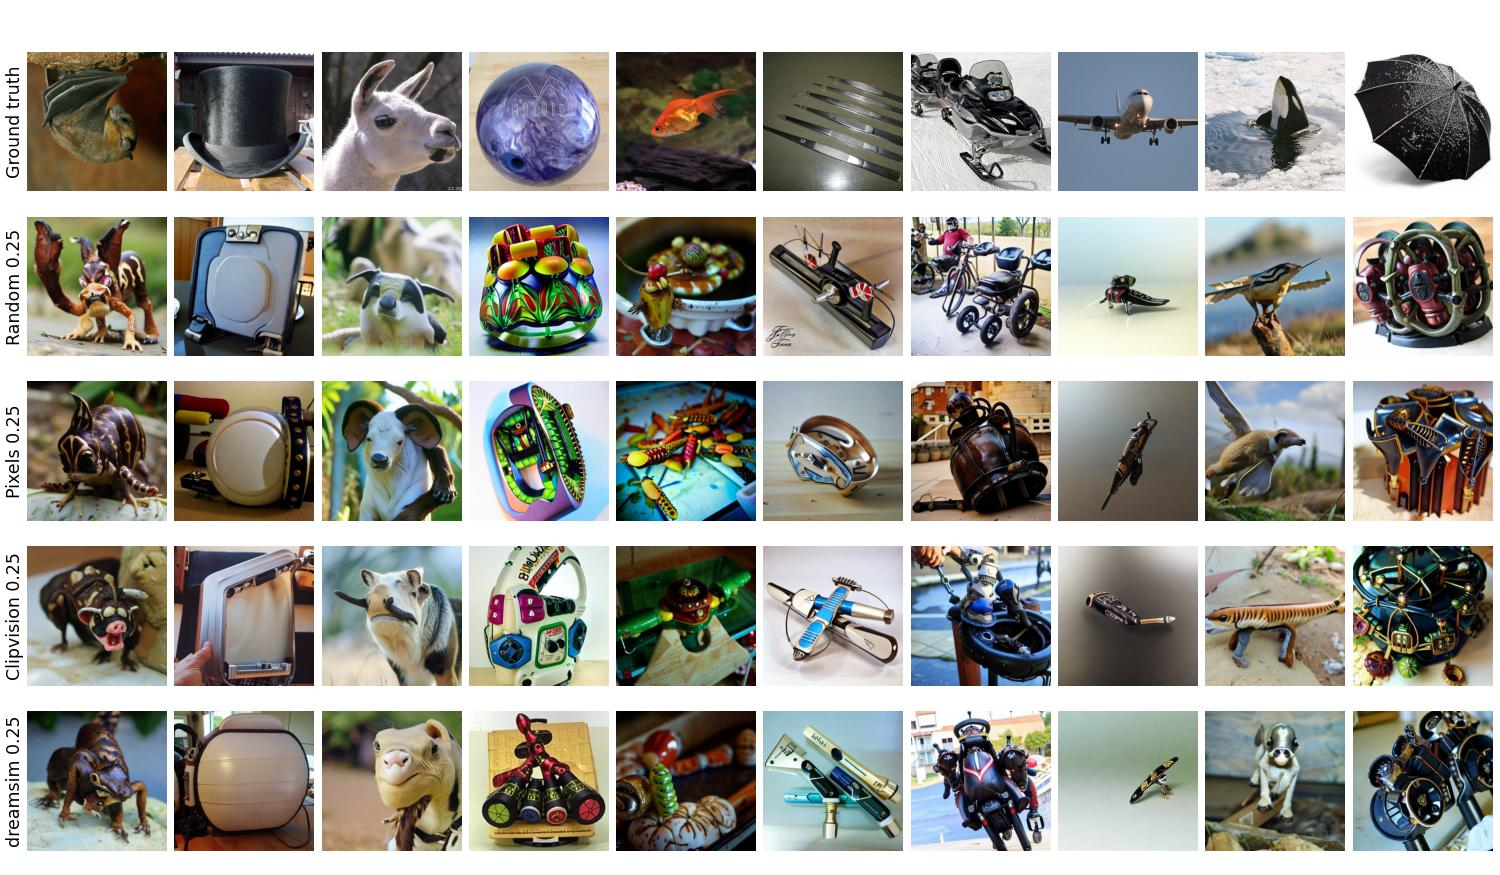
\includegraphics[width=1\textwidth]{plots/dropout_qual_eval_bd_test.JPEG}
   \caption{A nice image}\label{fig:dropout_qual_eval_bd_test}
\end{figure}

\begin{figure}[ht]
   \centering
   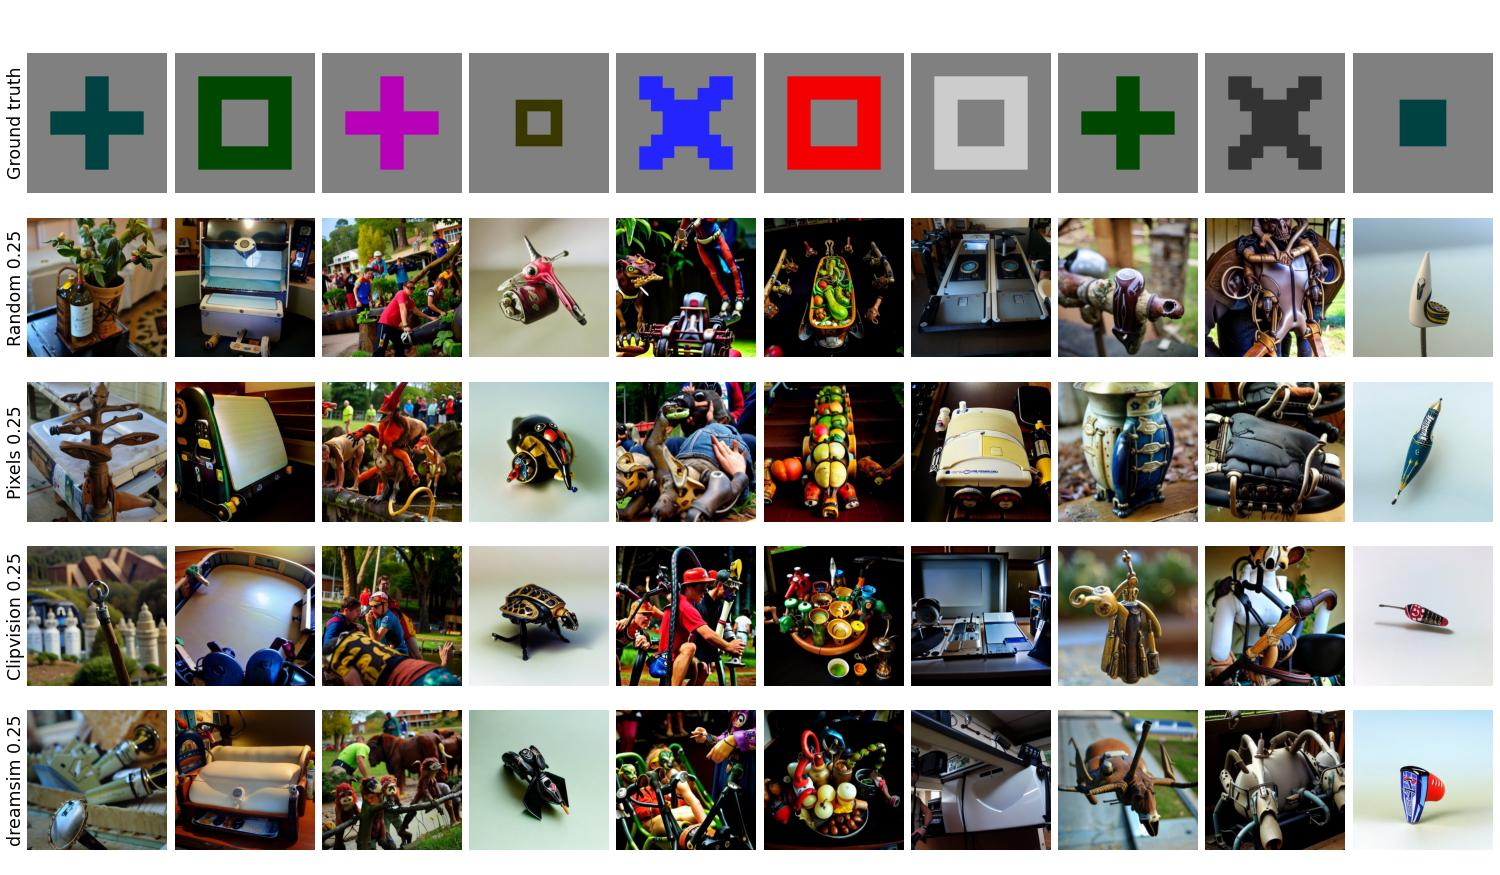
\includegraphics[width=1\textwidth]{plots/dropout_qual_eval_bd_art.JPEG}
   \caption{A nice image}\label{fig:dropout_qual_eval_bd_art}
\end{figure}

\section{Ai Captions}
\begin{figure}[ht]
   \centering
   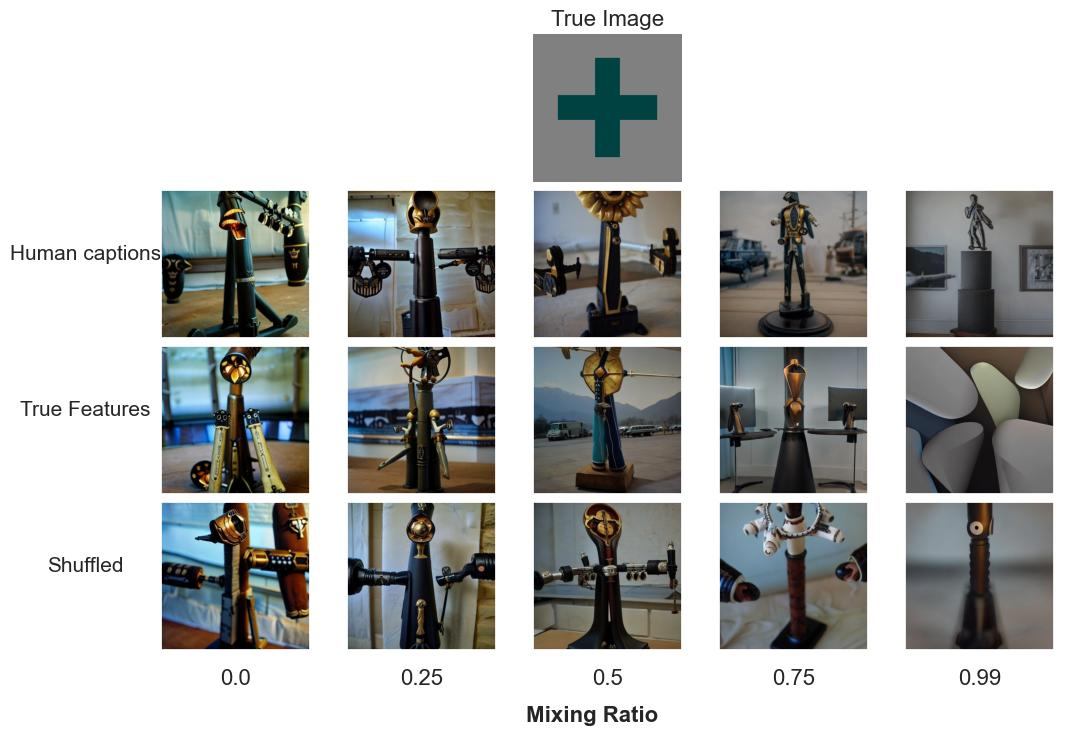
\includegraphics[width=1\textwidth]{plots/aicap_reconstruction_evolution_art_0.JPEG}
   \caption{AI-cap Reconstructions Artificial Shapes}\label{fig:aicap_reconstruction_evolution_art_0}
\end{figure}

\begin{figure}[ht]
   \centering
   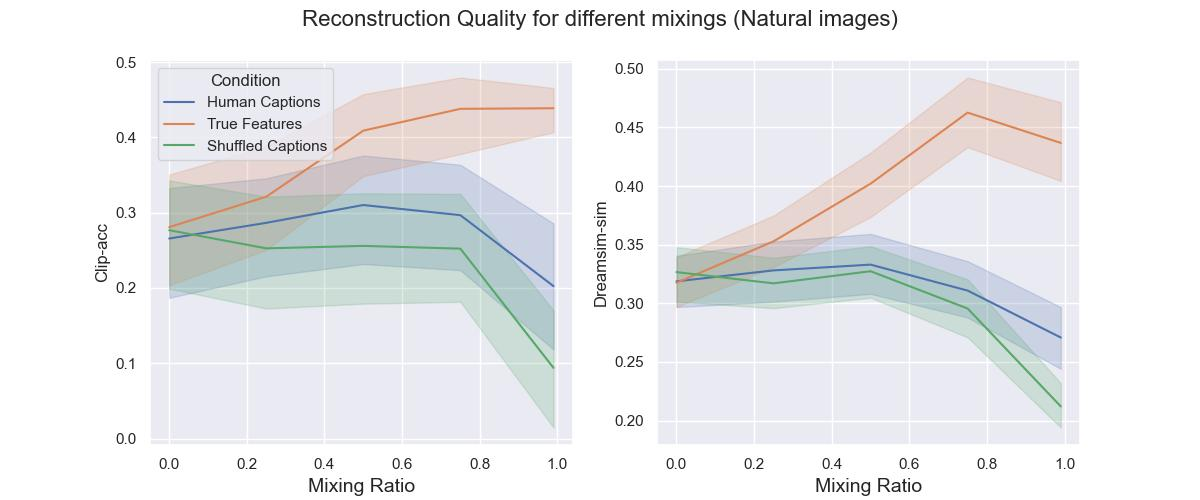
\includegraphics[width=1\textwidth]{plots/aicap_reconstruction_quant_evolution_test.JPEG}
   \caption{AI-cap Reconstructions Artificial Shapes}\label{fig:aicap_reconstruction_quant_evolution_test}
\end{figure}

\begin{figure}[ht]
   \centering
   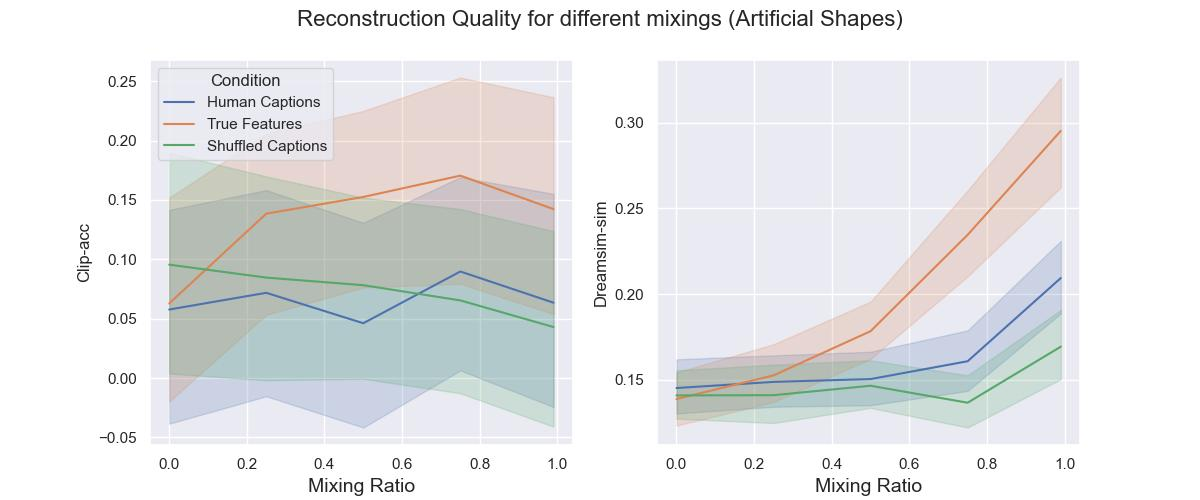
\includegraphics[width=1\textwidth]{plots/aicap_reconstruction_quant_evolution_art.JPEG}
   \caption{AI-cap Reconstructions Artificial Shapes}\label{fig:aicap_reconstruction_quant_evolution_art}
\end{figure}

\section{Perturbations}
\begin{figure}[ht]
    \centering
    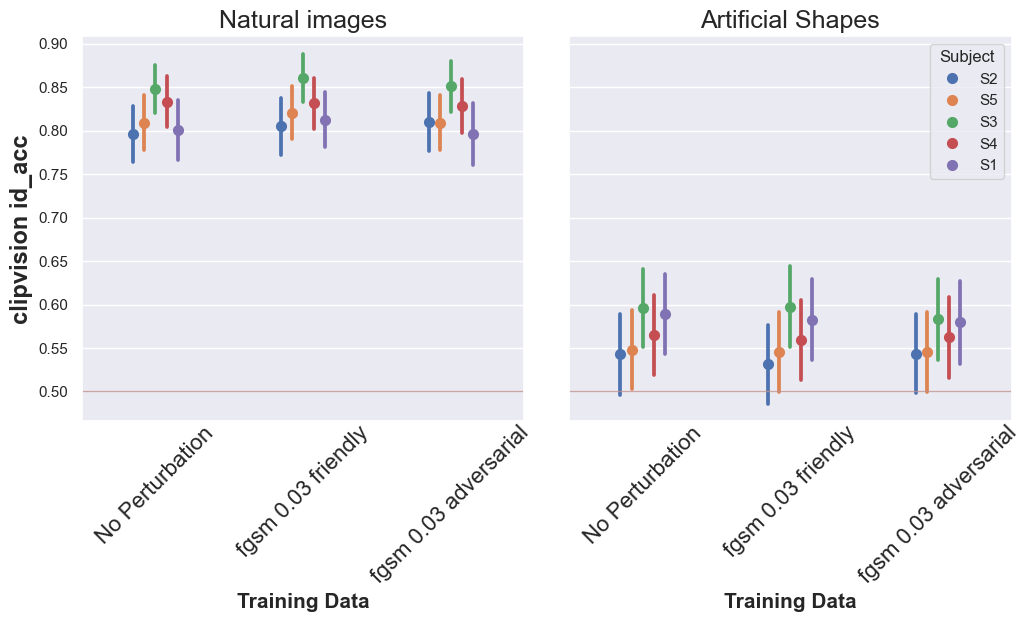
\includegraphics[width=1\textwidth]{plots/advpert_translator_fgsm_0.03.png}
    \caption{A nice image}\label{fig:advpert_translator_fgsm_0}
\end{figure}


\begin{figure}[ht]
    \centering
    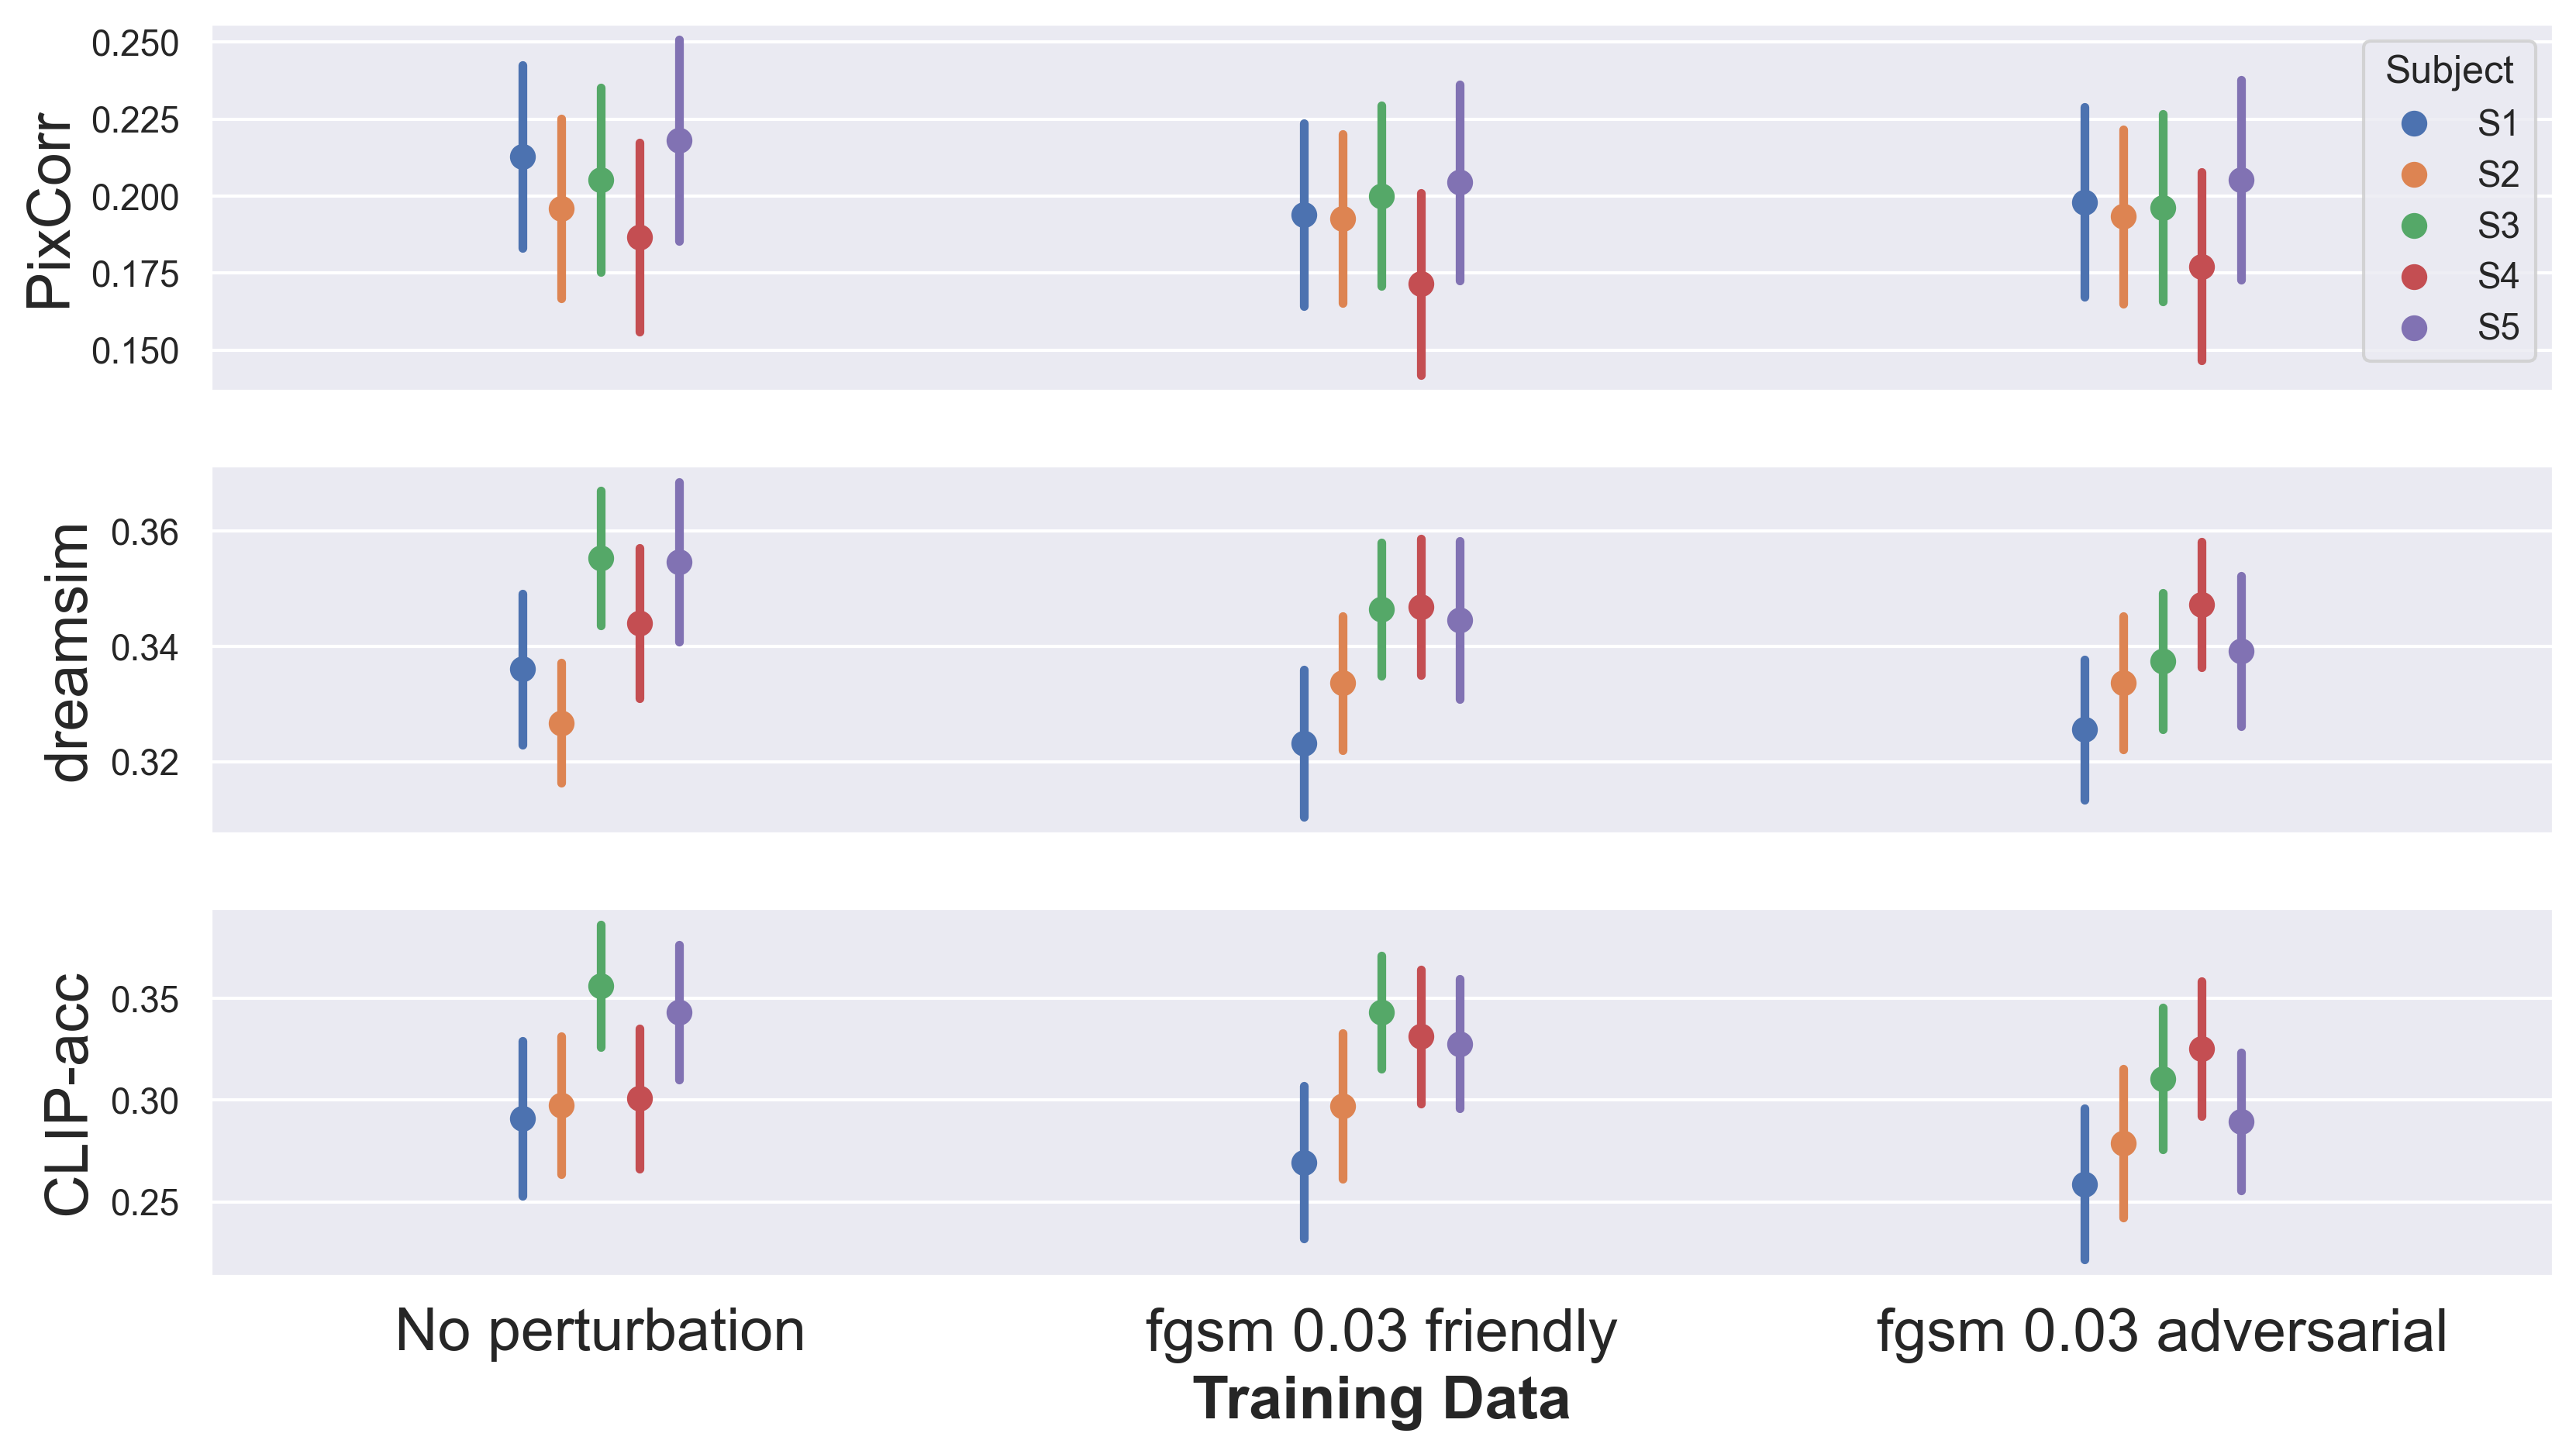
\includegraphics[width=1\textwidth]{plots/advpert_reconstruction_test_fgsm_0.03.png}
    \caption{A nice image}\label{fig:advpert_reconstruction_test_fgsm_0.03}
\end{figure}

\begin{figure}[ht]
    \centering
    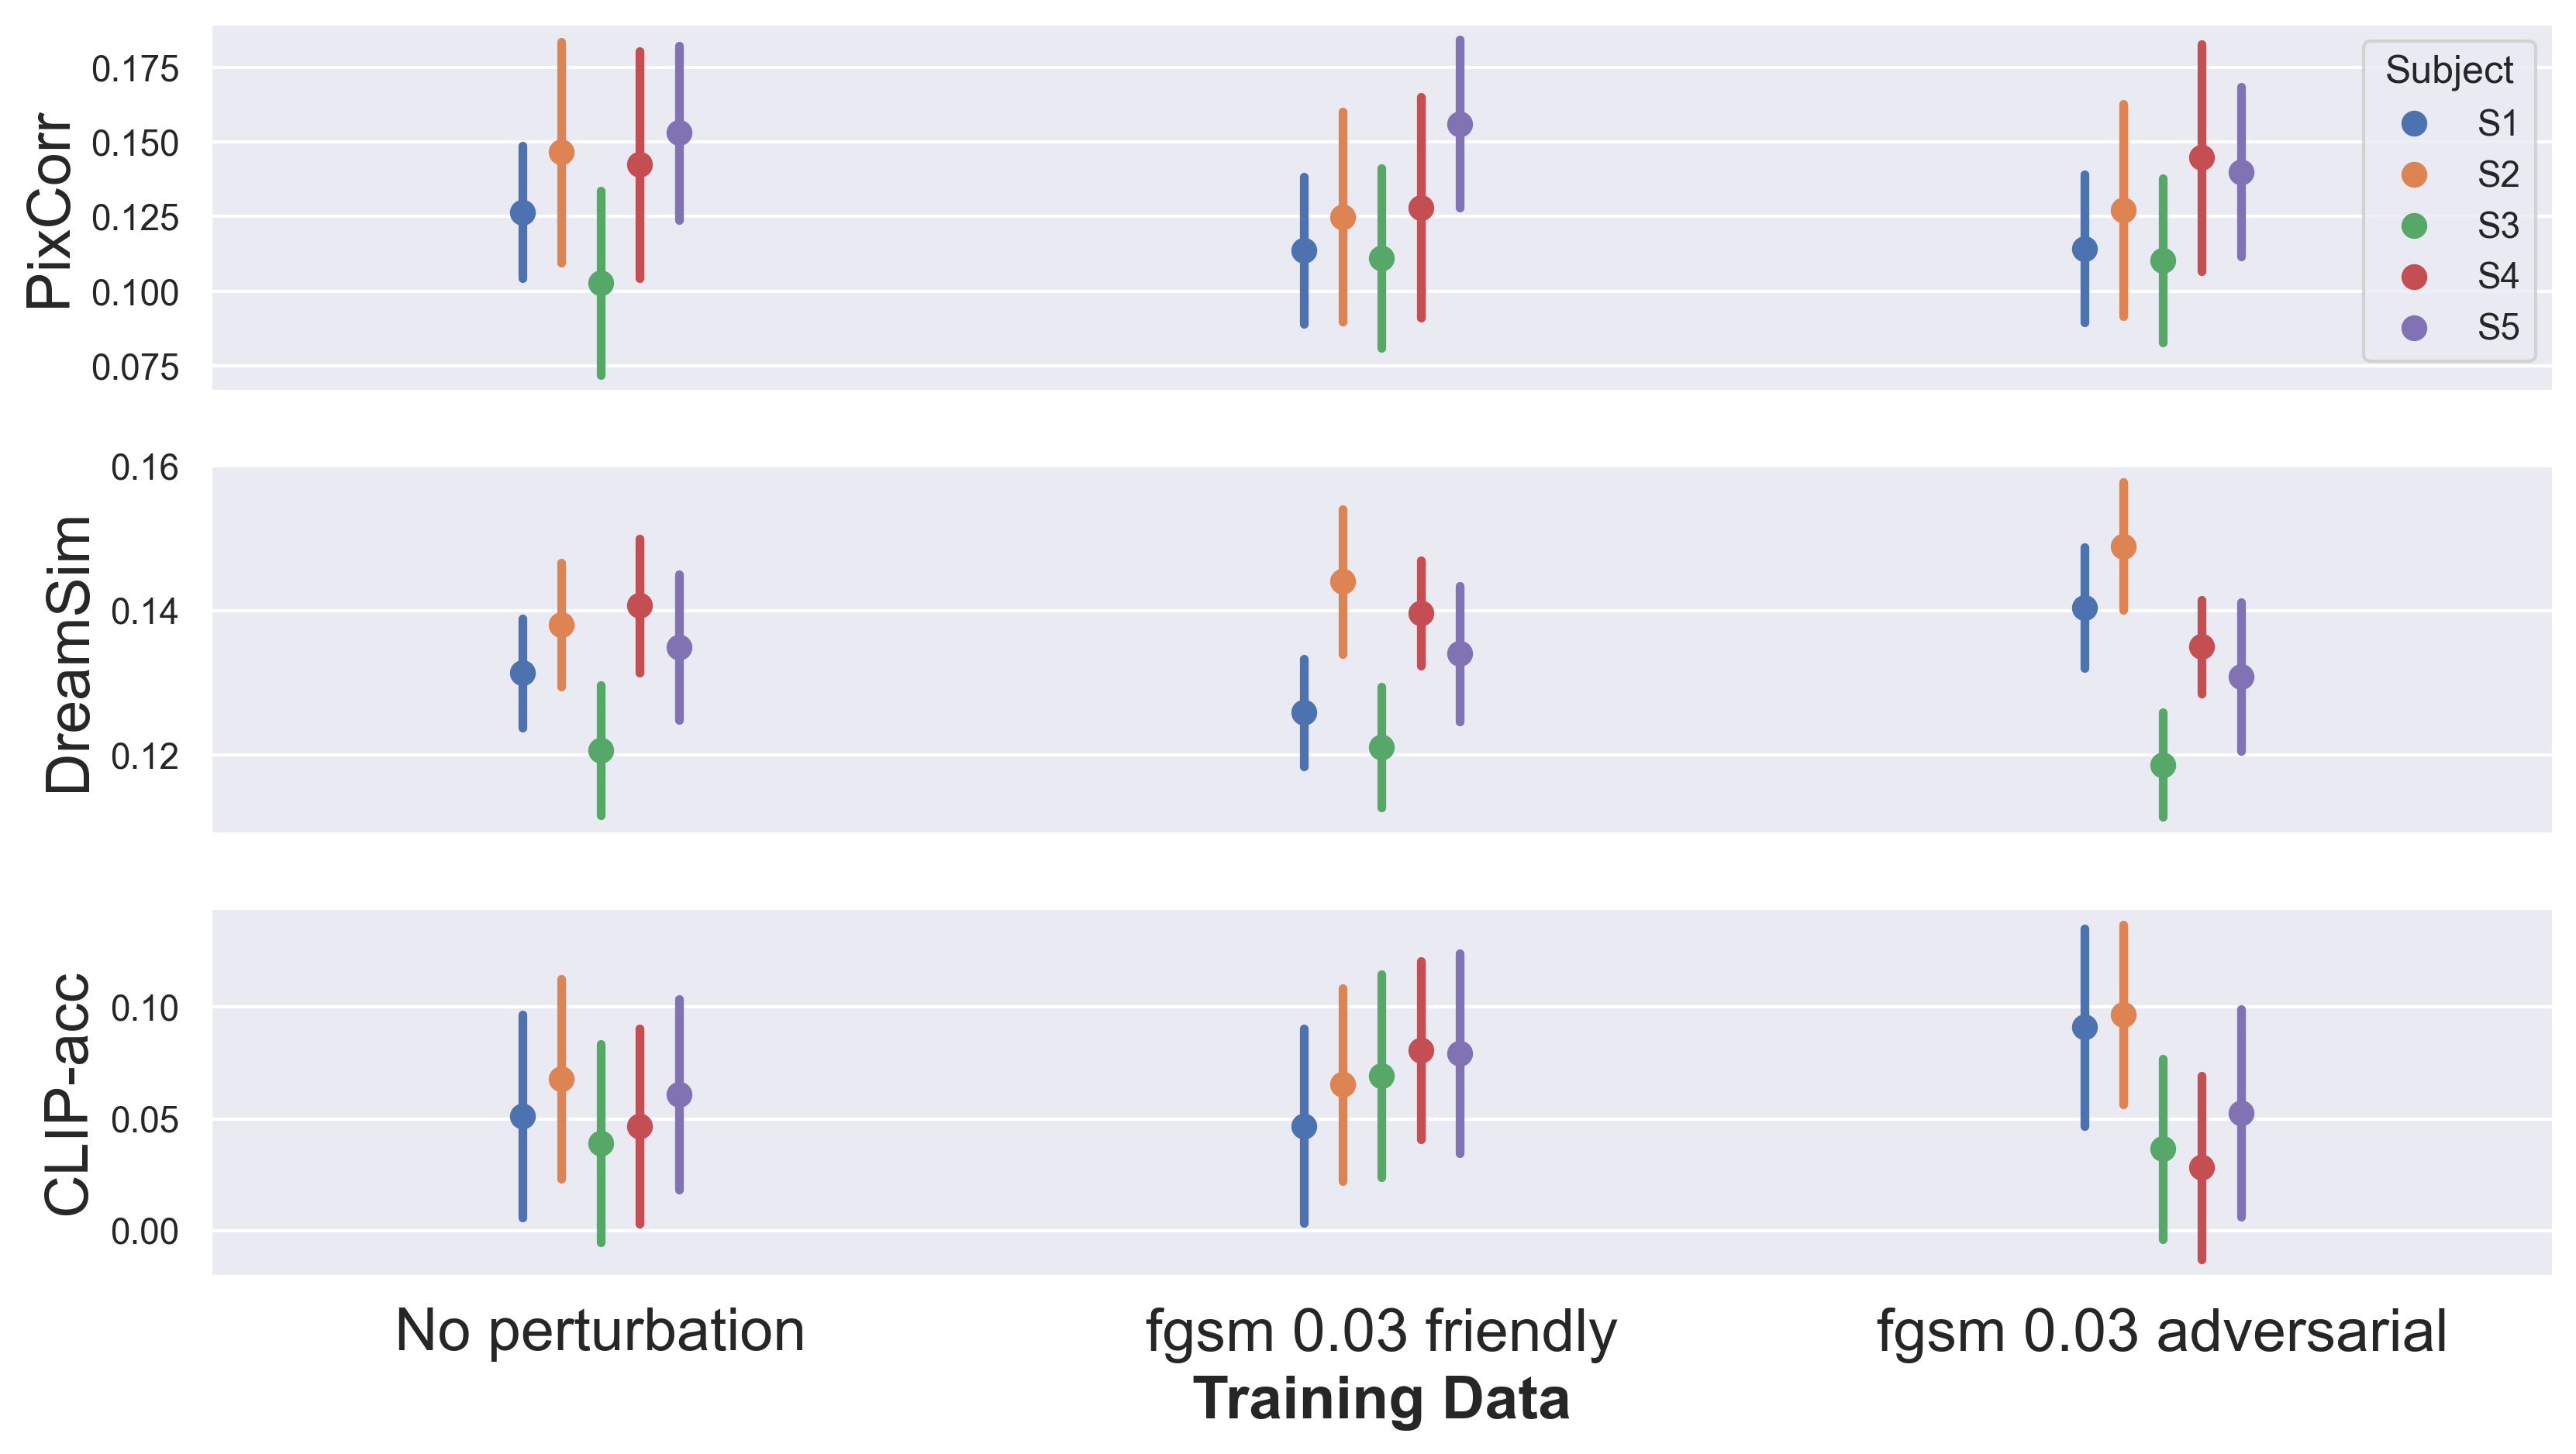
\includegraphics[width=1\textwidth]{plots/advpert_reconstruction_art_fgsm_0.03.png}
    \caption{A nice image}\label{fig:advpert_reconstruction_art_fgsm_0.03}
\end{figure}


% \chapter{Code listing}

% This example uses the \texttt{listings} package.

% \bigskip

% \lstdefinestyle{mystyle}{
%     backgroundcolor=\color{CadetBlue!15!white},   
%     commentstyle=\color{Red3},
%     numberstyle=\tiny\color{gray},
%     stringstyle=\color{Blue3},
%     basicstyle=\small\ttfamily,
%     breakatwhitespace=false,         
%     breaklines=true,                 
%     numbers=left,                    
%     numbersep=5pt,                  
%     showspaces=false,                
%     showstringspaces=false,
%     showtabs=false,                  
%     tabsize=2
% }%
% \lstset{language=[5.3]Lua,style={mystyle}}%

% \begin{lstlisting}
% function print_rate(kappa,xMin,xMax,npoints,option)
%      local c = 1-kappa*kappa
%      local croot = (1-kappa*kappa)^(1/2)
%      local logx = math.log(xMin)
%      local psi = 0
     
%      local xstep = (math.log(xMax)-math.log(xMin))/(npoints-1)
     
%      arg0 = math.sqrt(xMin/c)
%      psi0 = (1/c)*math.exp((kappa*arg0)^2)*(erfc(kappa*arg0)-erfc(arg0))
     
%      if option~=[[]] then
%   		 tex.sprint("\\addplot+["..option.."] coordinates{") 
%   		 -- addplot+ for color cycle to work
%      else
%   		 tex.sprint("\\addplot+ coordinates{")
%      end
%      tex.sprint("("..xMin..","..psi0..")")
     
%      for i=1, (npoints-1) do
%   		 x = math.exp(logx + xstep)
%   		 arg = math.sqrt(x/c)
%   		 karg = kappa*arg
%   		 if karg<5 then 
% 		 -- this break compensates for exp(karg^2), which multiplies the error in the erf approximation...
%   		    logpsi = -math.log(croot) + karg^2 + math.log(erfc(karg)-erfc(arg))
%   		    psi = math.exp(logpsi)
%   		 else
%   		    psi = (1/(karg) - 1/(2*(karg^3)) + 3/(4*(arg^5)) )/(1.77245385*croot)
%   		    -- this is the large x asymptote of the reaction rate
%   		 end
%   		 logx = math.log(x)
%   		 tex.sprint("("..x..","..psi..")")
%      end
%      tex.sprint("}")
% end
% \end{luacode*}
% \end{lstlisting}

% %% MIT Thesis class sample appendix with a long table
%% version 1.02, 2024/09/07

\chapter{One-term coefficients for heat conduction}

\section{A multipage table of numbers}
This example uses the \texttt{longtable} package: $\theta = A_1 f_1 \exp(-\lambda_1^2\mkern2mu\mathrm{Fo})$, $\overline{\theta} = D_1 \exp(-\lambda_1^2\mkern2mu\mathrm{Fo})$.


%% These four lines change the dcolumn to use text figures, instead of math figures.
%% The reason is that some mitthesis font sets use different typefaces for text and math
%% See: https://tex.stackexchange.com/a/376127/119566
\makeatletter
	\newcolumntype{T}[3]{>{\textfont0 =\the\font\DC@{#1}{#2}{#3}}c<{\DC@end}}
	\newcolumntype{d}[1]{T{.}{.}{#1}}% overwrites definition in root .tex file + gives warning message
\makeatother

{\footnotesize
% read documentation of longtable package for info on setting up a long table
% read documentation of array package and dcolumn package for info on column format specifiers
\renewcommand{\doublerulesep}{0pt}%
\newcolumntype{X}{>{\hspace{1ex}}c@{\hspace{2ex}}c@{\hspace{2ex}}c<{\hspace{1ex}}}%

\begin{longtable}{|||d{3.2}|X|X|X|||}

\caption{One-term coefficients for one-dimensional heat conduction with a convective boundary condition. Data follow H. D. Baehr and K. Stephan~\cite{baehr1998}.}%

\\
\hline\hline\hline
&&&&&&&&&\\[-7pt]
& \multicolumn{3}{c|}{\textsf{\textit{Plate}}} & \multicolumn{3}{c|}{\textsf{\textit{Cylinder}}} & \multicolumn{3}{c|||}{\textsf{\textit{Sphere}}}
\\ 
\cline{2-10} 
\multicolumn{1}{|||c|}{\raisebox{1.5ex}[0cm][0cm]{Bi}} 
       & $\lambda_1$\rule[0pt]{0pt}{11pt} & $A_1$ & $D_1$ & $\lambda_1$ & $A_1$ & $D_1$ & $\lambda_1$ & $A_1$ & $D_1$ 
\\  
\hline  
\endfirsthead
\caption[]{(continued)} \\
\hline\hline\hline
&&&&&&&&&\\[-7pt]
& \multicolumn{3}{c|}{\textsf{\textit{Plate}}} & \multicolumn{3}{c|}{\textsf{\textit{Cylinder}}} & \multicolumn{3}{c|||}{\textsf{\textit{Sphere}}}
\\ 
\cline{2-10}
\multicolumn{1}{|||c|}{\raisebox{1.5ex}[0cm][0cm]{Bi}} 
       & $\lambda_1$\rule[0pt]{0pt}{11pt} & $A_1$ & $D_1$ & $\lambda_1$ & $A_1$ & $D_1$ & $\lambda_1$ & $A_1$ & $D_1$ 
\\ \hline
&&&&&&&&&\\[-1ex]
\endhead
\hline\hline\hline
\endfoot
\hline\hline\hline
\endlastfoot 
0.01   & 0.09983  & 1.0017  & 1.0000  & 0.14124   & 1.0025  & 1.0000  & 0.17303  & 1.0030  & 1.0000\rule[0pt]{0pt}{15pt} \\ 
0.02   & 0.14095  & 1.0033  & 1.0000  & 0.19950   & 1.0050  & 1.0000  & 0.24446  & 1.0060  & 1.0000 \\ 
0.03   & 0.17234  & 1.0049  & 1.0000  & 0.24403   & 1.0075  & 1.0000  & 0.29910  & 1.0090  & 1.0000 \\ 
0.04   & 0.19868  & 1.0066  & 1.0000  & 0.28143   & 1.0099  & 1.0000  & 0.34503  & 1.0120  & 1.0000 \\  
0.05   & 0.22176  & 1.0082  & 0.9999  & 0.31426   & 1.0124  & 0.9999  & 0.38537  & 1.0150  & 1.0000 \\  
0.06   & 0.24253  & 1.0098  & 0.9999  & 0.34383   & 1.0148  & 0.9999  & 0.42173  & 1.0179  & 0.9999 \\   
0.07   & 0.26153  & 1.0114  & 0.9999  & 0.37092   & 1.0173  & 0.9999  & 0.45506  & 1.0209  & 0.9999 \\  
0.08   & 0.27913  & 1.0130  & 0.9999  & 0.39603   & 1.0197  & 0.9999  & 0.48600  & 1.0239  & 0.9999 \\  
0.09   & 0.29557  & 1.0145  & 0.9998  & 0.41954   & 1.0222  & 0.9998  & 0.51497  & 1.0268  & 0.9999 \\  
0.10   & 0.31105  & 1.0161  & 0.9998  & 0.44168   & 1.0246  & 0.9998  & 0.54228  & 1.0298  & 0.9998 \\[6pt]   
%
0.15   & 0.37788  & 1.0237  & 0.9995  & 0.53761   & 1.0365  & 0.9995  & 0.66086  & 1.0445  & 0.9996 \\*  
0.20   & 0.43284  & 1.0311  & 0.9992  & 0.61697   & 1.0483  & 0.9992  & 0.75931  & 1.0592  & 0.9993 \\  
0.25   & 0.48009  & 1.0382  & 0.9988  & 0.68559   & 1.0598  & 0.9988  & 0.84473  & 1.0737  & 0.9990 \\  
0.30   & 0.52179  & 1.0450  & 0.9983  & 0.74646   & 1.0712  & 0.9983  & 0.92079  & 1.0880  & 0.9985 \\  
0.40   & 0.59324  & 1.0580  & 0.9971  & 0.85158   & 1.0931  & 0.9970  & 1.05279  & 1.1164  & 0.9974 \\  
0.50   & 0.65327  & 1.0701  & 0.9956  & 0.94077   & 1.1143  & 0.9954  & 1.16556  & 1.1441  & 0.9960 \\ 
0.60   & 0.70507  & 1.0814  & 0.9940  & 1.01844   & 1.1345  & 0.9936  & 1.26440  & 1.1713  & 0.9944 \\  
0.70   & 0.75056  & 1.0918  & 0.9922  & 1.08725   & 1.1539  & 0.9916  & 1.35252  & 1.1978  & 0.9925 \\  
0.80   & 0.79103  & 1.1016  & 0.9903  & 1.14897   & 1.1724  & 0.9893  & 1.43203  & 1.2236  & 0.9904 \\  
0.90   & 0.82740  & 1.1107  & 0.9882  & 1.20484   & 1.1902  & 0.9869  & 1.50442  & 1.2488  & 0.9880 \\[6pt]  
%
1.00   & 0.86033  & 1.1191  & 0.9861  & 1.25578   & 1.2071  & 0.9843  & 1.57080  & 1.2732  & 0.9855 \\* 
1.10   & 0.89035  & 1.1270  & 0.9839  & 1.30251   & 1.2232  & 0.9815  & 1.63199  & 1.2970  & 0.9828 \\  
1.20   & 0.91785  & 1.1344  & 0.9817  & 1.34558   & 1.2387  & 0.9787  & 1.68868  & 1.3201  & 0.9800 \\ 
1.30   & 0.94316  & 1.1412  & 0.9794  & 1.38543   & 1.2533  & 0.9757  & 1.74140  & 1.3424  & 0.9770 \\  
1.40   & 0.96655  & 1.1477  & 0.9771  & 1.42246   & 1.2673  & 0.9727  & 1.79058  & 1.3640  & 0.9739 \\  
1.50   & 0.98824  & 1.1537  & 0.9748  & 1.45695   & 1.2807  & 0.9696  & 1.83660  & 1.3850  & 0.9707 \\ 
1.60   & 1.00842  & 1.1593  & 0.9726  & 1.48917   & 1.2934  & 0.9665  & 1.87976  & 1.4052  & 0.9674 \\  
1.70   & 1.02725  & 1.1645  & 0.9703  & 1.51936   & 1.3055  & 0.9633  & 1.92035  & 1.4247  & 0.9640 \\* 
1.80   & 1.04486  & 1.1695  & 0.9680  & 1.54769   & 1.3170  & 0.9601  & 1.95857  & 1.4436  & 0.9605 \\*  
1.90   & 1.06136  & 1.1741  & 0.9658  & 1.57434   & 1.3279  & 0.9569  & 1.99465  & 1.4618  & 0.9570 \\[6pt]  
%
2.00   & 1.07687  & 1.1785  & 0.9635  & 1.59945   & 1.3384  & 0.9537  & 2.02876  & 1.4793  & 0.9534 \\*  
2.20   & 1.10524  & 1.1864  & 0.9592  & 1.64557   & 1.3578  & 0.9472  & 2.09166  & 1.5125  & 0.9462 \\  
2.40   & 1.13056  & 1.1934  & 0.9549  & 1.68691   & 1.3754  & 0.9408  & 2.14834  & 1.5433  & 0.9389 \\  
2.60   & 1.15330  & 1.1997  & 0.9509  & 1.72418   & 1.3914  & 0.9345  & 2.19967  & 1.5718  & 0.9316 \\  
2.80   & 1.17383  & 1.2052  & 0.9469  & 1.75794   & 1.4059  & 0.9284  & 2.24633  & 1.5982  & 0.9243 \\ 
3.00   & 1.19246  & 1.2102  & 0.9431  & 1.78866   & 1.4191  & 0.9224  & 2.28893  & 1.6227  & 0.9171 \\     
3.50   & 1.23227  & 1.2206  & 0.9343  & 1.85449   & 1.4473  & 0.9081  & 2.38064  & 1.6761  & 0.8995 \\     
4.00   & 1.26459  & 1.2287  & 0.9264  & 1.90808   & 1.4698  & 0.8950  & 2.45564  & 1.7202  & 0.8830 \\*   
4.50   & 1.29134  & 1.2351  & 0.9193  & 1.95248   & 1.4880  & 0.8830  & 2.51795  & 1.7567  & 0.8675 \\*    
5.00   & 1.31384  & 1.2402  & 0.9130  & 1.98981   & 1.5029  & 0.8721  & 2.57043  & 1.7870  & 0.8533 \\[6pt]    
%
6.00   & 1.34955  & 1.2479  & 0.9021  & 2.04901   & 1.5253  & 0.8532  & 2.65366  & 1.8338  & 0.8281 \\*     
7.00   & 1.37662  & 1.2532  & 0.8932  & 2.09373   & 1.5411  & 0.8375  & 2.71646  & 1.8673  & 0.8069 \\    
8.00   & 1.39782  & 1.2570  & 0.8858  & 2.12864   & 1.5526  & 0.8244  & 2.76536  & 1.8920  & 0.7889 \\     
9.00   & 1.41487  & 1.2598  & 0.8796  & 2.15661   & 1.5611  & 0.8133  & 2.80443  & 1.9106  & 0.7737 \\     
10.00  & 1.42887  & 1.2620  & 0.8743  & 2.17950   & 1.5677  & 0.8039  & 2.83630  & 1.9249  & 0.7607 \\     
12.00  & 1.45050  & 1.2650  & 0.8658  & 2.21468   & 1.5769  & 0.7887  & 2.88509  & 1.9450  & 0.7397 \\     
14.00  & 1.46643  & 1.2669  & 0.8592  & 2.24044   & 1.5828  & 0.7770  & 2.92060  & 1.9581  & 0.7236 \\     
16.00  & 1.47864  & 1.2683  & 0.8541  & 2.26008   & 1.5869  & 0.7678  & 2.94756  & 1.9670  & 0.7109 \\*     
18.00  & 1.48830  & 1.2692  & 0.8499  & 2.27556   & 1.5898  & 0.7603  & 2.96871  & 1.9734  & 0.7007 \\*     
20.00  & 1.49613  & 1.2699  & 0.8464  & 2.28805   & 1.5919  & 0.7542  & 2.98572  & 1.9781  & 0.6922 \\[6pt]     
%
25.00  & 1.51045  & 1.2710  & 0.8400  & 2.31080   & 1.5954  & 0.7427  & 3.01656  & 1.9856  & 0.6766 \\*     
30.00  & 1.52017  & 1.2717  & 0.8355  & 2.32614   & 1.5973  & 0.7348  & 3.03724  & 1.9898  & 0.6658 \\     
35.00  & 1.52719  & 1.2721  & 0.8322  & 2.33719   & 1.5985  & 0.7290  & 3.05207  & 1.9924  & 0.6579 \\     
40.00  & 1.53250  & 1.2723  & 0.8296  & 2.34552   & 1.5993  & 0.7246  & 3.06321  & 1.9942  & 0.6519 \\    
50.00  & 1.54001  & 1.2727  & 0.8260  & 2.35724   & 1.6002  & 0.7183  & 3.07884  & 1.9962  & 0.6434 \\     
60.00  & 1.54505  & 1.2728  & 0.8235  & 2.36510   & 1.6007  & 0.7140  & 3.08928  & 1.9974  & 0.6376 \\     
80.00  & 1.55141  & 1.2730  & 0.8204  & 2.37496   & 1.6013  & 0.7085  & 3.10234  & 1.9985  & 0.6303 \\    
100.00 & 1.55525  & 1.2731  & 0.8185  & 2.38090   & 1.6015  & 0.7052  & 3.11019  & 1.9990  & 0.6259 \\*    
200.00 & 1.56298  & 1.2732  & 0.8146  & 2.39283   & 1.6019  & 0.6985  & 3.12589  & 1.9998  & 0.6170 \\*    
\infty & 1.57080  & 1.2732  & 0.8106  & 2.40483   & 1.6020  & 0.6917  & 3.14159  & 2.0000  & 0.6079 \\[3pt] 
\end{longtable}
}


%%% Bibliography (biblatex)  %%%%%%%%%%%%%%%%%%%%%%%%%%%%%%%%%%%%%%%%%%%%%%%%%%%%%%%%%%%%%%%%%%%%%%

\defbibheading{bibintoc}{\chapter*{#1}\addcontentsline{toc}{backmatter}{\refname}} 
% this sets the title of contents name for bibliography to \refname (= References)
% change "backmatter" to "chapter" if you prefer a bold face entry in the table of contents

\printbibliography[title={\refname},heading=bibintoc]

% biblatex also supports chapter-by-chapter bibliography, https://tex.stackexchange.com/a/296502/119566
% see the biblatex manual, section 3.14.3


%%%% Option for natbib %%%%%%%%%%%%%

%%   use an appropriate style (.bst) and your own .bib file[s]

%\bibliographystyle{plainnat}
%\bibliography{literature.bib}

\end{document} 
 